\chapter{Kết quả đạt được}
\label{Chapter5}

\section{Sản phẩm}

\par Sau quá trình phân tích, thiết kế, cài đặt và triển khai thử nghiệm, nhóm đã xây dựng được một hệ thống theo dõi bệnh nhân từ xa dành cho người bệnh tăng huyết áp và đái tháo đường. Hệ thống bao gồm nhiều thành phần phối hợp với nhau, trong đó ứng dụng di động phục vụ bệnh nhân và y tá, ứng dụng web phục vụ bác sĩ, trang web quản trị phục vụ quản trị viên, hệ thống backend cung cấp API và các dịch vụ xử lý nền, cùng với hạ tầng triển khai trên AWS. Các thành phần này được kết nối với nhau thông qua RESTful API, WebSocket, cơ chế thông báo và cơ sở dữ liệu MongoDB, tạo thành một luồng sử dụng tương đối hoàn chỉnh từ phía bệnh nhân đến phía nhân viên y tế.

\par Về mặt nghiệp vụ, sản phẩm đã đáp ứng được các chức năng cốt lõi của mô hình Remote Patient Monitoring trong phạm vi đồ án. Bệnh nhân có thể đăng nhập vào ứng dụng di động, nhập các chỉ số sức khỏe, xem lịch sử đo, nhận cảnh báo khi chỉ số vượt ngưỡng, nhận thông báo nhắc nhở và trao đổi với bác sĩ. Bác sĩ có thể sử dụng ứng dụng web để xem danh sách bệnh nhân được phân công, xem chi tiết hồ sơ, theo dõi biểu đồ xu hướng, cấu hình ngưỡng an toàn, quản lý cảnh báo, tạo nhắc nhở và nhắn tin với bệnh nhân. Quản trị viên có thể quản lý tài khoản bác sĩ, bệnh nhân, y tá, khoa phòng, phân công và lịch sử hoạt động của hệ thống.

\par Các phần bên dưới trình bày chi tiết kết quả đạt được trên từng thành phần của hệ thống. Những hình ảnh minh họa được đặt sẵn dưới dạng đường dẫn trong thư mục \texttt{images/Chapter5}. Khi hoàn thiện báo cáo, nhóm có thể chụp màn hình trực tiếp từ sản phẩm đã triển khai, đặt đúng tên file tương ứng và biên dịch lại tài liệu LaTeX.

\subsection{Ứng dụng di động dành cho bệnh nhân và y tá}

\par Ứng dụng di động là thành phần được sử dụng trực tiếp bởi bệnh nhân và y tá. Đây là nơi bệnh nhân thực hiện các thao tác theo dõi sức khỏe hằng ngày, bao gồm nhập chỉ số, xem lịch sử đo, theo dõi cảnh báo, nhận thông báo và trao đổi với bác sĩ. Bên cạnh đó, ứng dụng cũng hỗ trợ luồng sử dụng dành cho y tá, cho phép y tá xem danh sách bệnh nhân được phân công và nhập chỉ số sức khỏe cho bệnh nhân trong một số trường hợp cần thiết. Việc kết hợp hai luồng người dùng trong cùng một ứng dụng giúp hệ thống linh hoạt hơn, phù hợp với cả trường hợp bệnh nhân tự theo dõi tại nhà và trường hợp nhân viên y tế hỗ trợ nhập liệu.

\subsubsection{Đăng nhập, đăng ký và phân luồng người dùng}
\par Ứng dụng di động cung cấp màn hình đăng nhập và đăng ký cho người dùng. Sau khi người dùng đăng nhập thành công, ứng dụng gọi API để lấy thông tin tài khoản hiện tại và xác định vai trò của người dùng. Nếu tài khoản thuộc vai trò bệnh nhân, ứng dụng điều hướng đến giao diện bệnh nhân với các chức năng như trang chủ, theo dõi, tin nhắn, thông báo và hồ sơ cá nhân. Nếu tài khoản thuộc vai trò y tá, ứng dụng điều hướng đến giao diện y tá với các chức năng như danh sách bệnh nhân, nhập liệu và hồ sơ điều dưỡng.

\par Cách phân luồng theo vai trò giúp ứng dụng tránh hiển thị các chức năng không phù hợp với người dùng hiện tại. Bệnh nhân sẽ không thấy các chức năng quản lý bệnh nhân của y tá, trong khi y tá không bị lẫn với luồng nhập liệu cá nhân của bệnh nhân. Điều này góp phần làm cho giao diện đơn giản hơn, giảm nhầm lẫn trong quá trình sử dụng và phù hợp hơn với yêu cầu phân quyền của một hệ thống y tế.

\begin{center}
    \begin{figure}[H]
    \begin{center}
     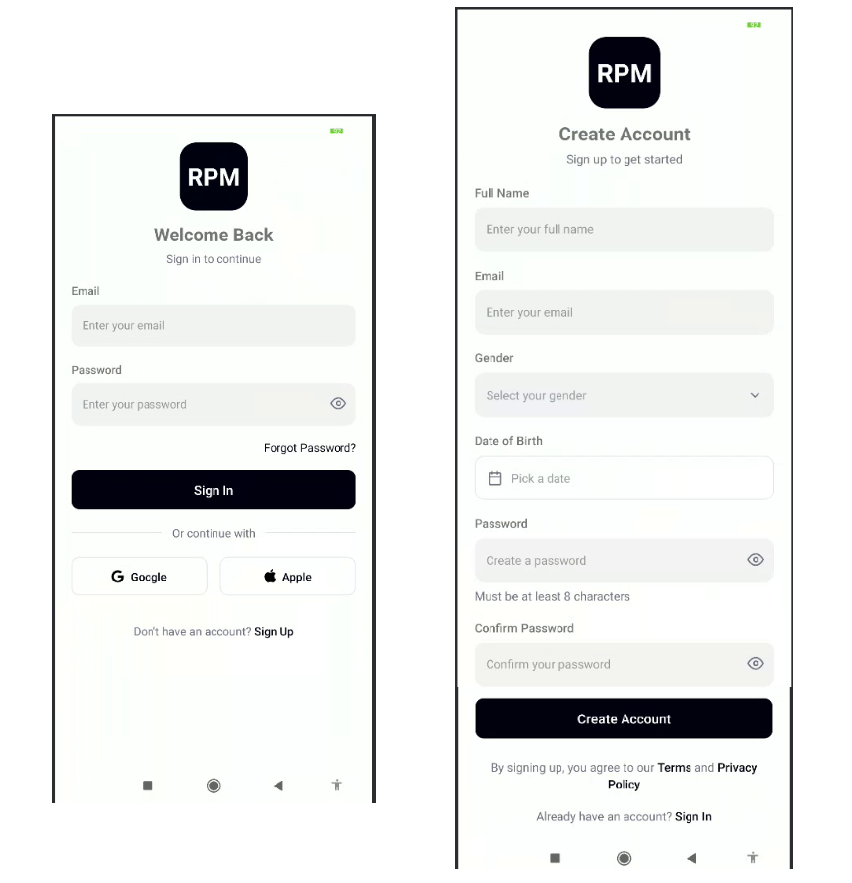
\includegraphics[width=\textwidth,keepaspectratio]{images/Chapter5/Mobile/mobile-auth-flow.png}
    \end{center}
    \caption{\textit{Màn hình đăng nhập, đăng ký và phân luồng người dùng trên ứng dụng di động}}
    \label{chapter5-image01}
    \end{figure}
\end{center}

\subsubsection{Trang chủ dành cho bệnh nhân}
\par Sau khi đăng nhập bằng tài khoản bệnh nhân, người dùng được chuyển đến trang chủ của ứng dụng. Trang chủ đóng vai trò là màn hình tổng quan, giúp bệnh nhân nhanh chóng nắm bắt tình trạng theo dõi hiện tại. Từ màn hình này, bệnh nhân có thể truy cập nhanh đến các chức năng quan trọng như nhập chỉ số mới, xem lịch sử đo, xem cảnh báo, mở thông báo và trao đổi với bác sĩ. Việc gom các thao tác chính vào trang chủ giúp bệnh nhân không cần phải tìm kiếm nhiều trong ứng dụng, đặc biệt phù hợp với nhóm người dùng lớn tuổi hoặc không quen thao tác trên các ứng dụng phức tạp.

\par Trang chủ cũng có thể hiển thị các thông tin tóm tắt như chỉ số gần nhất, trạng thái cảnh báo, số lượng thông báo chưa đọc hoặc lời nhắc cần thực hiện. Những thông tin này giúp bệnh nhân có cái nhìn nhanh về tình trạng sức khỏe của mình mà không cần mở từng màn hình riêng lẻ. Đây là một điểm quan trọng trong ứng dụng RPM vì người bệnh cần theo dõi đều đặn nhưng thao tác phải nhanh, dễ hiểu và không gây áp lực sử dụng.

\begin{center}
    \begin{figure}[H]
    \begin{center}
     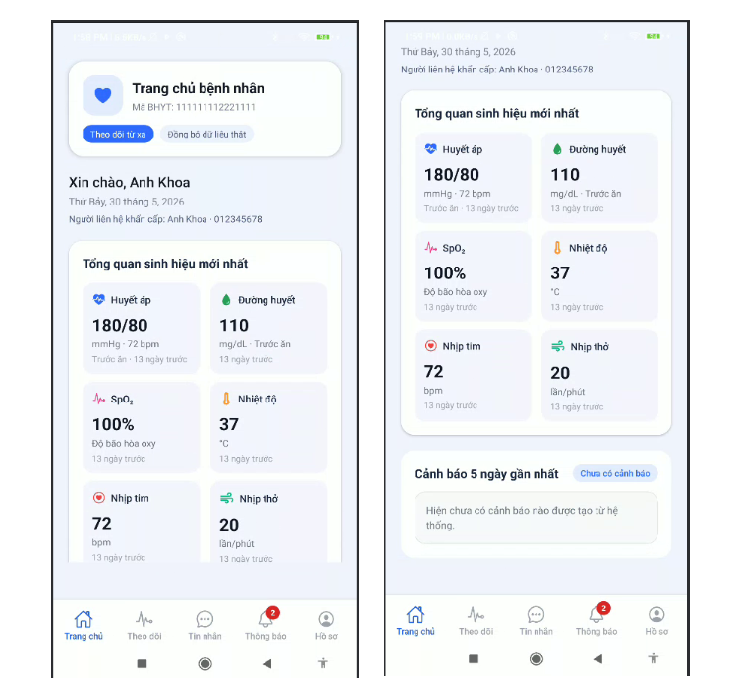
\includegraphics[width=\textwidth,keepaspectratio]{images/Chapter5/Mobile/mobile-patient-home.png}
    \end{center}
    \caption{\textit{Màn hình trang chủ dành cho bệnh nhân}}
    \label{chapter5-image02}
    \end{figure}
\end{center}

\subsubsection{Nhập chỉ số sức khỏe}
\par Chức năng nhập chỉ số sức khỏe là chức năng cốt lõi của ứng dụng di động. Bệnh nhân có thể nhập các dữ liệu liên quan đến quá trình theo dõi bệnh mãn tính như huyết áp tâm thu, huyết áp tâm trương, đường huyết, nhịp tim, thân nhiệt, SpO2 và nhịp thở. Các chỉ số này được gửi về backend để lưu trữ, đồng thời được sử dụng làm đầu vào cho cơ chế đánh giá ngưỡng và sinh cảnh báo tự động.

\par Giao diện nhập liệu được thiết kế theo hướng chia các nhóm chỉ số rõ ràng, có nhãn và đơn vị đo tương ứng để hạn chế sai sót. Với huyết áp, hệ thống ghi nhận huyết áp tâm thu và huyết áp tâm trương, sau đó backend có thể tính toán thêm chỉ số MAP để phục vụ theo dõi. Với đường huyết, hệ thống cho phép ghi nhận giá trị đường huyết kèm bối cảnh đo như trước ăn hoặc sau ăn nếu cần. Khi bệnh nhân nhấn lưu, ứng dụng gửi request đến API tạo bản đo, sau đó hiển thị kết quả thành công hoặc thông báo lỗi nếu dữ liệu không hợp lệ.

\begin{center}
    \begin{figure}[H]
    \begin{center}
     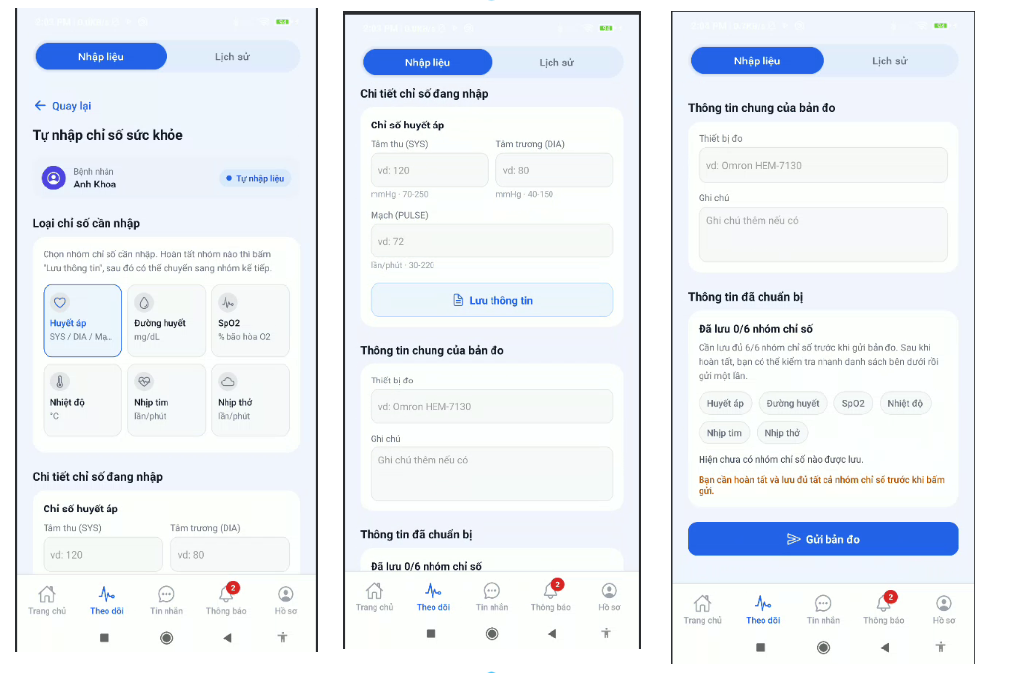
\includegraphics[width=\textwidth,keepaspectratio]{images/Chapter5/Mobile/mobile-input-measurement.png}
    \end{center}
    \caption{\textit{Màn hình nhập chỉ số sức khỏe của bệnh nhân}}
    \label{chapter5-image03}
    \end{figure}
\end{center}

\subsubsection{Theo dõi các chỉ số sức khỏe}
\par Bên cạnh việc nhập dữ liệu, bệnh nhân có thể sử dụng màn hình theo dõi để quan sát các chỉ số sức khỏe của mình theo thời gian. Màn hình này giúp người dùng không chỉ xem một lần đo đơn lẻ mà còn hiểu được xu hướng thay đổi của các chỉ số. Ví dụ, bệnh nhân có thể nhận thấy huyết áp có xu hướng tăng trong vài ngày gần đây, đường huyết thường cao sau bữa ăn hoặc SpO2 duy trì ổn định trong khoảng an toàn. Việc trực quan hóa dữ liệu giúp người bệnh có thêm động lực theo dõi và chủ động hơn trong việc chăm sóc sức khỏe cá nhân.

\par Dữ liệu theo dõi được lấy từ các lần đo đã lưu trong hệ thống. Ứng dụng có thể hiển thị thông tin dưới dạng thẻ chỉ số, biểu đồ hoặc danh sách tóm tắt tùy theo từng màn hình. Cách trình bày này phù hợp với mục tiêu của đề tài vì hệ thống không chỉ lưu dữ liệu, mà còn giúp người bệnh và nhân viên y tế dễ dàng quan sát diễn biến sức khỏe theo thời gian.

\begin{center}
    \begin{figure}[H]
    \begin{center}
     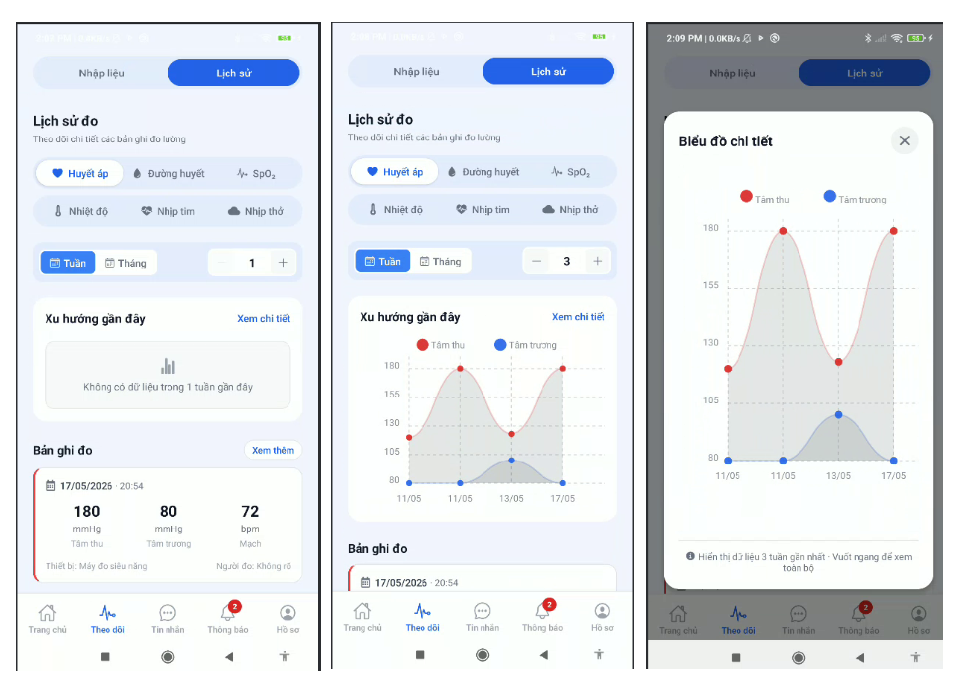
\includegraphics[width=\textwidth,keepaspectratio]{images/Chapter5/Mobile/mobile-tracking.png}
    \end{center}
    \caption{\textit{Màn hình theo dõi các chỉ số sức khỏe của bệnh nhân}}
    \label{chapter5-image04}
    \end{figure}
\end{center}

\subsubsection{Xem lịch sử đo}
\par Chức năng xem lịch sử đo cho phép bệnh nhân tra cứu lại các lần đo đã nhập trước đó. Mỗi bản ghi đo có thể bao gồm thời gian đo, loại chỉ số, giá trị huyết áp, đường huyết, nhịp tim, thân nhiệt, SpO2, nhịp thở và các ghi chú liên quan. Đây là chức năng thay thế cho việc ghi chép thủ công bằng sổ tay, giúp bệnh nhân giảm rủi ro thất lạc dữ liệu, ghi sai thời điểm hoặc không thể tổng hợp dữ liệu khi cần trao đổi với bác sĩ.

\par Màn hình lịch sử đo hỗ trợ phân loại dữ liệu theo từng nhóm chỉ số, giúp người dùng dễ tập trung vào loại dữ liệu mình quan tâm. Ví dụ, bệnh nhân có thể xem riêng lịch sử huyết áp, đường huyết, SpO2 hoặc thân nhiệt. Điều này đặc biệt hữu ích đối với bệnh nhân mắc đồng thời nhiều bệnh lý mãn tính, khi mỗi loại chỉ số có ý nghĩa khác nhau trong quá trình theo dõi. Các dữ liệu lịch sử cũng là nguồn đầu vào quan trọng để bác sĩ quan sát biểu đồ xu hướng trên ứng dụng web.

\begin{center}
    \begin{figure}[H]
    \begin{center}
     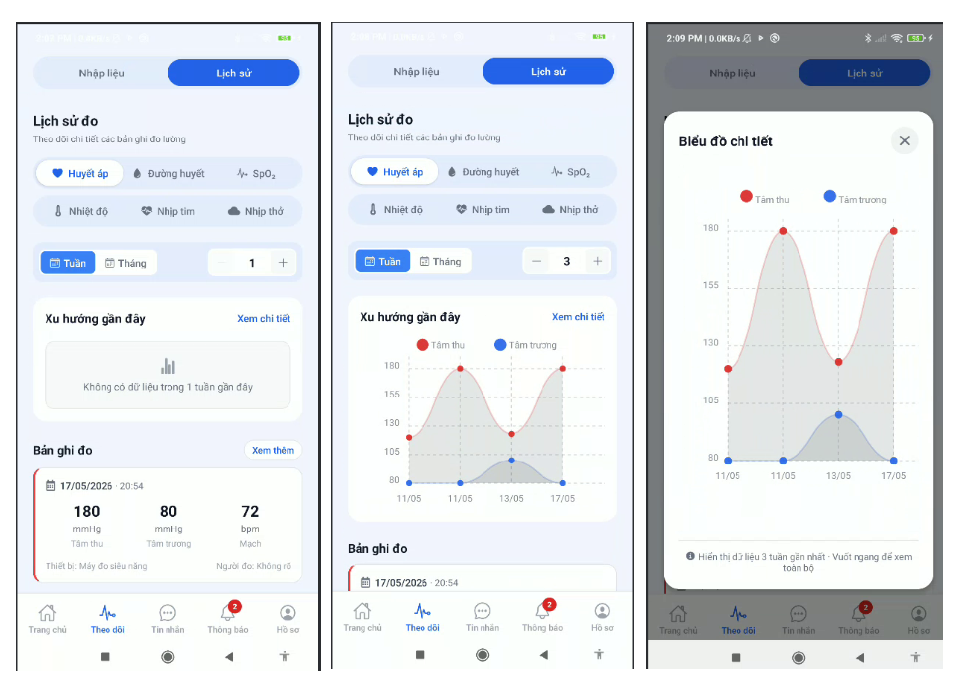
\includegraphics[width=\textwidth,keepaspectratio]{images/Chapter5/Mobile/mobile-history.png}
    \end{center}
    \caption{\textit{Màn hình lịch sử đo chỉ số sức khỏe}}
    \label{chapter5-image05}
    \end{figure}
\end{center}

\subsubsection{Xem cảnh báo chỉ số bất thường}
\par Khi hệ thống phát hiện một hoặc nhiều chỉ số vượt ngưỡng an toàn, cảnh báo sẽ được tạo và bệnh nhân có thể xem trong màn hình cảnh báo. Mỗi cảnh báo hiển thị thông tin về thời điểm phát sinh, loại chỉ số vi phạm, giá trị đã đo, ngưỡng tham chiếu và trạng thái xử lý. Nhờ đó, bệnh nhân có thể nhận biết rõ chỉ số nào đang bất thường thay vì chỉ nhận một thông báo chung chung.

\par Cảnh báo được nhóm theo ngày và có thể được phân biệt theo trạng thái hoặc mức độ nghiêm trọng. Khi chọn một cảnh báo, bệnh nhân có thể xem thông tin chi tiết hơn, bao gồm danh sách các vi phạm trong cùng một lần đo. Cách trình bày này giúp bệnh nhân hiểu được nguyên nhân cảnh báo, đồng thời hỗ trợ việc trao đổi với bác sĩ nếu cần tư vấn thêm. Đối với một hệ thống theo dõi từ xa, chức năng cảnh báo đóng vai trò rất quan trọng vì nó giúp chuyển hệ thống từ trạng thái lưu trữ dữ liệu thụ động sang hỗ trợ phát hiện bất thường chủ động.

\begin{center}
    \begin{figure}[H]
    \begin{center}
     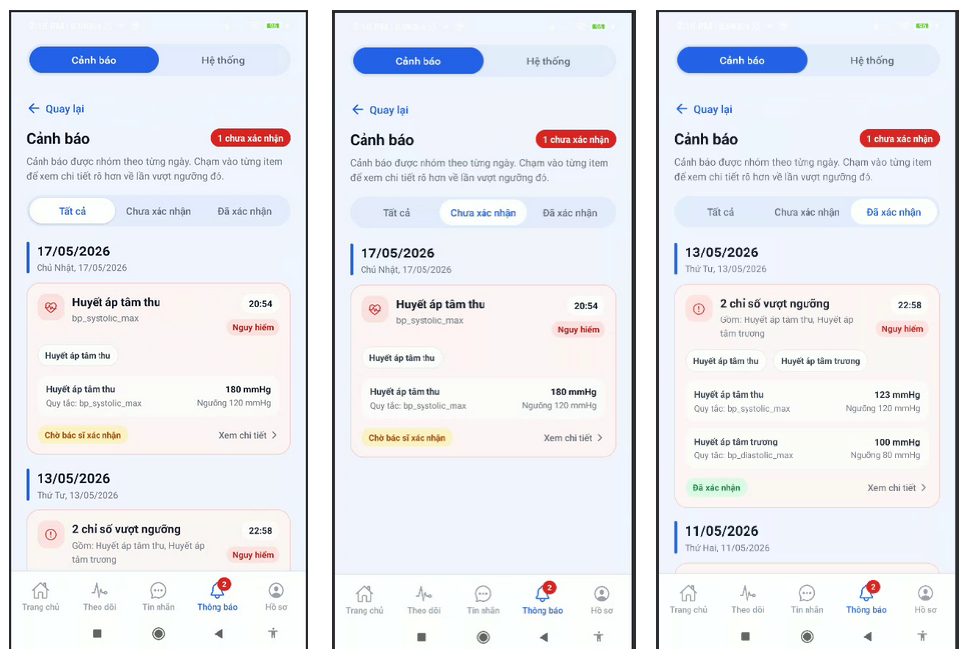
\includegraphics[width=\textwidth,keepaspectratio]{images/Chapter5/Mobile/mobile-alerts.png}
    \end{center}
    \caption{\textit{Màn hình danh sách và chi tiết cảnh báo của bệnh nhân}}
    \label{chapter5-image06}
    \end{figure}
\end{center}

\subsubsection{Trung tâm thông báo}
\par Ứng dụng di động cung cấp màn hình thông báo để bệnh nhân xem lại các thông báo đã nhận. Thông báo có thể liên quan đến cảnh báo chỉ số bất thường, nhắc nhở đo chỉ số, nhắc nhở dùng thuốc hoặc các sự kiện khác trong quá trình theo dõi. Việc lưu thông báo trong ứng dụng giúp người dùng có thể xem lại nội dung sau khi thông báo đẩy đã biến mất khỏi thanh thông báo của thiết bị.

\par Mỗi thông báo có thể có trạng thái đã đọc hoặc chưa đọc, đồng thời có dữ liệu điều hướng để đưa người dùng đến màn hình liên quan. Ví dụ, nếu thông báo liên quan đến cảnh báo, bệnh nhân có thể nhấn vào thông báo để mở màn hình cảnh báo tương ứng. Nếu thông báo liên quan đến nhắc nhở, bệnh nhân có thể mở ứng dụng để thực hiện việc đo chỉ số hoặc xem nội dung nhắc nhở. Chức năng này giúp tăng tính liên tục trong quá trình theo dõi sức khỏe từ xa.

\begin{center}
    \begin{figure}[H]
    \begin{center}
     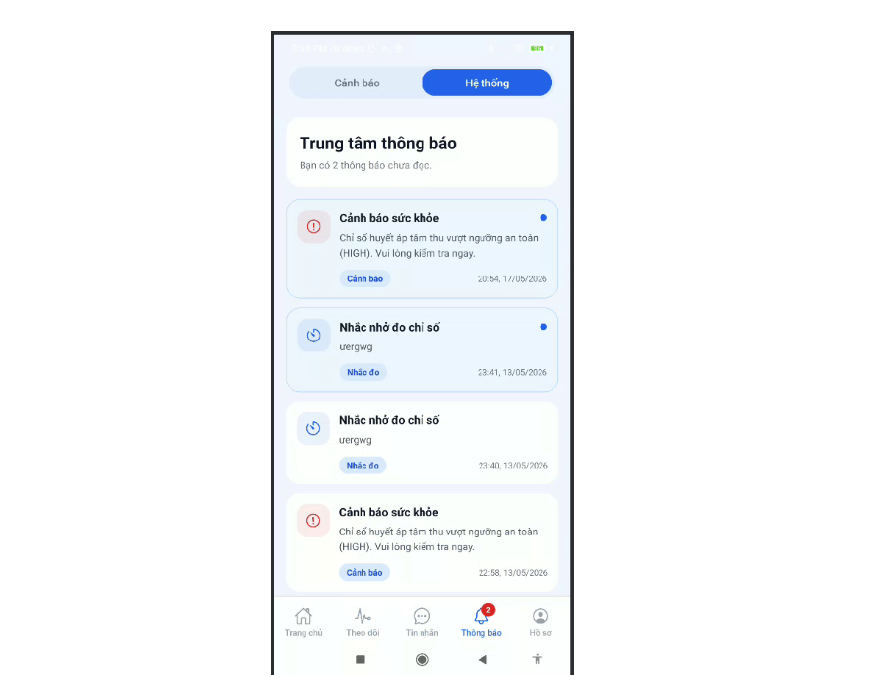
\includegraphics[width=\textwidth,keepaspectratio]{images/Chapter5/Mobile/mobile-notifications.png}
    \end{center}
    \caption{\textit{Màn hình trung tâm thông báo trên ứng dụng di động}}
    \label{chapter5-image07}
    \end{figure}
\end{center}

\subsubsection{Nhắn tin với bác sĩ}
\par Ứng dụng di động hỗ trợ bệnh nhân trao đổi tin nhắn với bác sĩ phụ trách. Chức năng này giúp bệnh nhân có thể gửi câu hỏi, phản hồi tình trạng sức khỏe hoặc trao đổi thêm khi xuất hiện cảnh báo bất thường. Tin nhắn được đồng bộ với hệ thống backend và hiển thị ở cả phía bệnh nhân lẫn phía bác sĩ, tạo ra một kênh liên lạc trực tiếp bên trong hệ thống thay vì phụ thuộc hoàn toàn vào điện thoại hoặc các ứng dụng nhắn tin bên ngoài.

\par Đặc biệt, một số tin nhắn có thể được tạo tự động từ hệ thống khi phát sinh cảnh báo. Tin nhắn hệ thống có thể chứa thông tin tóm tắt về chỉ số vượt ngưỡng, giúp bác sĩ khi mở cuộc trò chuyện có thể nhanh chóng hiểu ngữ cảnh đang được trao đổi. Bệnh nhân cũng có thể xem lại các nội dung tư vấn trước đó trong cùng một màn hình chat, từ đó quá trình theo dõi và phản hồi trở nên liền mạch hơn.

\begin{center}
    \begin{figure}[H]
    \begin{center}
     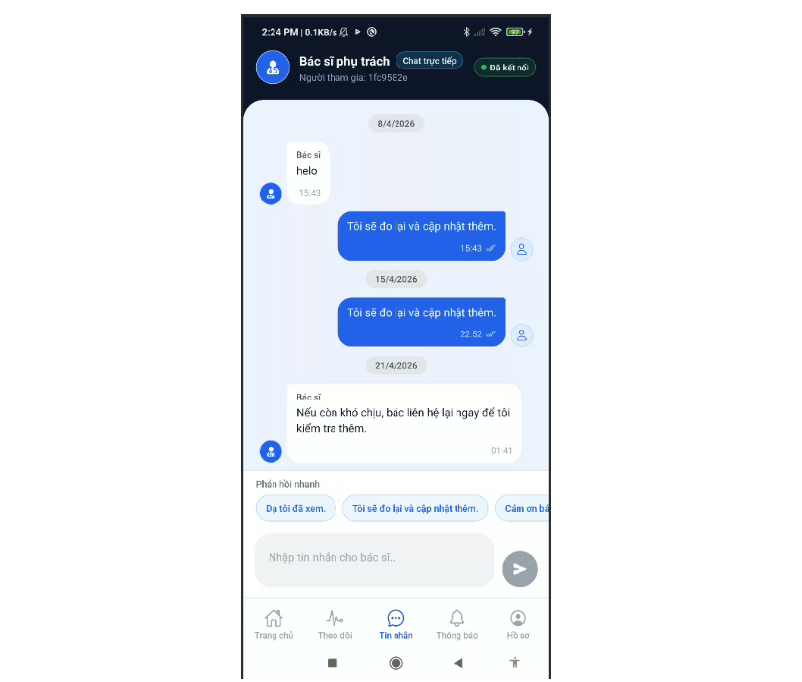
\includegraphics[width=\textwidth,keepaspectratio]{images/Chapter5/Mobile/mobile-doctor-chat.png}
    \end{center}
    \caption{\textit{Màn hình trao đổi tin nhắn giữa bệnh nhân và bác sĩ}}
    \label{chapter5-image08}
    \end{figure}
\end{center}

\subsubsection{Quản lý hồ sơ cá nhân}
\par Bệnh nhân có thể xem và cập nhật một số thông tin hồ sơ cá nhân trên ứng dụng di động. Hồ sơ có thể bao gồm họ tên, email, số điện thoại, ngày sinh, giới tính, ảnh đại diện, thông tin bảo hiểm, CCCD, địa chỉ, liên hệ khẩn cấp và tiền sử bệnh. Những thông tin này giúp bác sĩ và nhân viên y tế có thêm ngữ cảnh khi theo dõi dữ liệu đo của bệnh nhân.

\par Việc cho phép bệnh nhân tự cập nhật thông tin cá nhân giúp giảm khối lượng công việc cho quản trị viên và hạn chế dữ liệu hồ sơ bị lỗi thời. Đồng thời, ứng dụng cũng hỗ trợ chức năng đăng xuất để người dùng kết thúc phiên làm việc khi cần thiết. Đây là những chức năng tuy không trực tiếp liên quan đến cảnh báo chỉ số, nhưng cần thiết để tạo nên một ứng dụng hoàn chỉnh và có thể sử dụng trong thực tế.

\begin{center}
    \begin{figure}[H]
    \begin{center}
     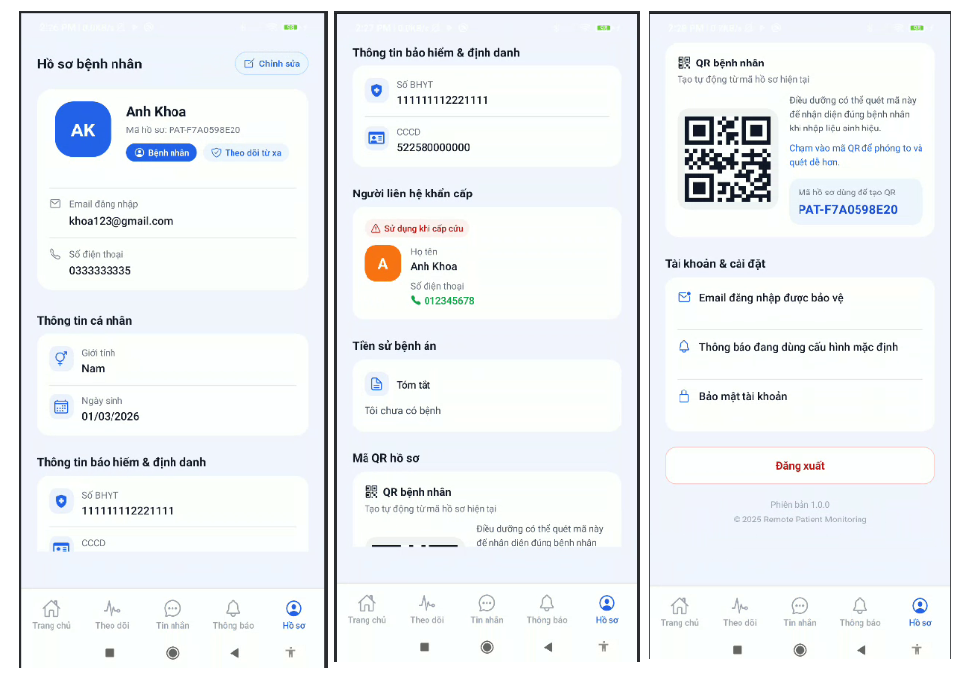
\includegraphics[width=\textwidth,keepaspectratio]{images/Chapter5/Mobile/mobile-patient-profile.png}
    \end{center}
    \caption{\textit{Màn hình hồ sơ cá nhân của bệnh nhân}}
    \label{chapter5-image09}
    \end{figure}
\end{center}

\subsubsection{Danh sách bệnh nhân dành cho y tá}
\par Với tài khoản y tá, ứng dụng hiển thị màn hình danh sách các bệnh nhân được phân công theo dõi. Màn hình này cho phép y tá xem tổng số bệnh nhân, số bệnh nhân đang có cảnh báo, tìm kiếm bệnh nhân theo tên hoặc mã hồ sơ và lọc các bệnh nhân cần chú ý. Đây là chức năng quan trọng trong trường hợp cơ sở y tế muốn y tá hỗ trợ bác sĩ theo dõi bệnh nhân hằng ngày.

\par Mỗi bệnh nhân trong danh sách được hiển thị dưới dạng thẻ thông tin, bao gồm các dữ liệu nhận diện cơ bản và trạng thái cảnh báo nếu có. Y tá có thể chọn một bệnh nhân để xem chi tiết hoặc chuyển sang luồng nhập liệu. Việc giới hạn danh sách theo phân công giúp y tá chỉ nhìn thấy những bệnh nhân thuộc phạm vi phụ trách, phù hợp với yêu cầu kiểm soát truy cập dữ liệu trong hệ thống y tế.

\begin{center}
    \begin{figure}[H]
    \begin{center}
     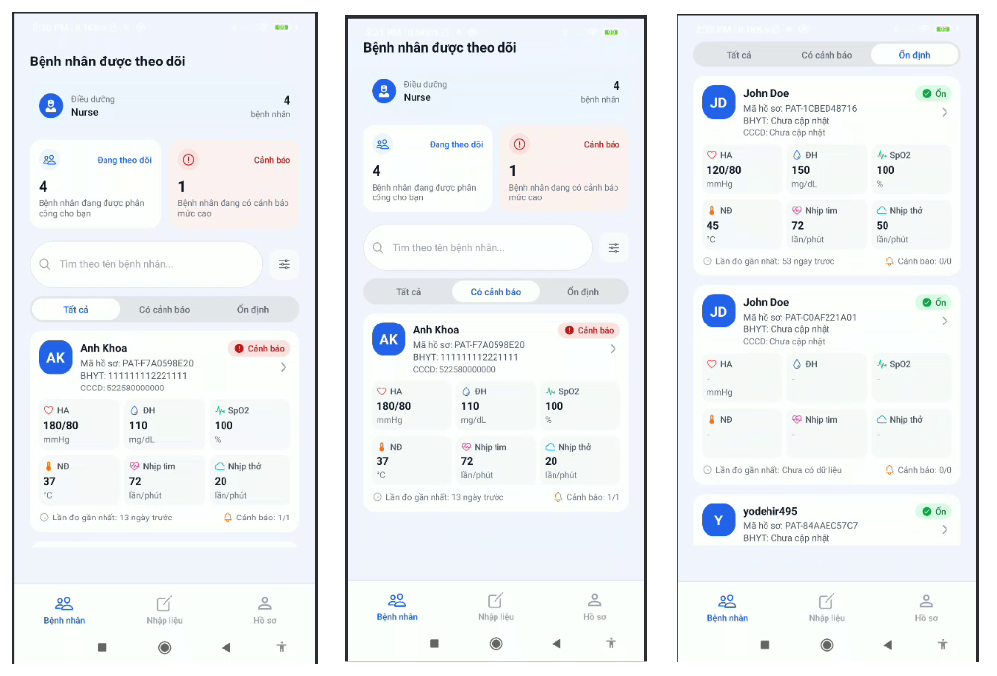
\includegraphics[width=\textwidth,keepaspectratio]{images/Chapter5/Mobile/mobile-nurse-patient-list.png}
    \end{center}
    \caption{\textit{Màn hình danh sách bệnh nhân được phân công cho y tá}}
    \label{chapter5-image10}
    \end{figure}
\end{center}

\subsubsection{Y tá nhập chỉ số cho bệnh nhân}
\par Ngoài bệnh nhân tự nhập dữ liệu, hệ thống còn hỗ trợ y tá nhập chỉ số cho bệnh nhân. Chức năng này phù hợp với trường hợp bệnh nhân đang được đo tại cơ sở y tế, bệnh nhân lớn tuổi, bệnh nhân không sử dụng điện thoại thông minh hoặc cần nhân viên y tế hỗ trợ ghi nhận dữ liệu. Y tá có thể chọn bệnh nhân từ danh sách được phân công, nhập mã hồ sơ hoặc quét mã QR để tải thông tin bệnh nhân trước khi nhập liệu.

\par Sau khi bệnh nhân được chọn, y tá nhập các chỉ số sức khỏe tương tự như luồng bệnh nhân tự nhập. Dữ liệu sau đó được gửi lên backend và vẫn đi qua cùng một cơ chế lưu trữ, đánh giá ngưỡng, sinh cảnh báo và thông báo. Việc dùng chung luồng xử lý phía backend giúp dữ liệu đo có tính nhất quán, dù được nhập bởi bệnh nhân hay bởi y tá.

\begin{center}
    \begin{figure}[H]
    \begin{center}
     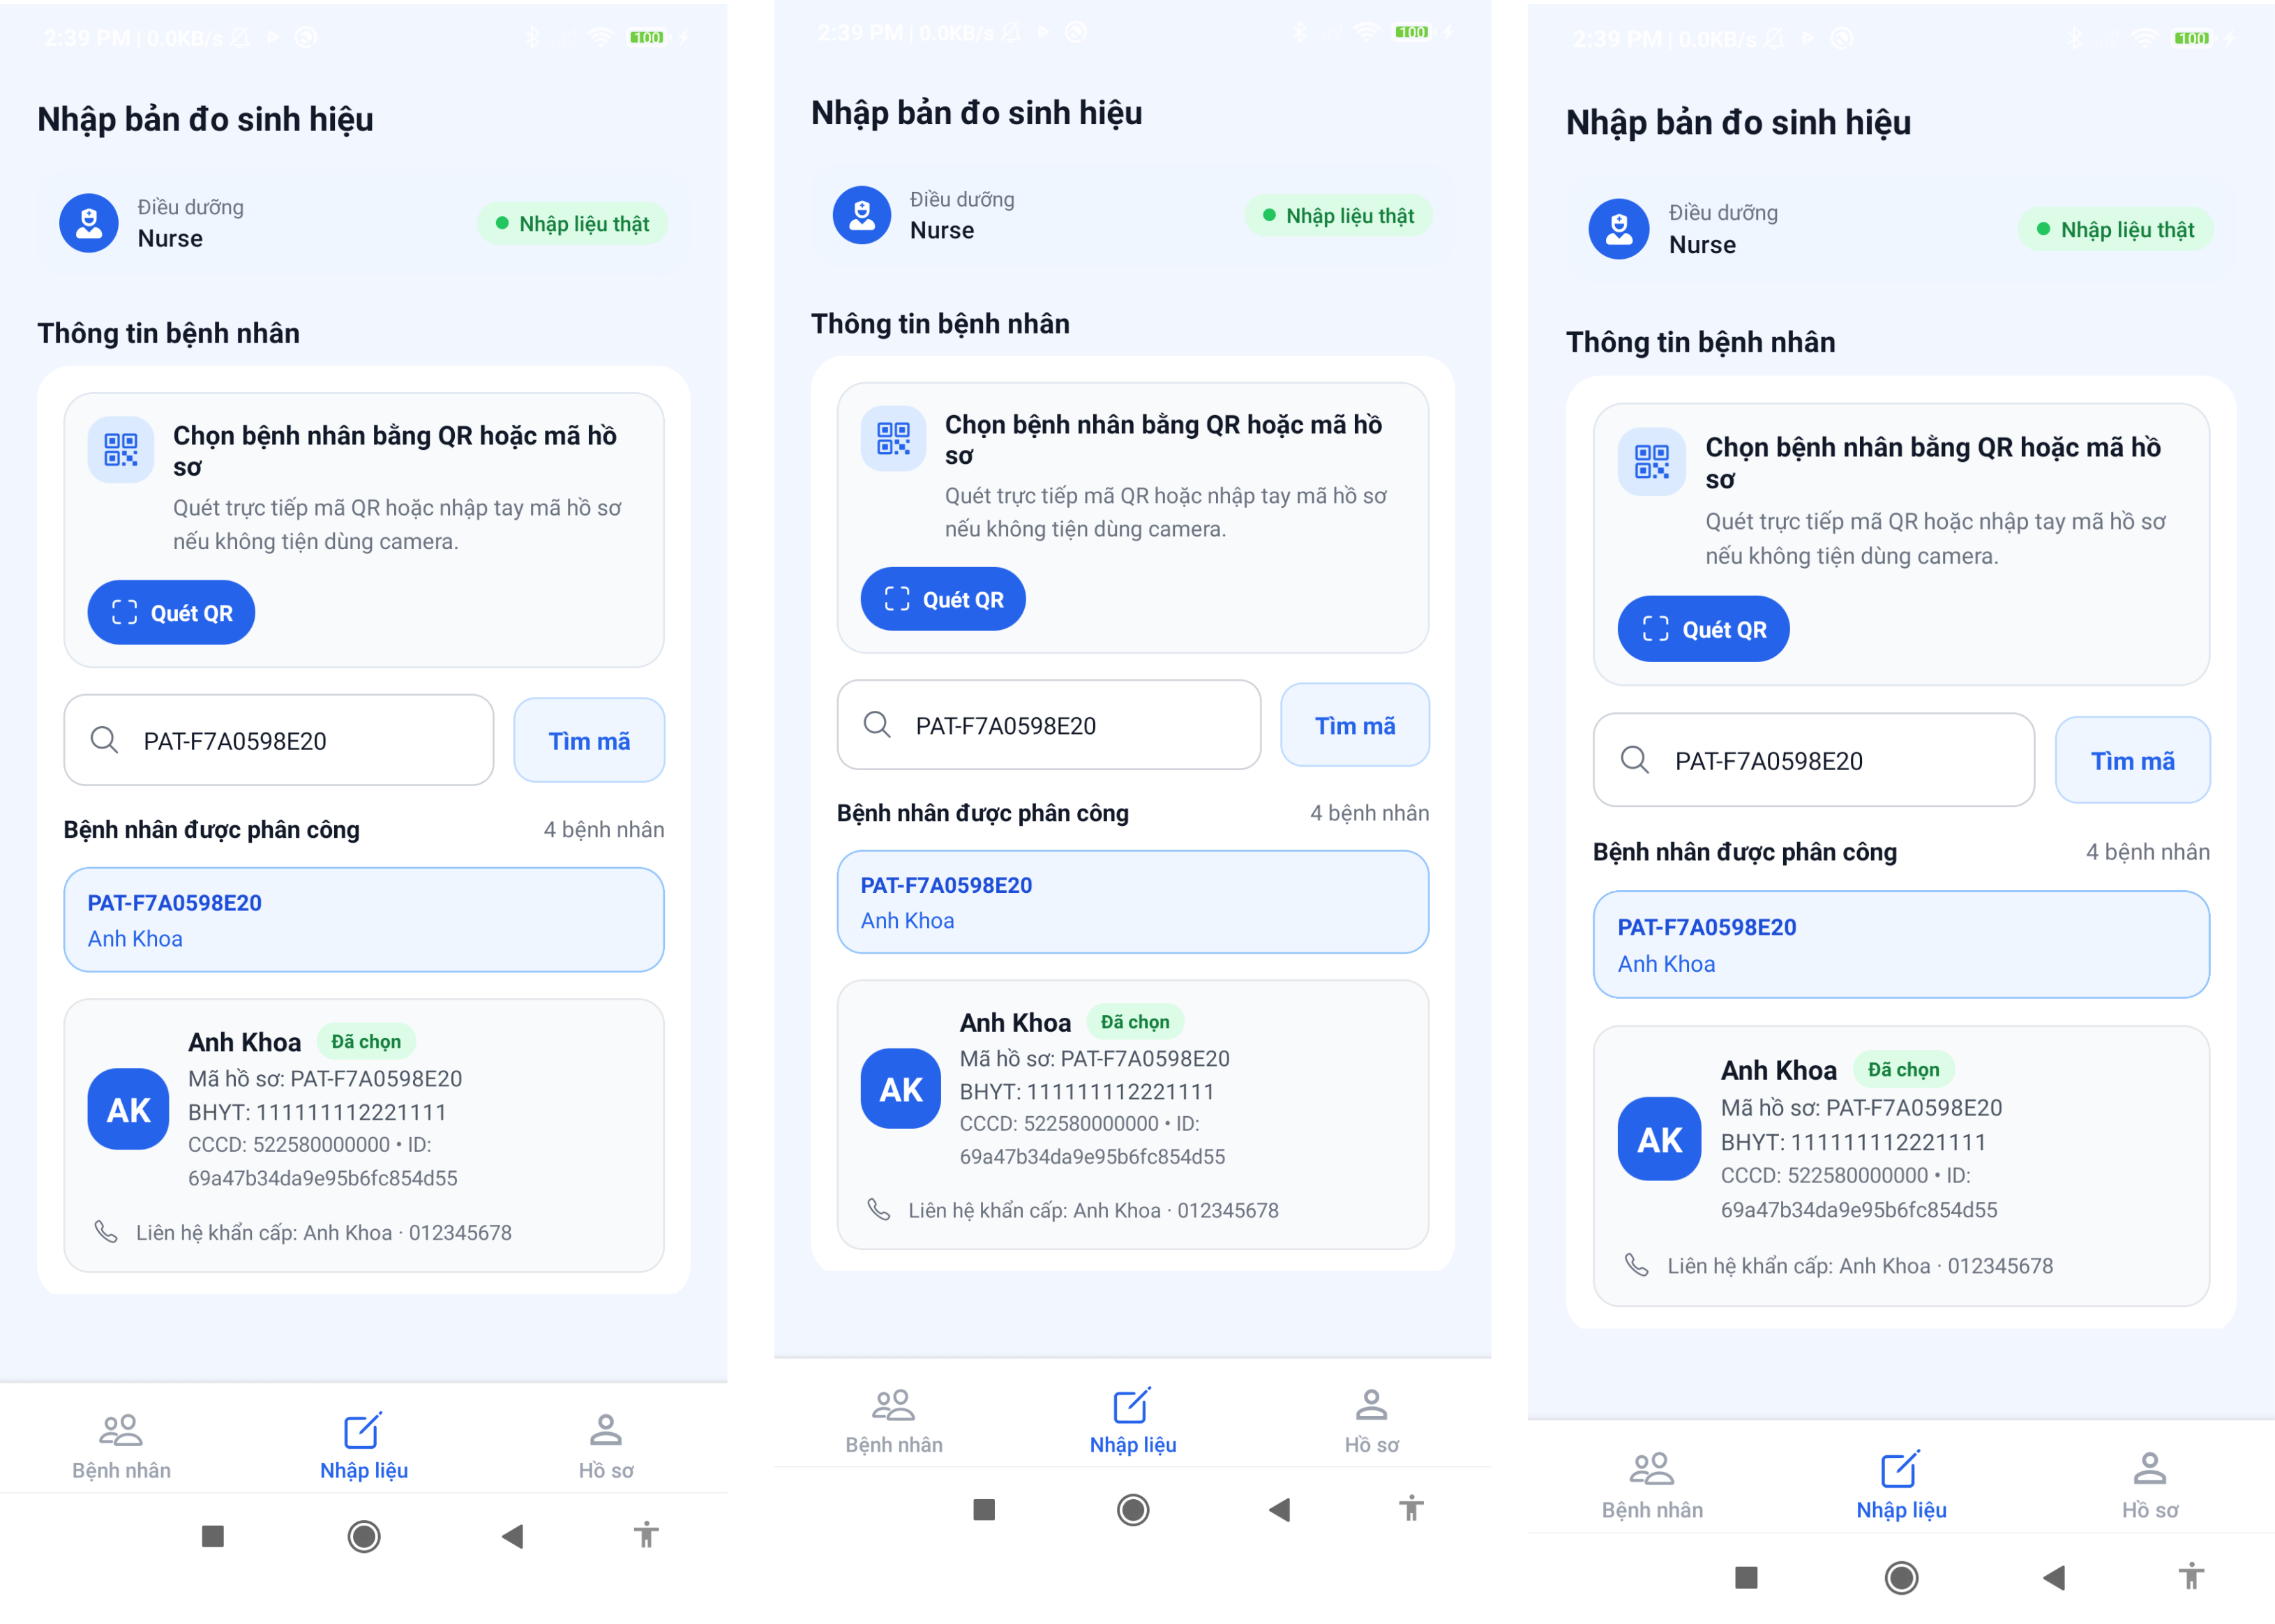
\includegraphics[width=\textwidth,keepaspectratio]{images/Chapter5/Mobile/mobile-nurse-input-measurement.png}
    \end{center}
    \caption{\textit{Màn hình y tá nhập chỉ số sức khỏe cho bệnh nhân}}
    \label{chapter5-image11}
    \end{figure}
\end{center}

\subsubsection{Hồ sơ y tá}
\par Ứng dụng di động cũng cung cấp màn hình hồ sơ dành cho y tá. Màn hình này hiển thị các thông tin như họ tên, email đăng nhập, số điện thoại, vai trò, khoa phòng, nơi làm việc, số chứng chỉ hành nghề, số năm kinh nghiệm, thời gian tạo hồ sơ và thời gian cập nhật gần nhất. Việc hiển thị thông tin chuyên môn giúp y tá kiểm tra lại hồ sơ của mình và tạo sự nhất quán với dữ liệu đang được quản trị viên quản lý trên trang admin.

\par Bên cạnh việc xem thông tin, y tá cũng có thể đăng xuất khỏi ứng dụng thông qua màn hình hồ sơ. Chức năng này giúp kết thúc phiên đăng nhập trên thiết bị, hạn chế rủi ro người khác truy cập vào dữ liệu bệnh nhân nếu thiết bị được dùng chung hoặc bị thất lạc.

\begin{center}
    \begin{figure}[H]
    \begin{center}
     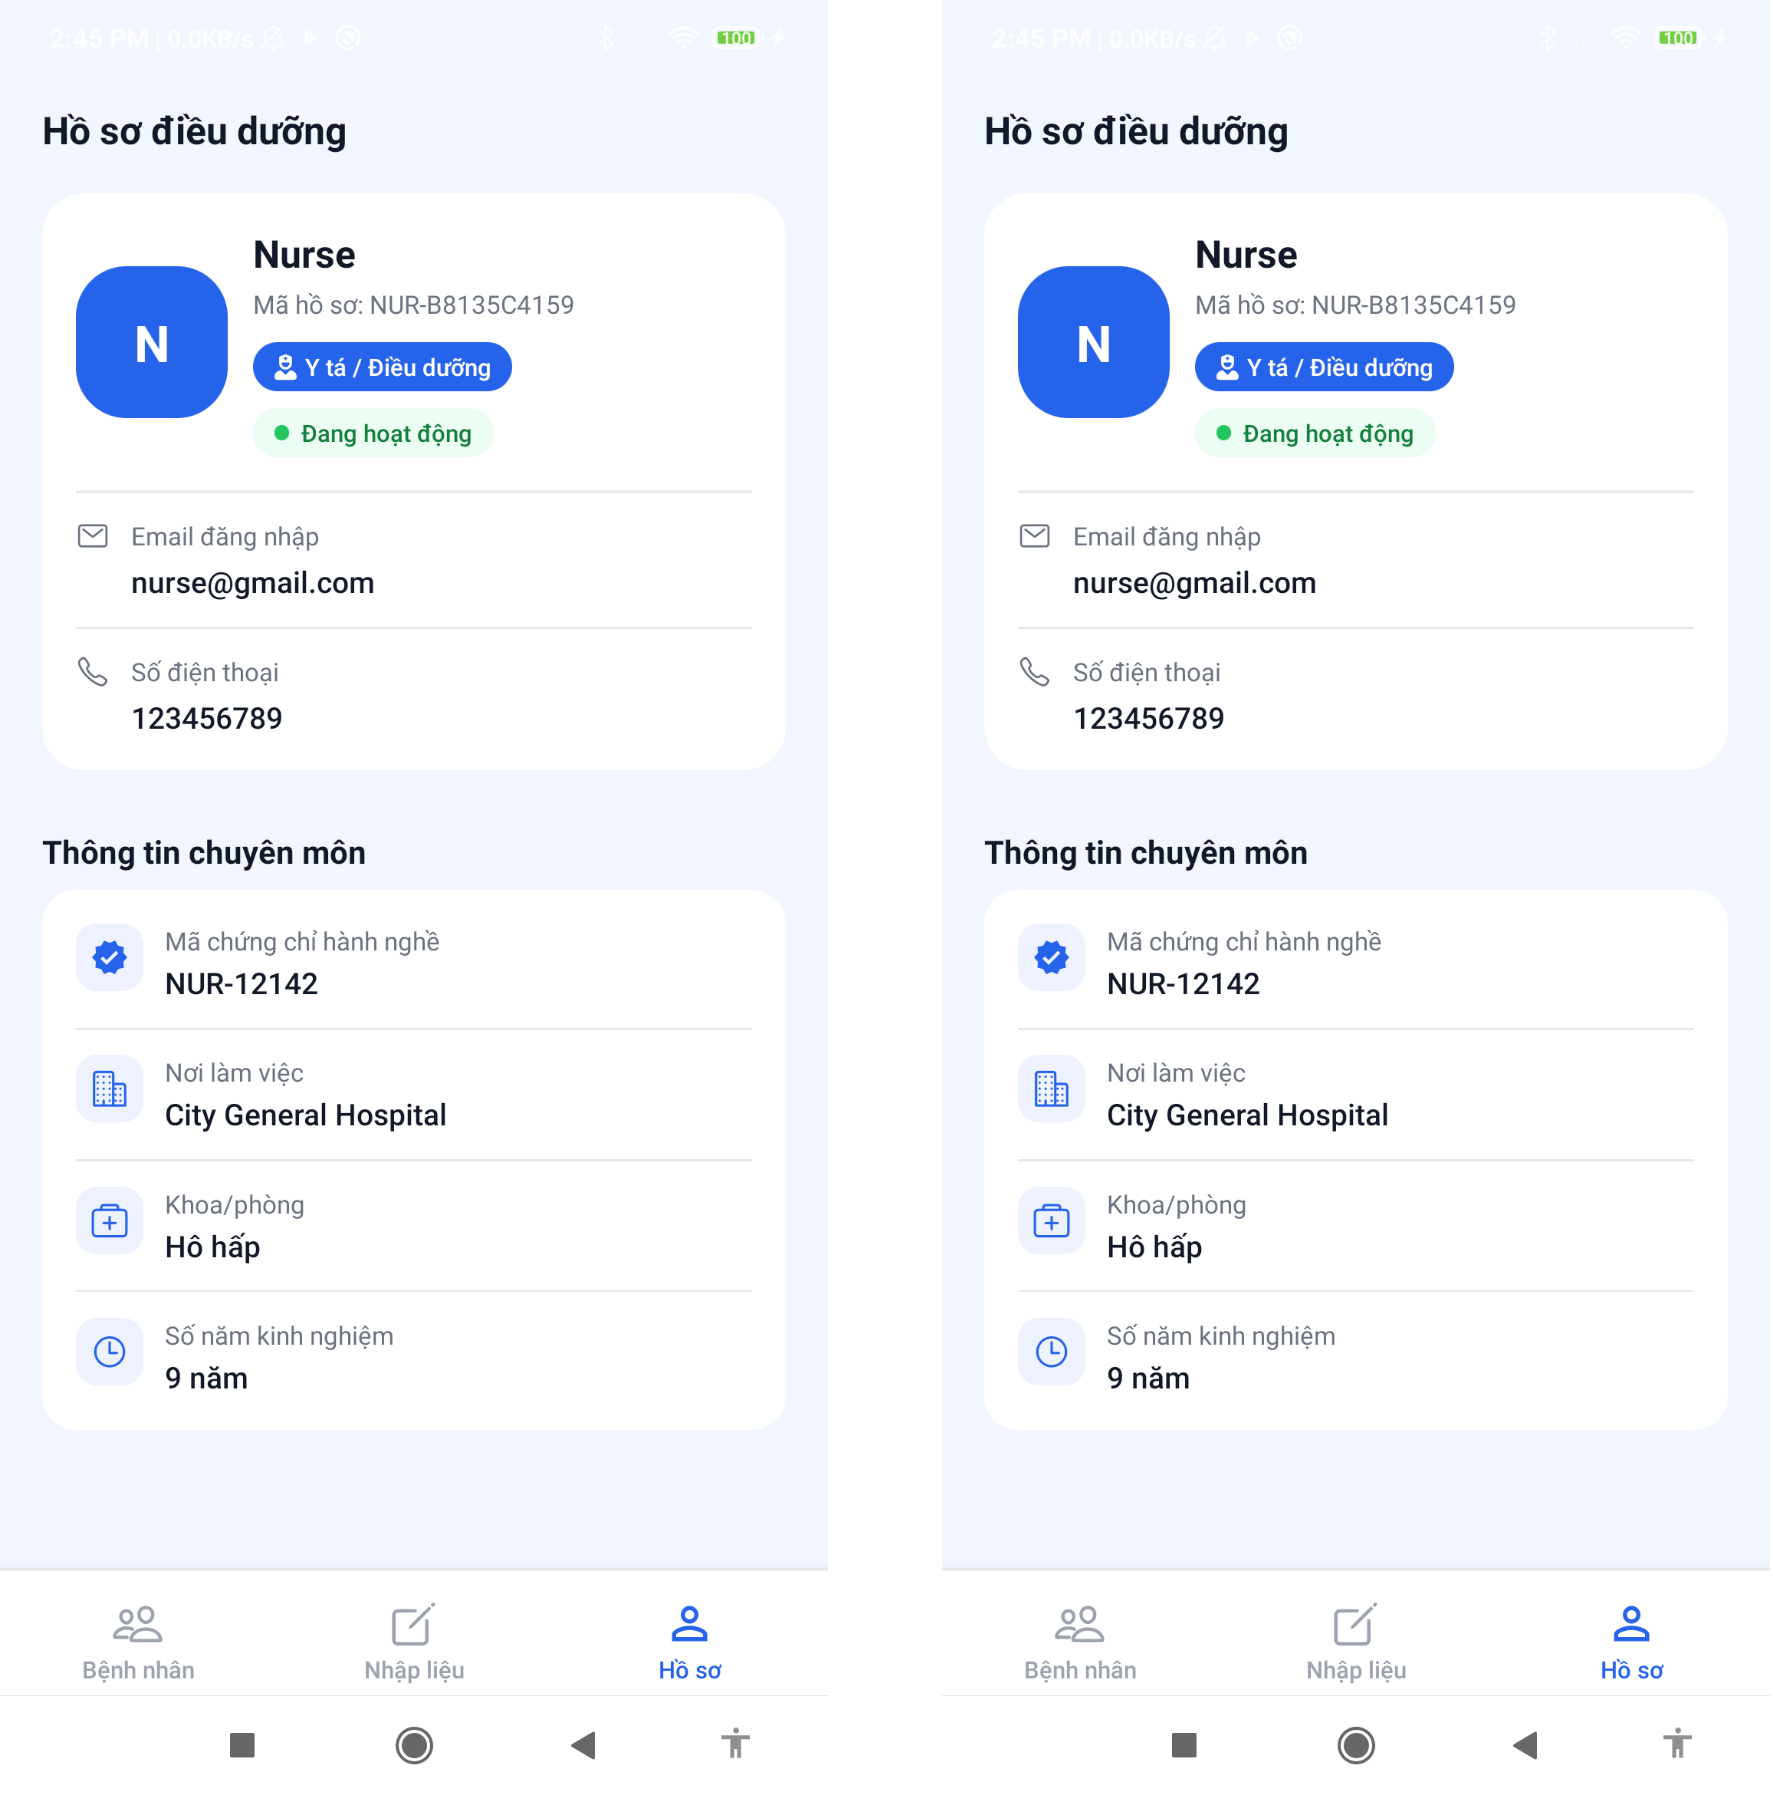
\includegraphics[width=\textwidth,keepaspectratio]{images/Chapter5/Mobile/mobile-nurse-profile.png}
    \end{center}
    \caption{\textit{Màn hình hồ sơ điều dưỡng trên ứng dụng di động}}
    \label{chapter5-image12}
    \end{figure}
\end{center}

\newpage
\subsection{Trang web dành cho bác sĩ}

\par Trang web dành cho bác sĩ là thành phần giúp bác sĩ theo dõi dữ liệu sức khỏe của các bệnh nhân được phân công. Ứng dụng web được thiết kế theo dạng dashboard quản lý, trong đó bác sĩ có thể xem tổng quan tình trạng bệnh nhân, truy cập danh sách bệnh nhân, xem chi tiết hồ sơ và lịch sử đo, cấu hình ngưỡng an toàn, theo dõi cảnh báo, tạo nhắc nhở và trao đổi tin nhắn với bệnh nhân. So với ứng dụng di động, trang web tận dụng lợi thế màn hình lớn để hiển thị nhiều dữ liệu hơn, đặc biệt là bảng dữ liệu, biểu đồ và các bộ lọc.

\subsubsection{Dashboard tổng quan}
\par Dashboard là màn hình đầu tiên sau khi bác sĩ đăng nhập vào hệ thống. Màn hình này hiển thị các thông tin tổng quan như tổng số bệnh nhân đang được theo dõi, số bệnh nhân ổn định, số bệnh nhân cần chú ý và danh sách cảnh báo gần đây. Các số liệu này giúp bác sĩ nhanh chóng nắm bắt tình hình chung mà không cần vào từng hồ sơ bệnh nhân riêng lẻ.

\par Dashboard cũng hỗ trợ biểu đồ tổng quan bệnh nhân theo khoảng thời gian. Bác sĩ có thể lọc cảnh báo theo ngày bắt đầu, ngày kết thúc và mức độ cảnh báo. Ngoài ra, hệ thống có chức năng xuất dữ liệu cảnh báo hoặc xuất báo cáo chỉ số sức khỏe ra file Excel. Đây là kết quả quan trọng vì báo cáo dạng file có thể được dùng để lưu trữ, trao đổi nội bộ hoặc phục vụ quá trình đánh giá sau này.

\begin{center}
    \begin{figure}[H]
    \begin{center}
     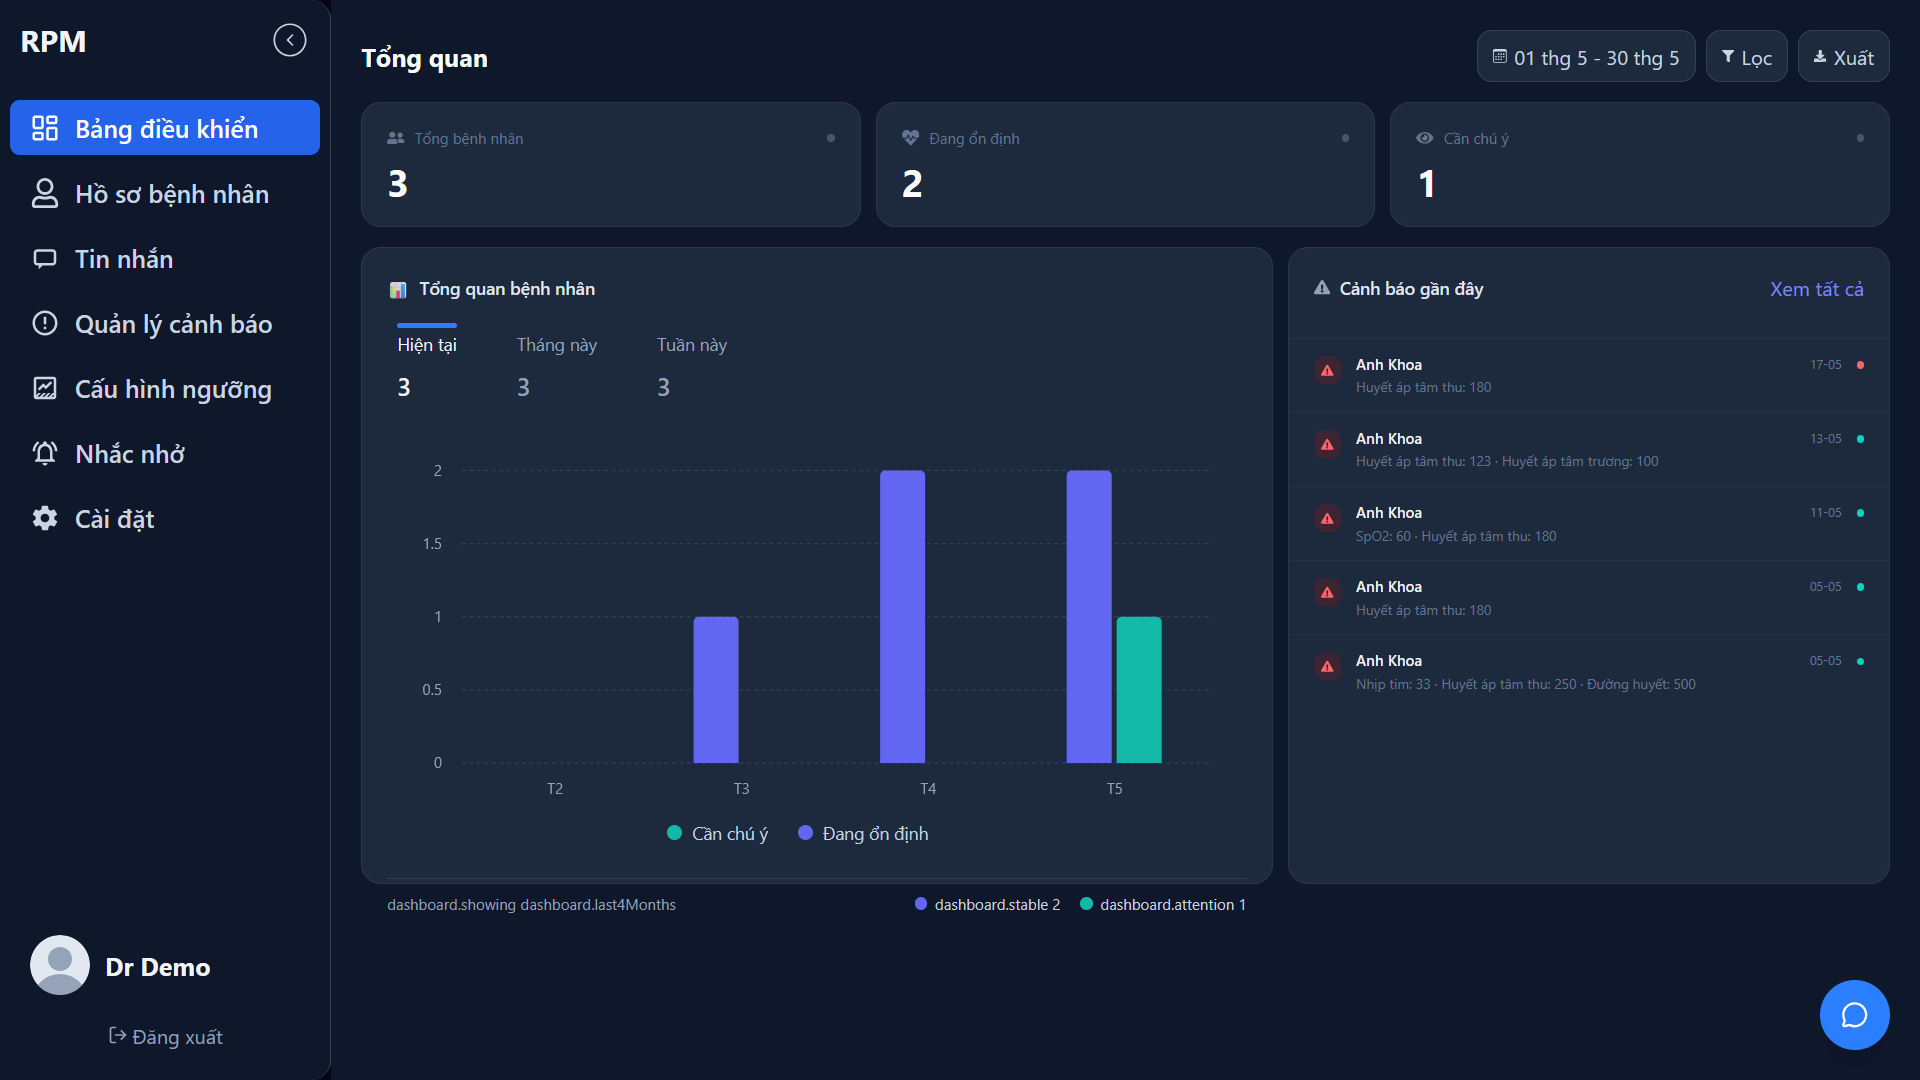
\includegraphics[width=\textwidth,keepaspectratio]{images/Chapter5/Web/web-doctor-dashboard.png}
    \end{center}
    \caption{\textit{Màn hình dashboard tổng quan dành cho bác sĩ}}
    \label{chapter5-image13}
    \end{figure}
\end{center}

\subsubsection{Xem danh sách bệnh nhân}
\par Màn hình danh sách bệnh nhân cho phép bác sĩ xem các bệnh nhân được phân công theo dõi. Mỗi bệnh nhân trong danh sách hiển thị các thông tin cơ bản như mã hồ sơ, họ tên, trạng thái theo dõi, thời điểm cập nhật và trạng thái cảnh báo nếu có. Bác sĩ có thể tìm kiếm hoặc lọc bệnh nhân để nhanh chóng xác định trường hợp cần quan tâm.

\par Chức năng này đóng vai trò như cửa ngõ để bác sĩ truy cập các thông tin chi tiết hơn. Từ danh sách bệnh nhân, bác sĩ có thể chọn một bệnh nhân để mở hồ sơ chi tiết, xem lịch sử đo, biểu đồ, ngưỡng an toàn, cảnh báo và nhắc nhở. Việc giới hạn danh sách theo phân công giúp hệ thống phù hợp hơn với quy trình vận hành thực tế, trong đó mỗi bác sĩ chỉ phụ trách một nhóm bệnh nhân nhất định.

\begin{center}
    \begin{figure}[H]
    \begin{center}
     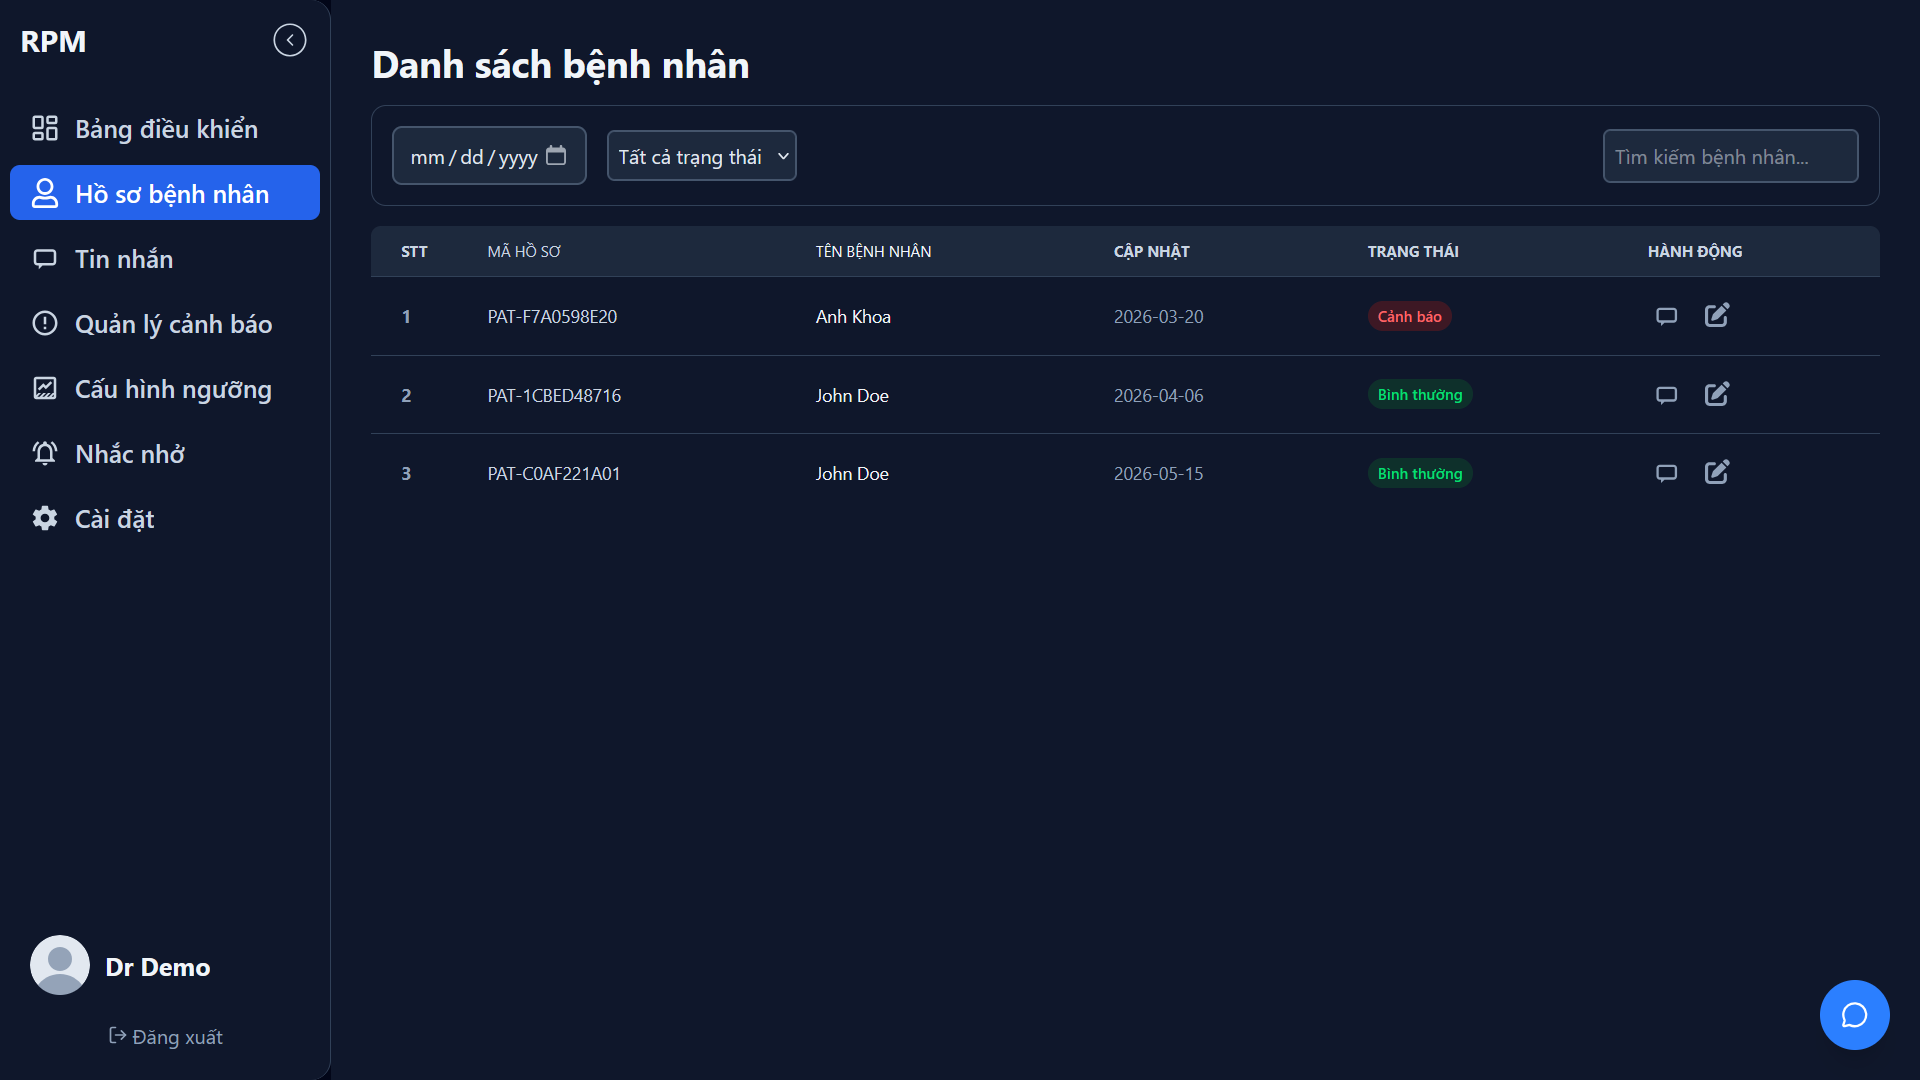
\includegraphics[width=\textwidth,keepaspectratio]{images/Chapter5/Web/web-patient-list.png}
    \end{center}
    \caption{\textit{Màn hình danh sách bệnh nhân được phân công cho bác sĩ}}
    \label{chapter5-image14}
    \end{figure}
\end{center}

\subsubsection{Xem thông tin chi tiết bệnh nhân}
\par Khi chọn một bệnh nhân, bác sĩ được chuyển đến màn hình chi tiết bệnh nhân. Màn hình này hiển thị thông tin cá nhân, mã hồ sơ, thông tin liên hệ, thông tin liên hệ khẩn cấp và các thông tin y tế cơ bản. Bên cạnh đó, hệ thống cũng hiển thị các ngưỡng chỉ số an toàn đã được thiết lập cho bệnh nhân nếu có. Nếu bệnh nhân chưa được cấu hình ngưỡng, bác sĩ có thể chuyển nhanh sang màn hình thiết lập ngưỡng để bổ sung.

\par Mục tiêu của màn hình chi tiết là cung cấp cho bác sĩ một cái nhìn đầy đủ về bệnh nhân trước khi đọc dữ liệu đo. Đối với bệnh nhân tăng huyết áp và đái tháo đường, cùng một giá trị đo có thể mang ý nghĩa khác nhau tùy vào tiền sử bệnh, độ tuổi, chỉ định theo dõi và tình trạng hiện tại. Vì vậy, việc đặt dữ liệu đo trong ngữ cảnh hồ sơ bệnh nhân giúp bác sĩ đánh giá thông tin một cách thuận tiện hơn.

\begin{center}
    \begin{figure}[H]
    \begin{center}
     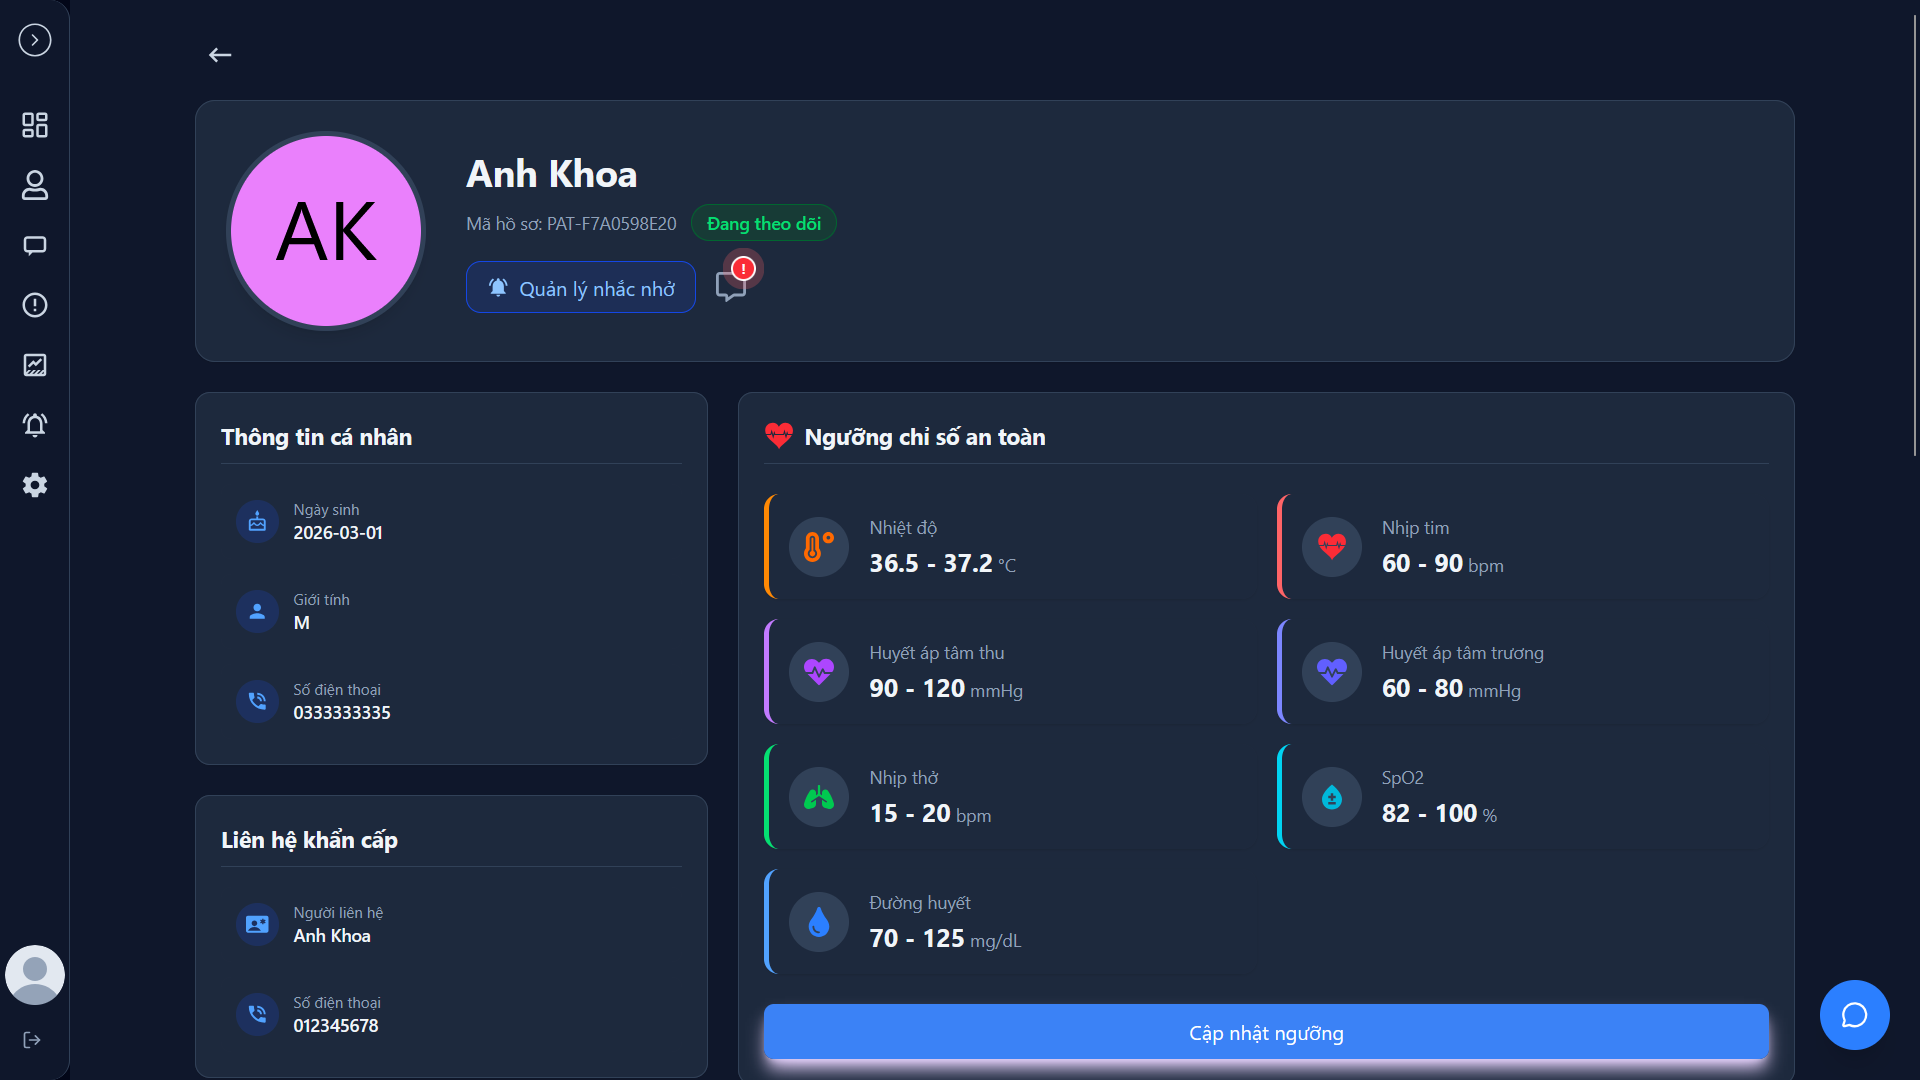
\includegraphics[width=\textwidth,keepaspectratio]{images/Chapter5/Web/web-patient-detail-info.png}
    \end{center}
    \caption{\textit{Màn hình thông tin chi tiết bệnh nhân}}
    \label{chapter5-image15}
    \end{figure}
\end{center}

\subsubsection{Xem biểu đồ xu hướng và lịch sử đo}
\par Trang chi tiết bệnh nhân cung cấp biểu đồ sức khỏe để bác sĩ theo dõi xu hướng thay đổi của các chỉ số theo thời gian. Các nhóm dữ liệu chính bao gồm huyết áp, đường huyết, thân nhiệt, SpO2, nhịp tim và nhịp thở. Bác sĩ có thể chuyển đổi giữa các khoảng thời gian như tuần gần nhất, nhiều tuần gần nhất hoặc nhiều tháng gần nhất để quan sát xu hướng ngắn hạn và dài hạn.

\par Bên cạnh biểu đồ, hệ thống cũng hiển thị bảng lịch sử đo gần đây. Bảng này cho phép bác sĩ xem từng bản ghi đo với thời điểm và giá trị cụ thể. Sự kết hợp giữa biểu đồ và bảng dữ liệu giúp bác sĩ vừa có cái nhìn tổng quan về xu hướng, vừa có thể kiểm tra chi tiết từng lần đo khi cần. Đây là một chức năng quan trọng vì mục tiêu chính của hệ thống RPM là giúp bác sĩ có thêm dữ liệu liên tục giữa các lần tái khám.

\begin{center}
    \begin{figure}[H]
    \begin{center}
     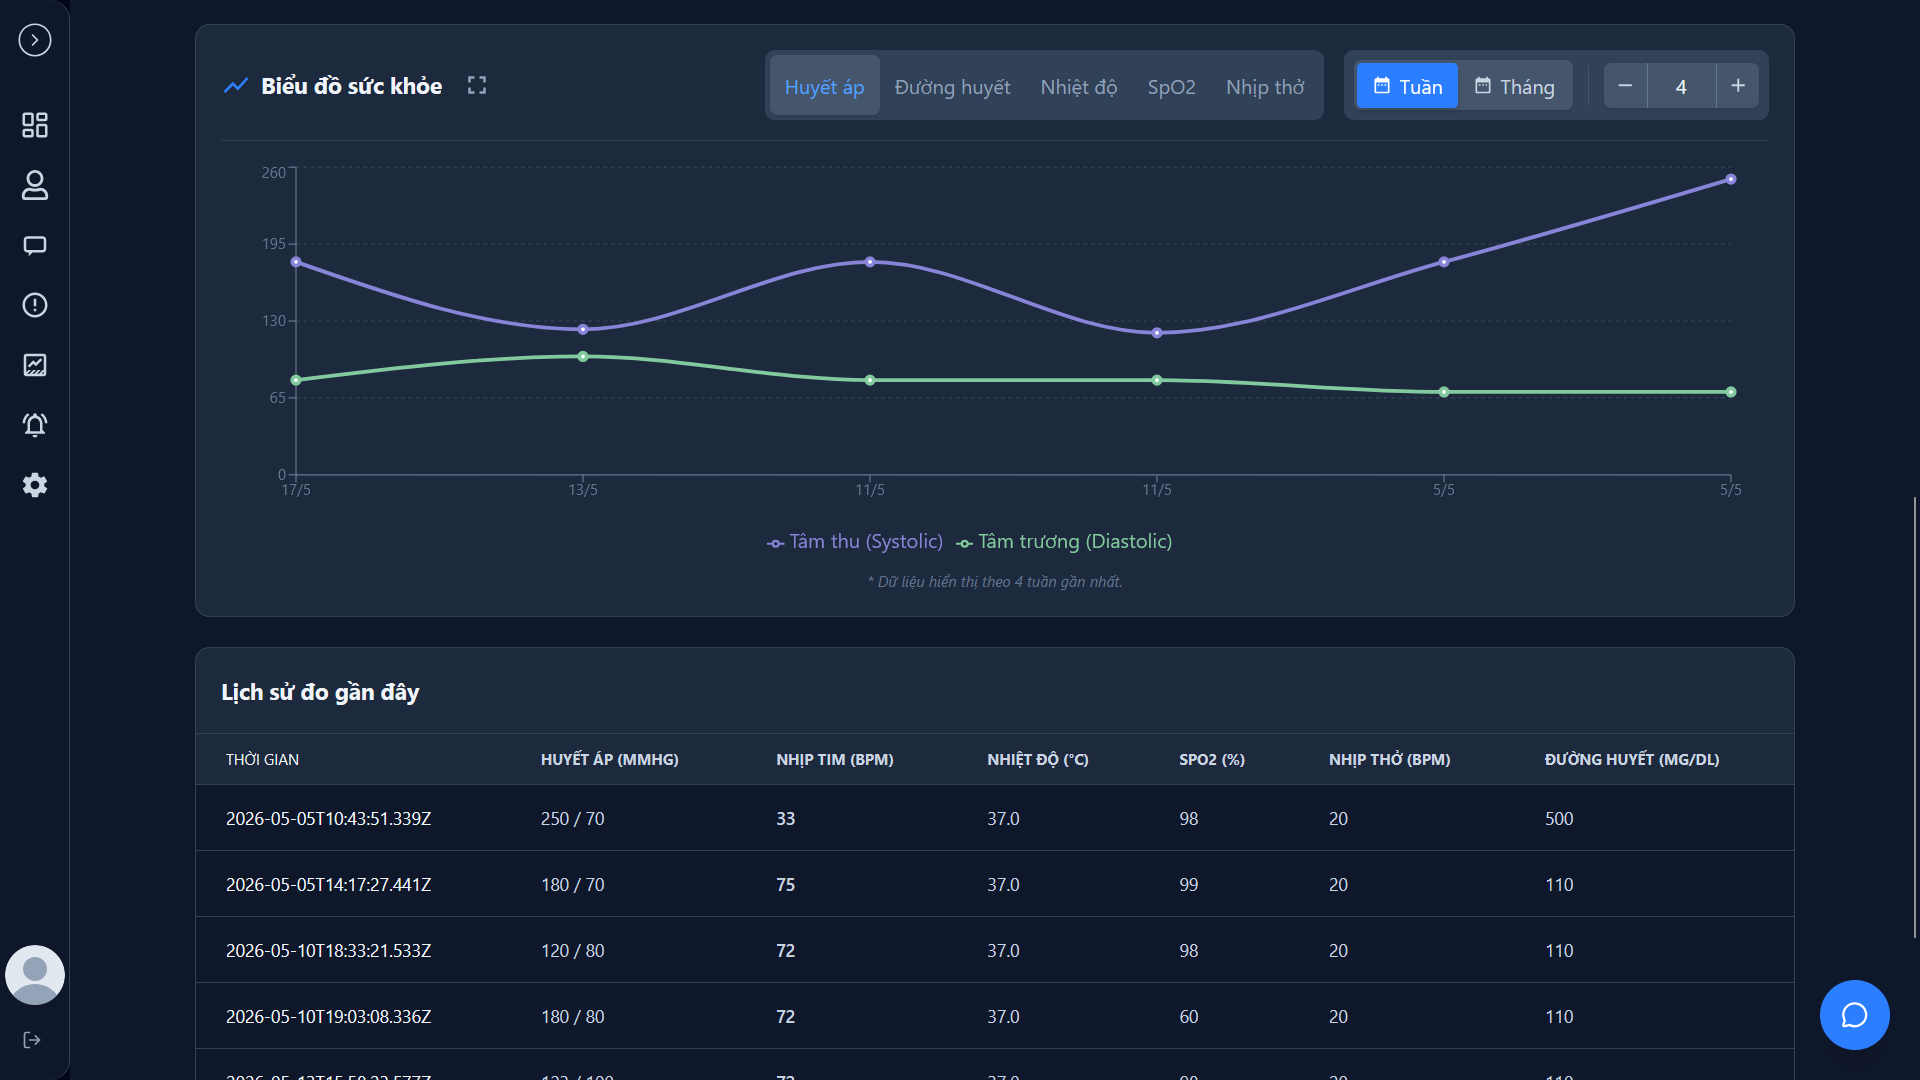
\includegraphics[width=\textwidth,keepaspectratio]{images/Chapter5/Web/web-patient-detail-charts.png}
    \end{center}
    \caption{\textit{Màn hình biểu đồ xu hướng và lịch sử đo của bệnh nhân}}
    \label{chapter5-image16}
    \end{figure}
\end{center}

\subsubsection{Cấu hình ngưỡng an toàn}
\par Hệ thống cung cấp chức năng cấu hình ngưỡng an toàn cho từng bệnh nhân. Bác sĩ có thể thiết lập các khoảng giá trị tối thiểu và tối đa cho các chỉ số như thân nhiệt, nhịp tim, nhịp thở, SpO2, huyết áp tâm thu, huyết áp tâm trương và đường huyết. Các ngưỡng này được lưu lại trong hệ thống và được sử dụng khi backend đánh giá các lần đo mới của bệnh nhân.

\par Việc cho phép bác sĩ cấu hình ngưỡng theo từng bệnh nhân giúp hệ thống linh hoạt hơn so với việc chỉ dùng một bộ ngưỡng cố định cho toàn bộ người dùng. Trong thực tế, ngưỡng theo dõi có thể thay đổi tùy theo tình trạng bệnh, mục tiêu điều trị hoặc chỉ định của bác sĩ. Trong phạm vi đồ án, hệ thống chưa sử dụng AI hay học máy để dự đoán rủi ro, nhưng cơ chế ngưỡng do bác sĩ cấu hình là một cách tiếp cận rõ ràng, dễ kiểm soát và phù hợp với yêu cầu Proof-of-Concept.

\begin{center}
    \begin{figure}[H]
    \begin{center}
     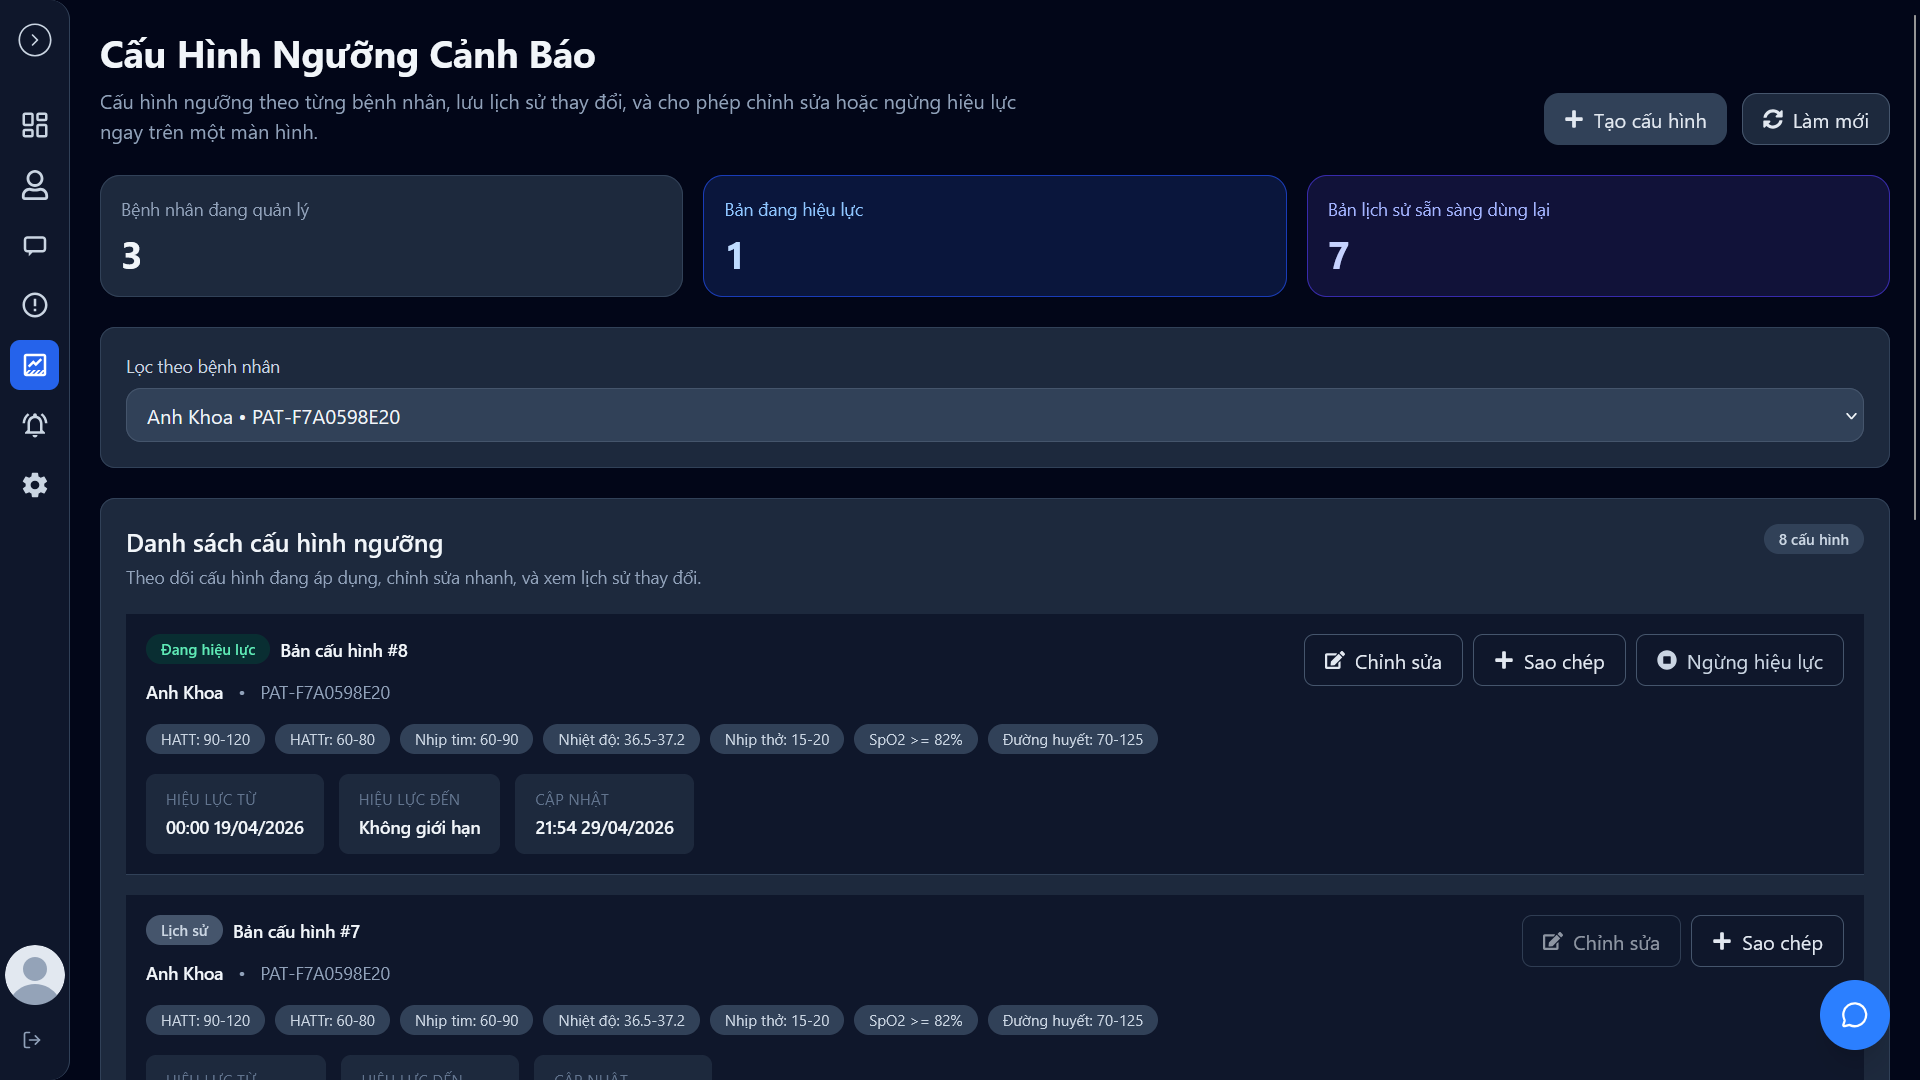
\includegraphics[width=\textwidth,keepaspectratio]{images/Chapter5/Web/web-threshold-settings.png}
     \vspace{0.5cm}
    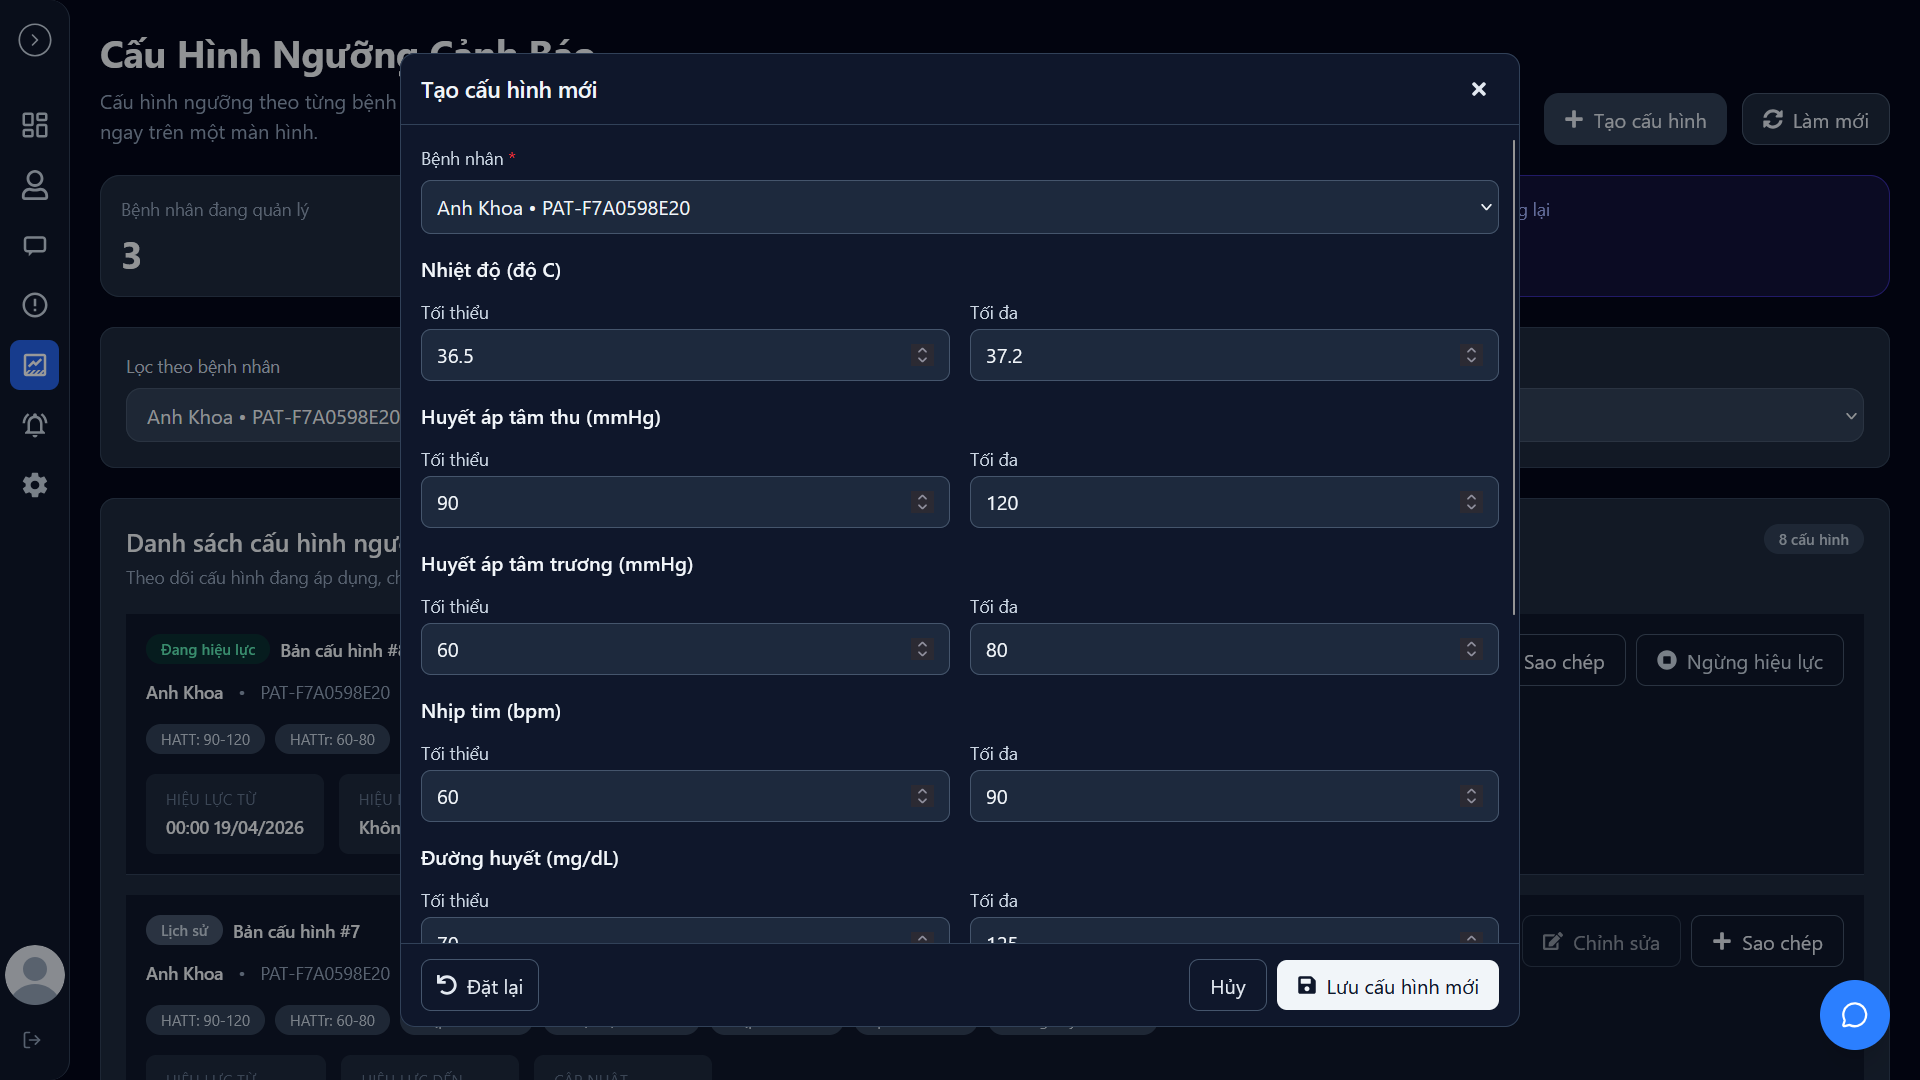
\includegraphics[width=\textwidth,keepaspectratio]{images/Chapter5/Web/web-threshold-settings2.png}
    \end{center}
    \caption{\textit{Màn hình cấu hình ngưỡng an toàn cho bệnh nhân}}
    \label{chapter5-image17}
    \end{figure}
\end{center}

\subsubsection{Quản lý cảnh báo vượt ngưỡng}
\par Màn hình quản lý cảnh báo giúp bác sĩ xem danh sách các cảnh báo được sinh ra khi bệnh nhân nhập chỉ số vượt ngưỡng. Mỗi cảnh báo chứa thông tin bệnh nhân, thời điểm phát sinh, mức độ cảnh báo, trạng thái xử lý và danh sách các chỉ số vi phạm. Bác sĩ có thể lọc hoặc tìm kiếm cảnh báo để ưu tiên xử lý các trường hợp cần chú ý.

\par Khi xem chi tiết một cảnh báo, bác sĩ có thể biết rõ chỉ số nào đã vượt ngưỡng, giá trị đo được là bao nhiêu và ngưỡng tham chiếu là gì. Sau khi xem xét, bác sĩ có thể xác nhận cảnh báo để đánh dấu rằng cảnh báo đã được tiếp nhận hoặc xử lý. Cơ chế này giúp tránh tình trạng một cảnh báo tồn tại mãi ở trạng thái chưa xử lý, đồng thời hỗ trợ quá trình theo dõi trách nhiệm phản hồi của nhân viên y tế.

\begin{center}
    \begin{figure}[H]
    \begin{center}
     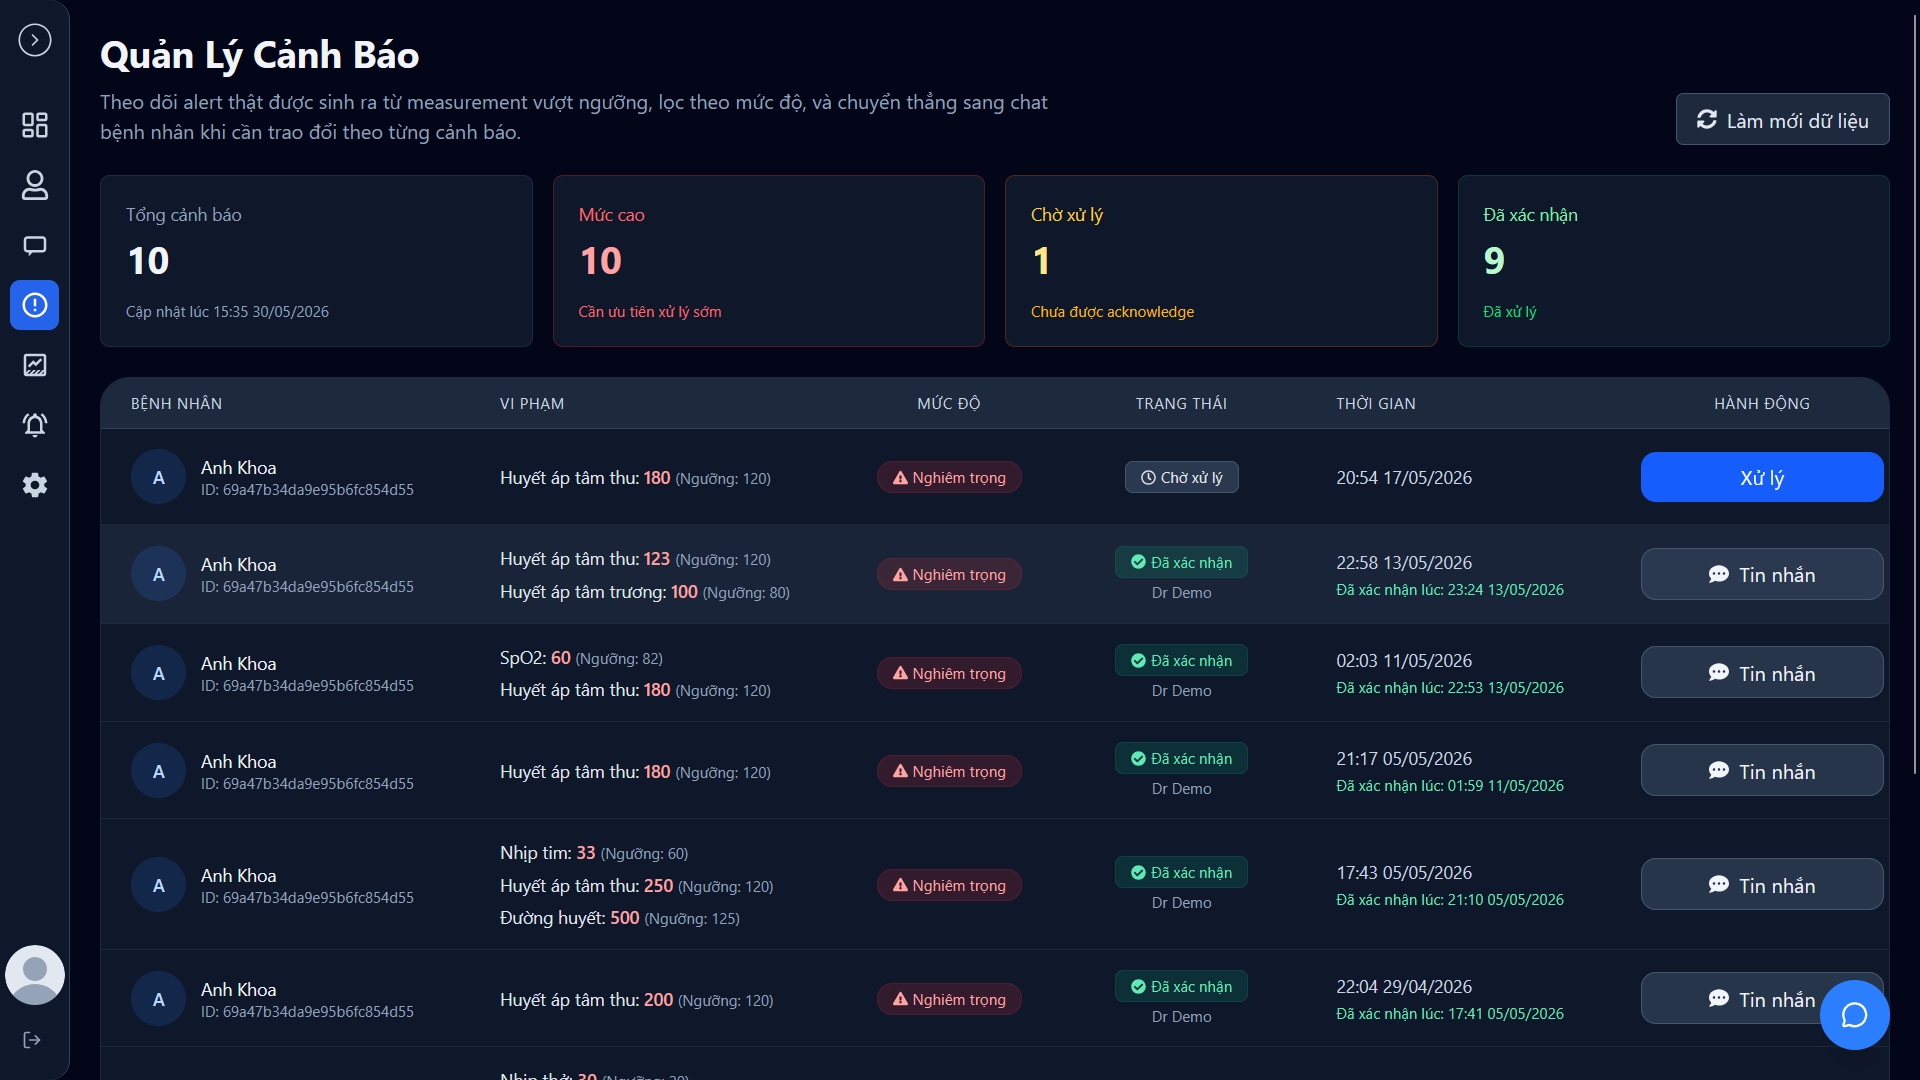
\includegraphics[width=\textwidth,keepaspectratio]{images/Chapter5/Web/web-threshold-alerts.png}
    \end{center}
    \caption{\textit{Màn hình quản lý cảnh báo vượt ngưỡng}}
    \label{chapter5-image18}
    \end{figure}
\end{center}

\subsubsection{Tạo và quản lý nhắc nhở}
\par Trang web dành cho bác sĩ hỗ trợ chức năng tạo nhắc nhở cho bệnh nhân. Nhắc nhở có thể liên quan đến việc đo chỉ số sức khỏe hoặc dùng thuốc. Khi tạo nhắc nhở, bác sĩ chọn bệnh nhân, loại nhắc nhở, nội dung nhắc nhở, thời gian thực hiện, các ngày lặp lại trong tuần, ngày bắt đầu, ngày kết thúc và trạng thái hoạt động. Sau khi được tạo, nhắc nhở được lưu trong hệ thống và được workflow phía backend xử lý để gửi thông báo đúng thời điểm.

\par Màn hình nhắc nhở cũng cho phép bác sĩ lọc danh sách theo bệnh nhân, loại nhắc nhở hoặc trạng thái. Bác sĩ có thể chỉnh sửa nhắc nhở, tạm dừng, tiếp tục hoặc hủy nhắc nhở khi kế hoạch chăm sóc thay đổi. Chức năng này giúp hệ thống không chỉ phản ứng khi có dữ liệu bất thường mà còn hỗ trợ chủ động nhắc bệnh nhân thực hiện các thao tác theo dõi cần thiết.

\begin{center}
    \begin{figure}[H]
    \begin{center}
     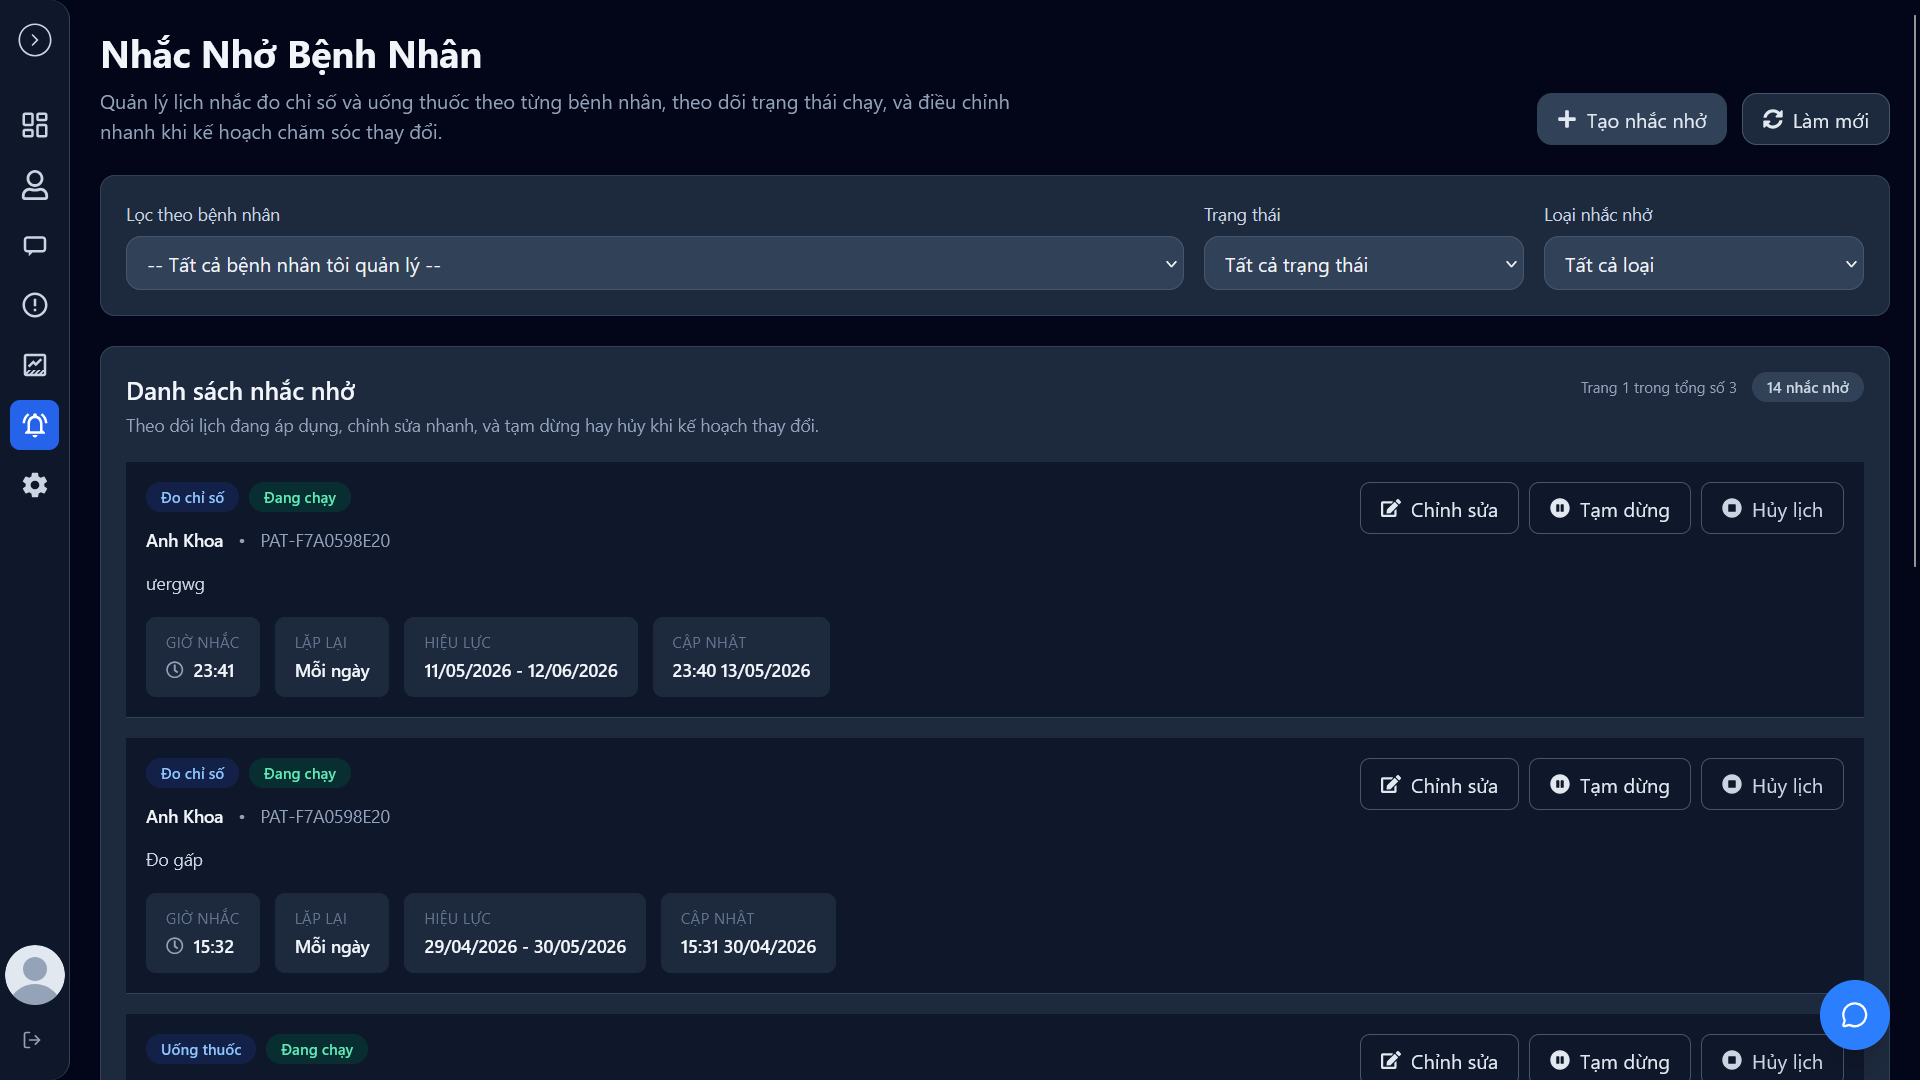
\includegraphics[width=\textwidth,keepaspectratio]{images/Chapter5/Web/web-reminders.png}
    \vspace{0.5cm}
    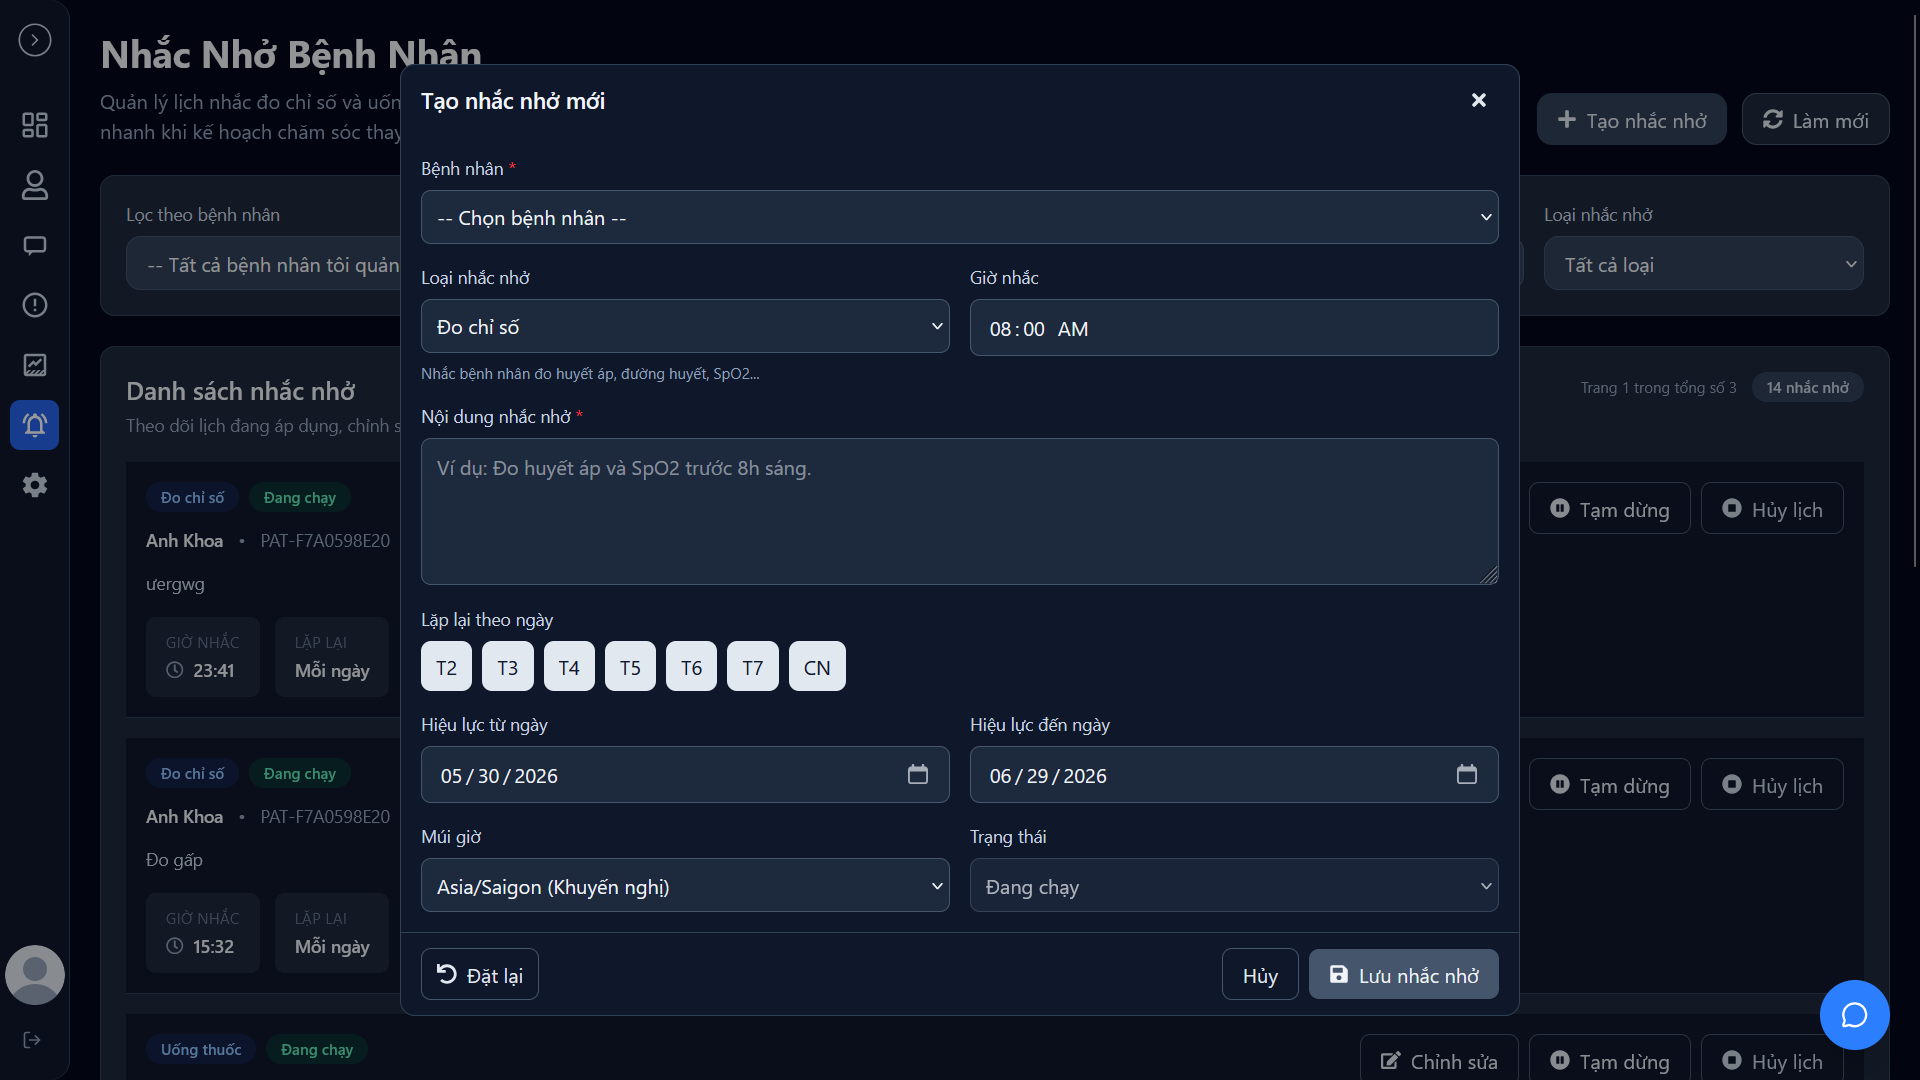
\includegraphics[width=\textwidth,keepaspectratio]{images/Chapter5/Web/web-reminders2.png}
    \end{center}
    \caption{\textit{Màn hình tạo và quản lý nhắc nhở cho bệnh nhân}}
    \label{chapter5-image19}
    \end{figure}
\end{center}

\subsubsection{Danh sách cuộc trò chuyện}
\par Bác sĩ có thể truy cập màn hình danh sách tin nhắn để xem các cuộc trò chuyện với bệnh nhân. Danh sách này hiển thị tên bệnh nhân, nội dung tin nhắn gần nhất, thời điểm cập nhật và trạng thái cuộc trò chuyện nếu có. Bác sĩ có thể tìm kiếm bệnh nhân để mở nhanh cuộc trò chuyện cần xử lý, đặc biệt trong trường hợp có nhiều bệnh nhân được phân công.

\par Chức năng danh sách cuộc trò chuyện giúp bác sĩ không phải mở từng hồ sơ bệnh nhân để kiểm tra tin nhắn. Khi có cảnh báo mới hoặc bệnh nhân gửi tin nhắn, bác sĩ có thể nhanh chóng nhận biết và chuyển đến cuộc hội thoại tương ứng. Đây là một thành phần quan trọng trong trải nghiệm làm việc hằng ngày của bác sĩ trên hệ thống RPM.

\begin{center}
    \begin{figure}[H]
    \begin{center}
     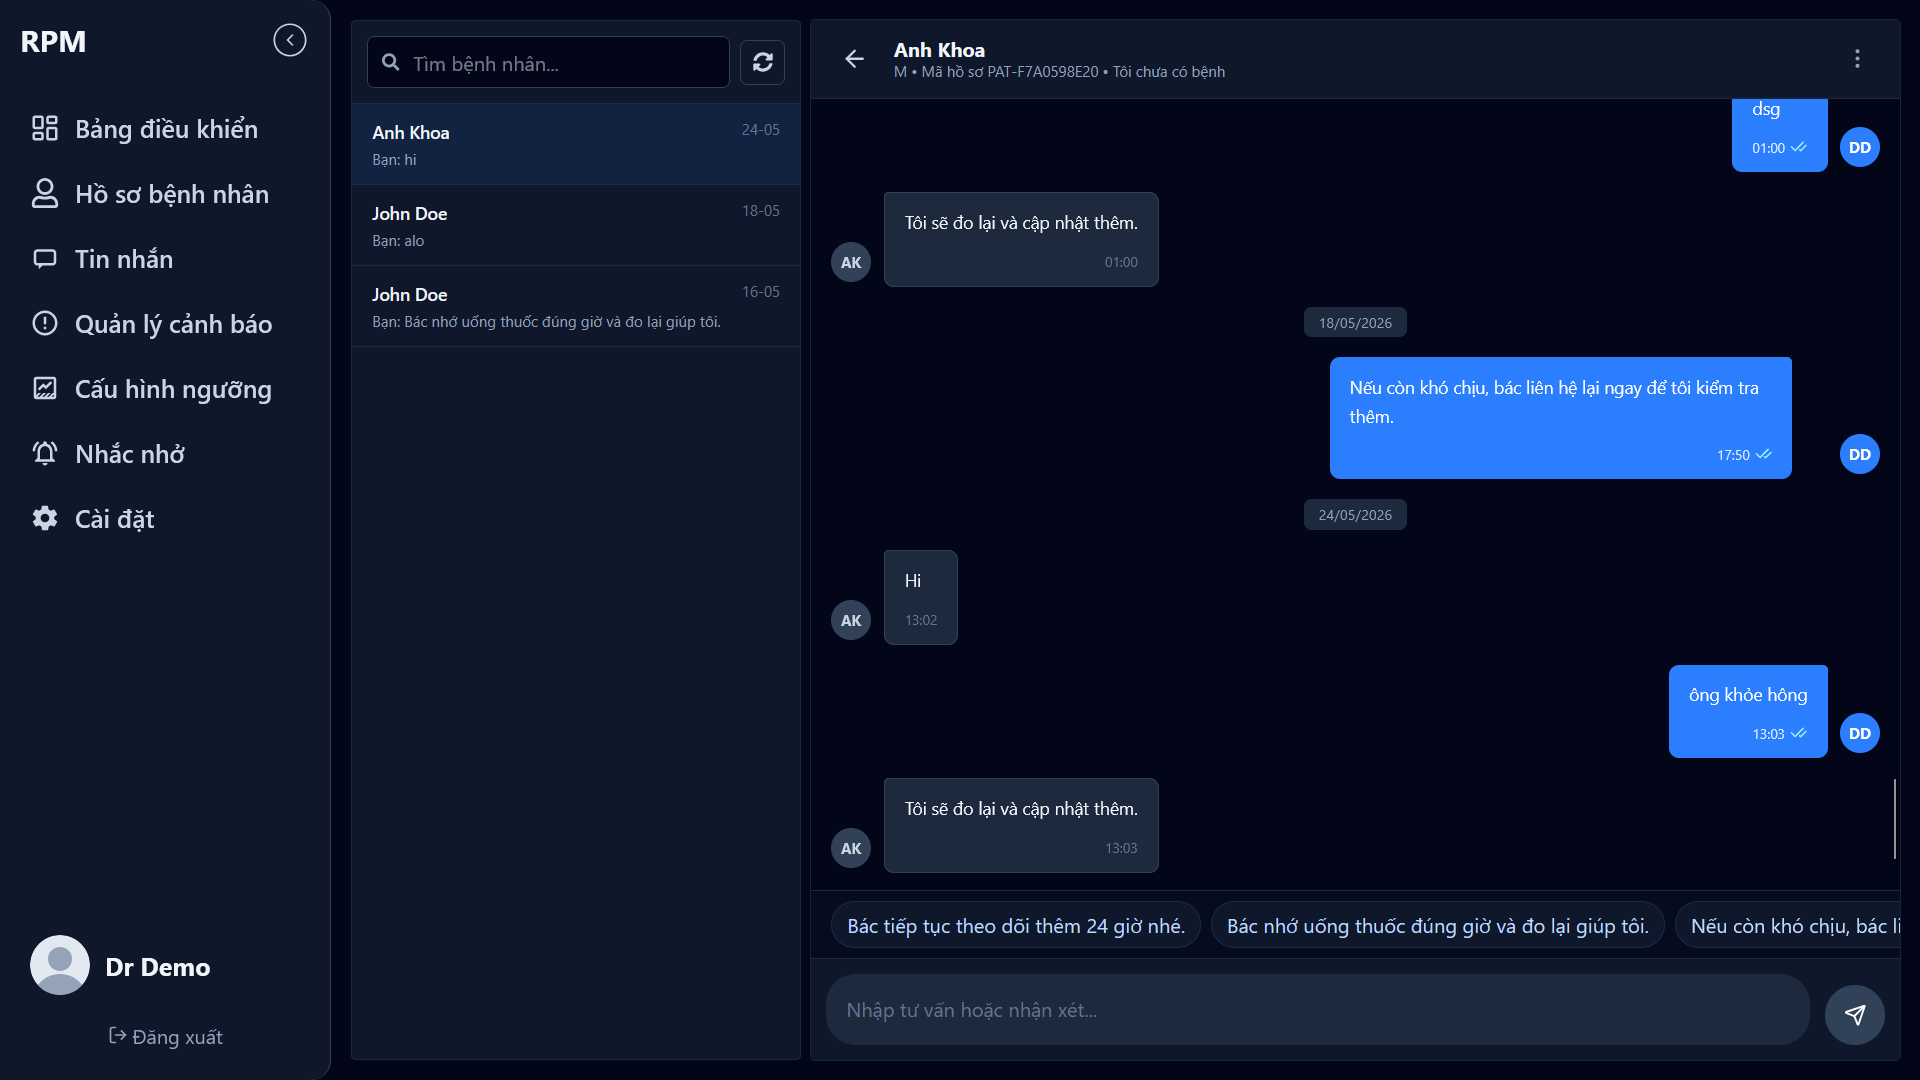
\includegraphics[width=\textwidth,keepaspectratio]{images/Chapter5/Web/web-chat-list.png}
    \end{center}
    \caption{\textit{Màn hình danh sách cuộc trò chuyện giữa bác sĩ và bệnh nhân}}
    \label{chapter5-image20}
    \end{figure}
\end{center}

\subsubsection{Trao đổi tin nhắn và tư vấn trong ngữ cảnh cảnh báo}
\par Màn hình chat chi tiết cho phép bác sĩ trao đổi trực tiếp với bệnh nhân. Bên cạnh tin nhắn thông thường, hệ thống còn hỗ trợ tin nhắn có liên kết với cảnh báo. Khi bác sĩ mở cuộc trò chuyện từ một cảnh báo cụ thể, màn hình chat có thể hiển thị ngữ cảnh cảnh báo, bao gồm mức độ cảnh báo, trạng thái xác nhận, thời điểm đo và danh sách chỉ số vượt ngưỡng. Điều này giúp bác sĩ tư vấn cho bệnh nhân dựa trên thông tin cụ thể thay vì phải quay lại màn hình cảnh báo để kiểm tra.

\par Ngoài ra, hệ thống có thể cung cấp các mẫu tin nhắn nhanh để bác sĩ phản hồi bệnh nhân thuận tiện hơn. Ví dụ, bác sĩ có thể nhắc bệnh nhân tiếp tục theo dõi thêm, đo lại chỉ số hoặc liên hệ khi có triệu chứng bất thường. Chức năng chat không thay thế cho khám chữa bệnh trực tiếp, nhưng đóng vai trò hỗ trợ trao đổi thông tin trong quá trình theo dõi từ xa.

\begin{center}
    \begin{figure}[H]
    \begin{center}
     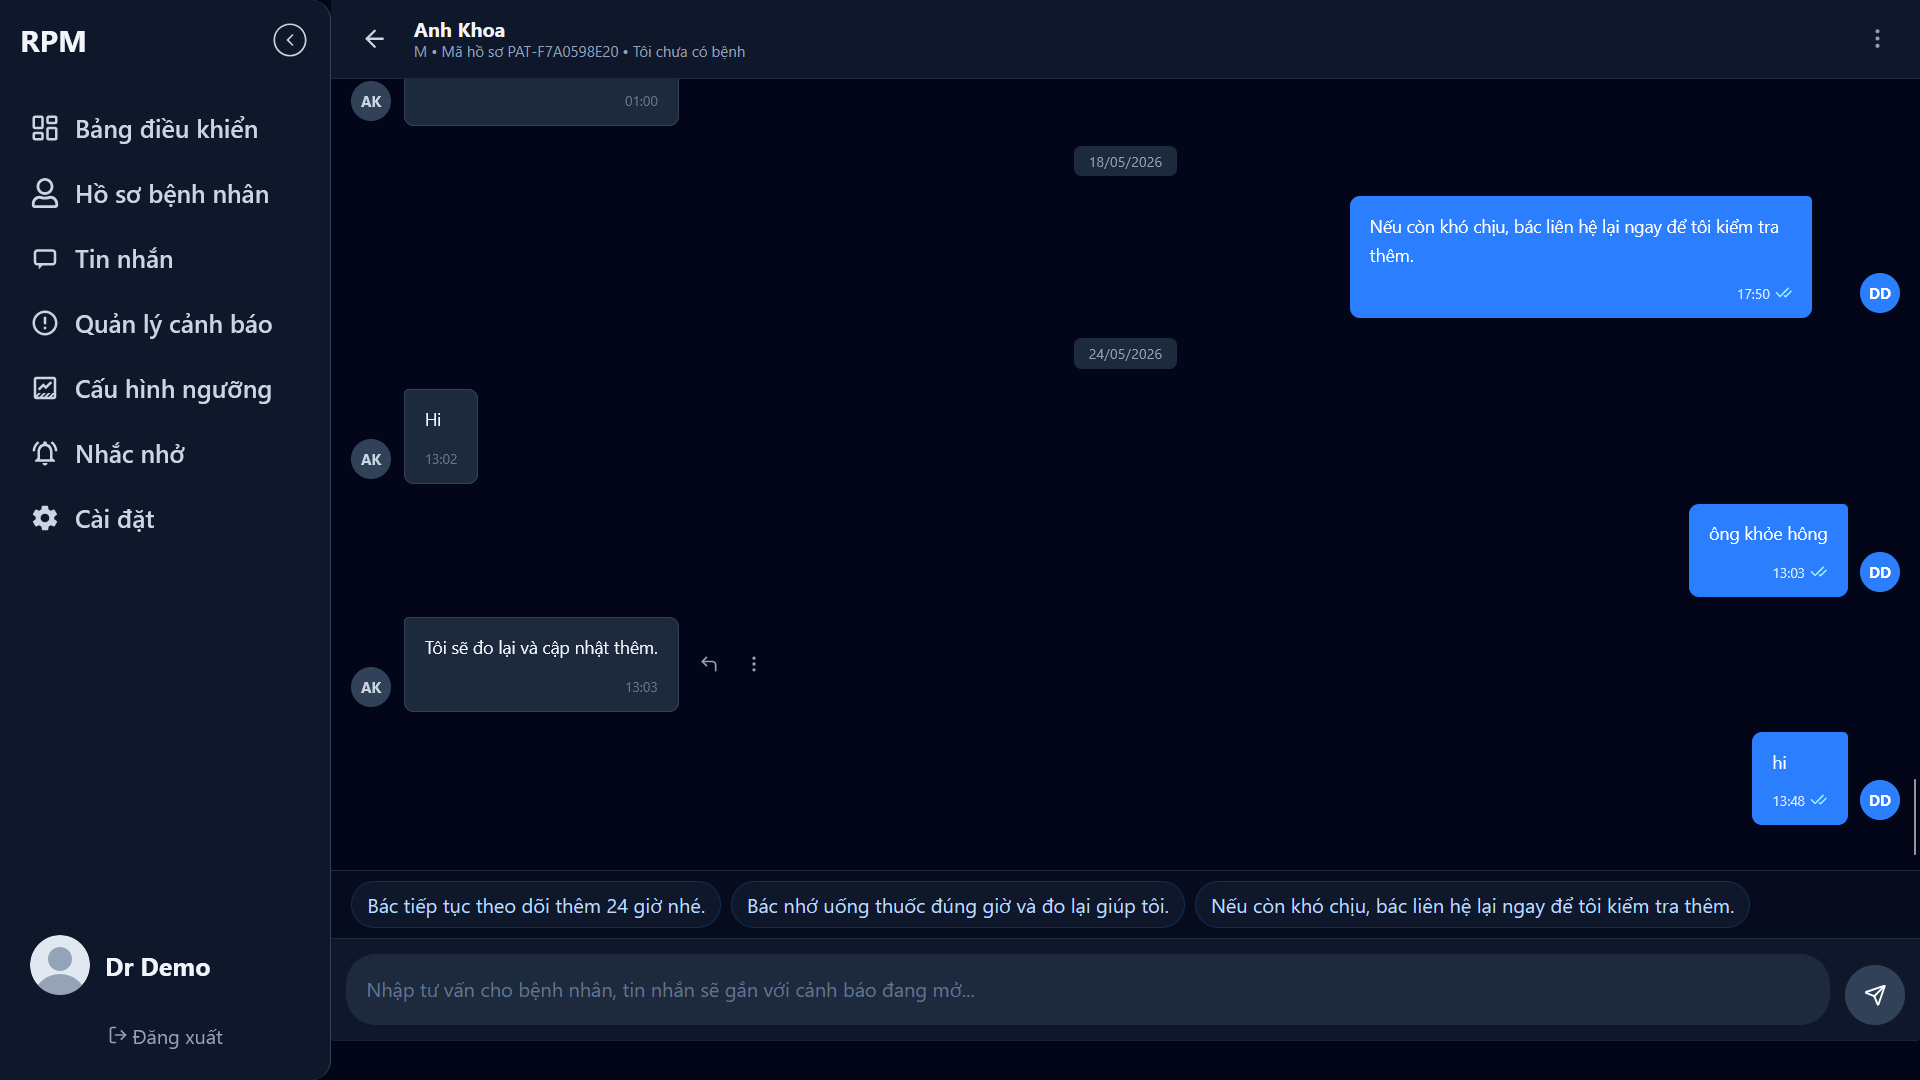
\includegraphics[width=\textwidth,keepaspectratio]{images/Chapter5/Web/web-chat-detail.png}
    \end{center}
    \caption{\textit{Màn hình chat chi tiết giữa bác sĩ và bệnh nhân trong ngữ cảnh cảnh báo}}
    \label{chapter5-image21}
    \end{figure}
\end{center}

\subsubsection{Hồ sơ bác sĩ và cài đặt giao diện}
\par Trang web bác sĩ cung cấp màn hình hồ sơ cá nhân để bác sĩ xem thông tin của mình, bao gồm họ tên, giới tính, ngày sinh, email, số điện thoại, chuyên khoa, khoa phòng, nơi làm việc, số giấy phép hành nghề và số năm kinh nghiệm. Việc hiển thị hồ sơ giúp bác sĩ kiểm tra thông tin chuyên môn đang được lưu trong hệ thống và đảm bảo tính nhất quán với dữ liệu quản trị.

\par Ngoài hồ sơ cá nhân, hệ thống cũng có màn hình cài đặt giao diện. Bác sĩ có thể tùy chỉnh theme sáng/tối, kiểu chữ và kích thước chữ. Chức năng này tuy không phải nghiệp vụ y tế chính, nhưng giúp cải thiện trải nghiệm sử dụng, đặc biệt khi bác sĩ cần theo dõi nhiều dữ liệu trên màn hình trong thời gian dài.

\begin{center}
    \begin{figure}[H]
    \begin{center}
     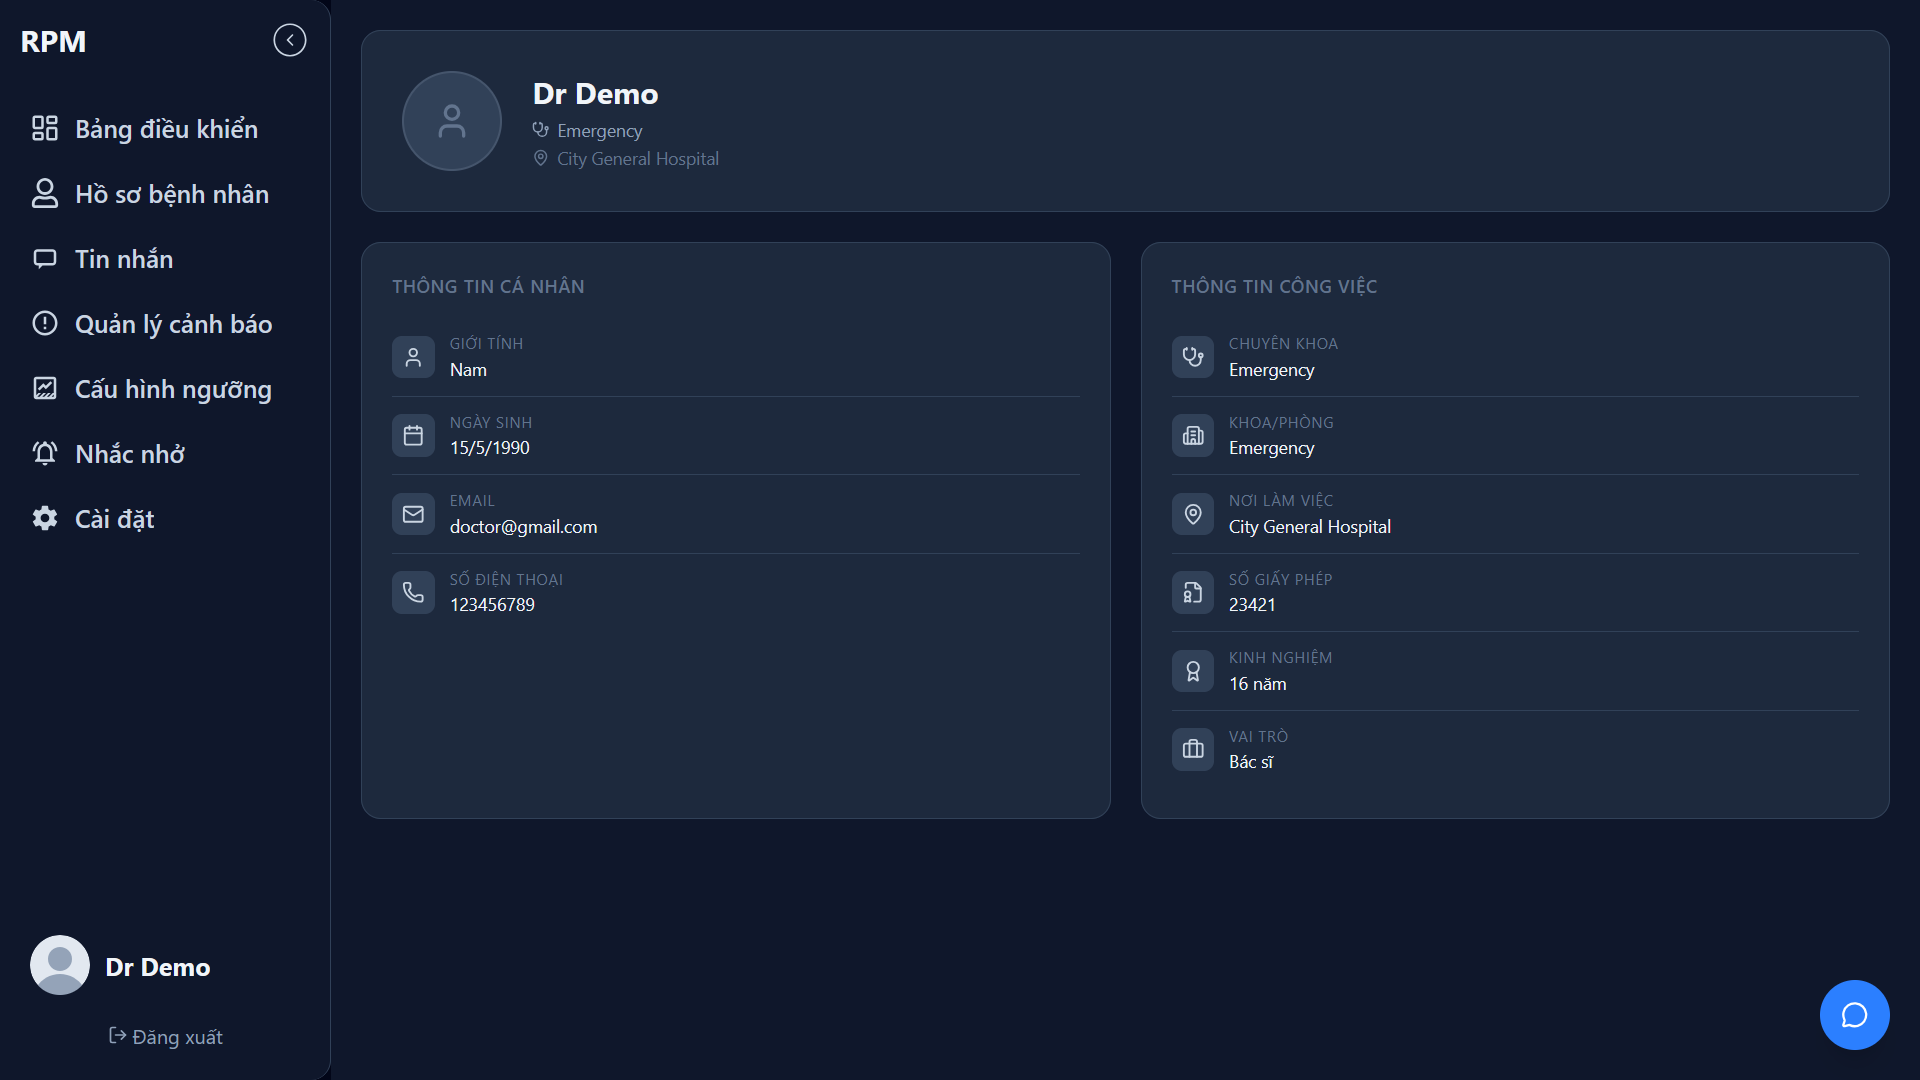
\includegraphics[width=\textwidth,keepaspectratio]{images/Chapter5/Web/web-doctor-profile-settings.png}
    \vspace{0.5cm}
    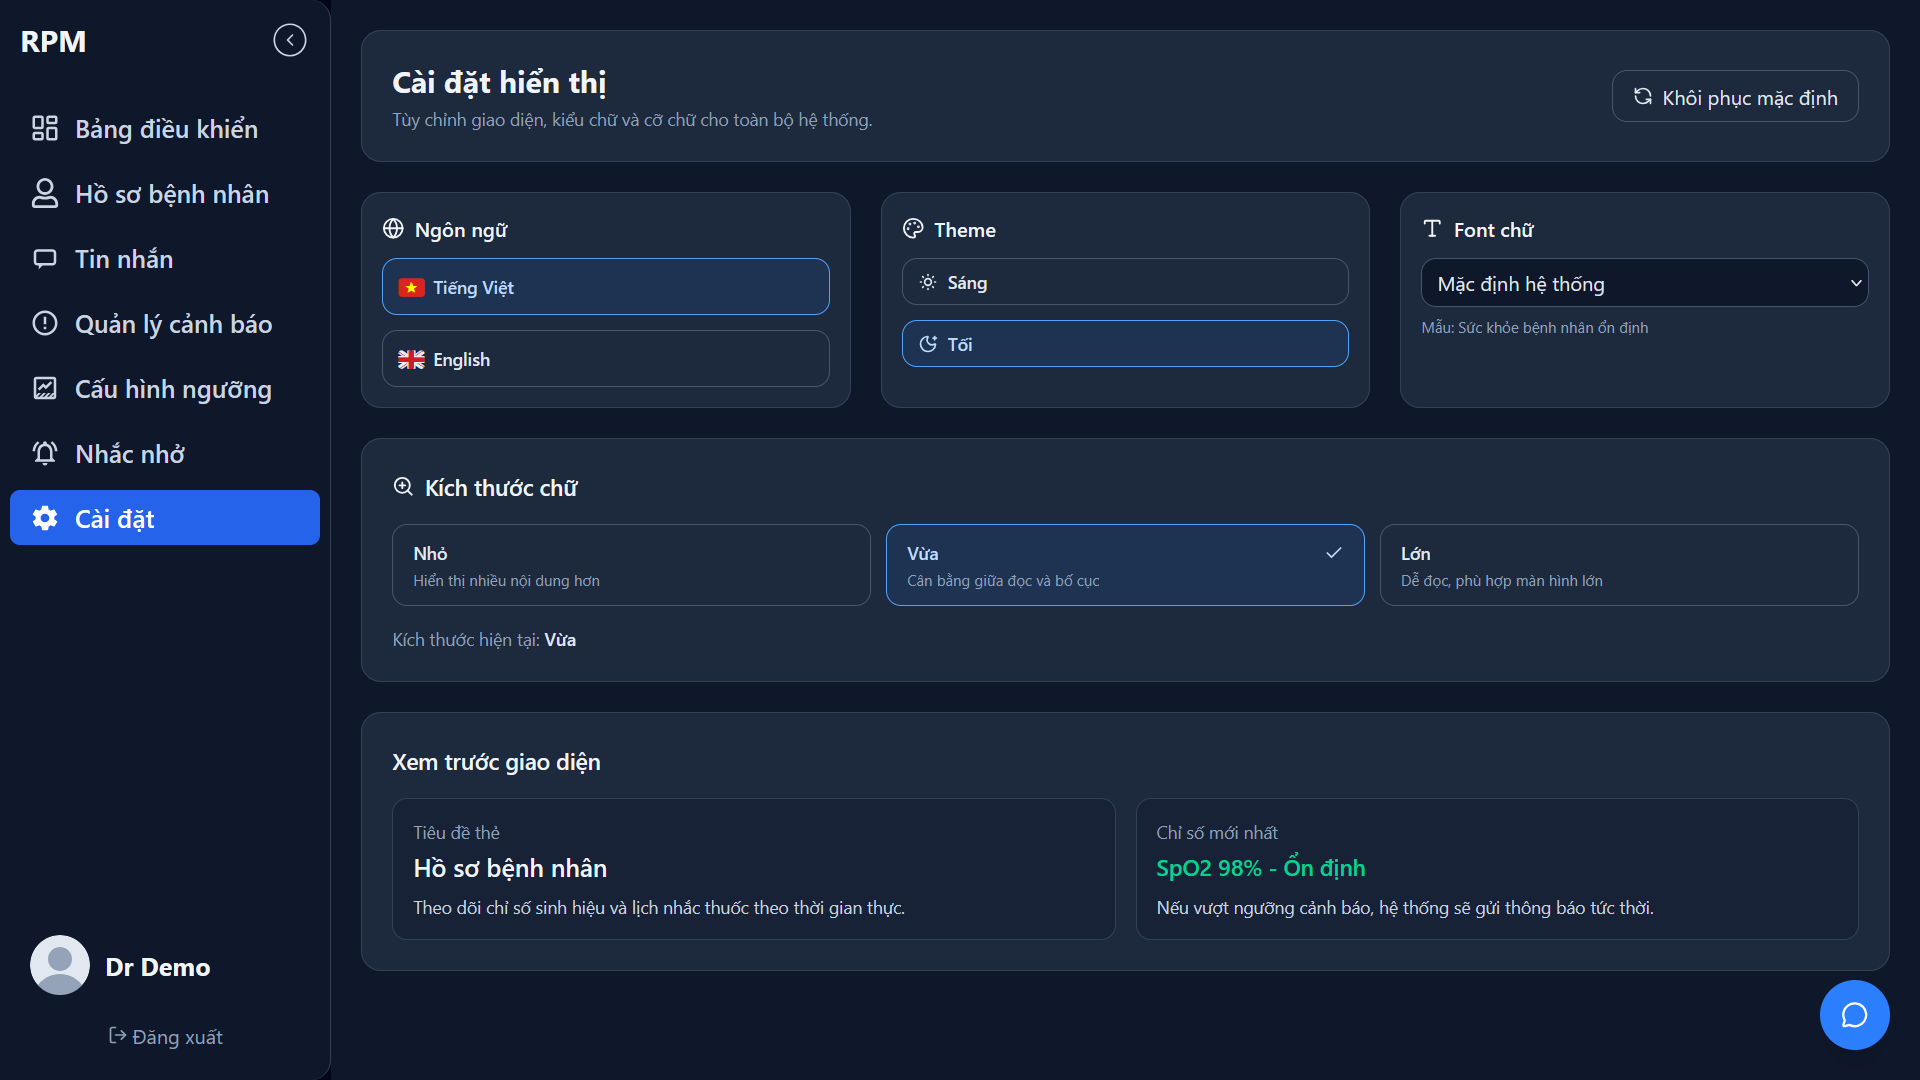
\includegraphics[width=\textwidth,keepaspectratio]{images/Chapter5/Web/web-doctor-profile-settings1.png}
    \end{center}
    \caption{\textit{Màn hình hồ sơ bác sĩ và cài đặt giao diện}}
    \label{chapter5-image22}
    \end{figure}
\end{center}

\newpage
\subsection{Trang web dành cho quản trị viên}

\par Trang web quản trị được xây dựng để hỗ trợ quản trị viên vận hành hệ thống. Nếu trang web bác sĩ tập trung vào nghiệp vụ theo dõi bệnh nhân, thì trang quản trị tập trung vào quản lý tài khoản, khoa phòng, phân công và lịch sử hoạt động. Việc tách riêng trang quản trị giúp phân quyền rõ ràng hơn, tránh để bác sĩ hoặc y tá truy cập các chức năng vận hành không thuộc phạm vi chuyên môn.

\subsubsection{Dashboard quản trị}
\par Dashboard quản trị cung cấp cái nhìn tổng quan về trạng thái hệ thống. Màn hình này hiển thị số lượng bác sĩ, bệnh nhân, y tá và trạng thái hệ thống. Các thẻ thống kê được liên kết đến các màn hình quản lý tương ứng, giúp quản trị viên truy cập nhanh khi cần kiểm tra hoặc cập nhật dữ liệu.

\par Ngoài các số liệu tổng quan, dashboard còn hiển thị danh sách hoạt động gần đây trong hệ thống. Các hoạt động này có thể bao gồm đăng nhập, tạo mới, cập nhật, xóa dữ liệu hoặc các sự kiện hệ thống. Việc hiển thị hoạt động gần đây giúp quản trị viên theo dõi nhanh những thay đổi quan trọng mà không cần mở toàn bộ trang lịch sử hoạt động.

\begin{center}
    \begin{figure}[H]
    \begin{center}
     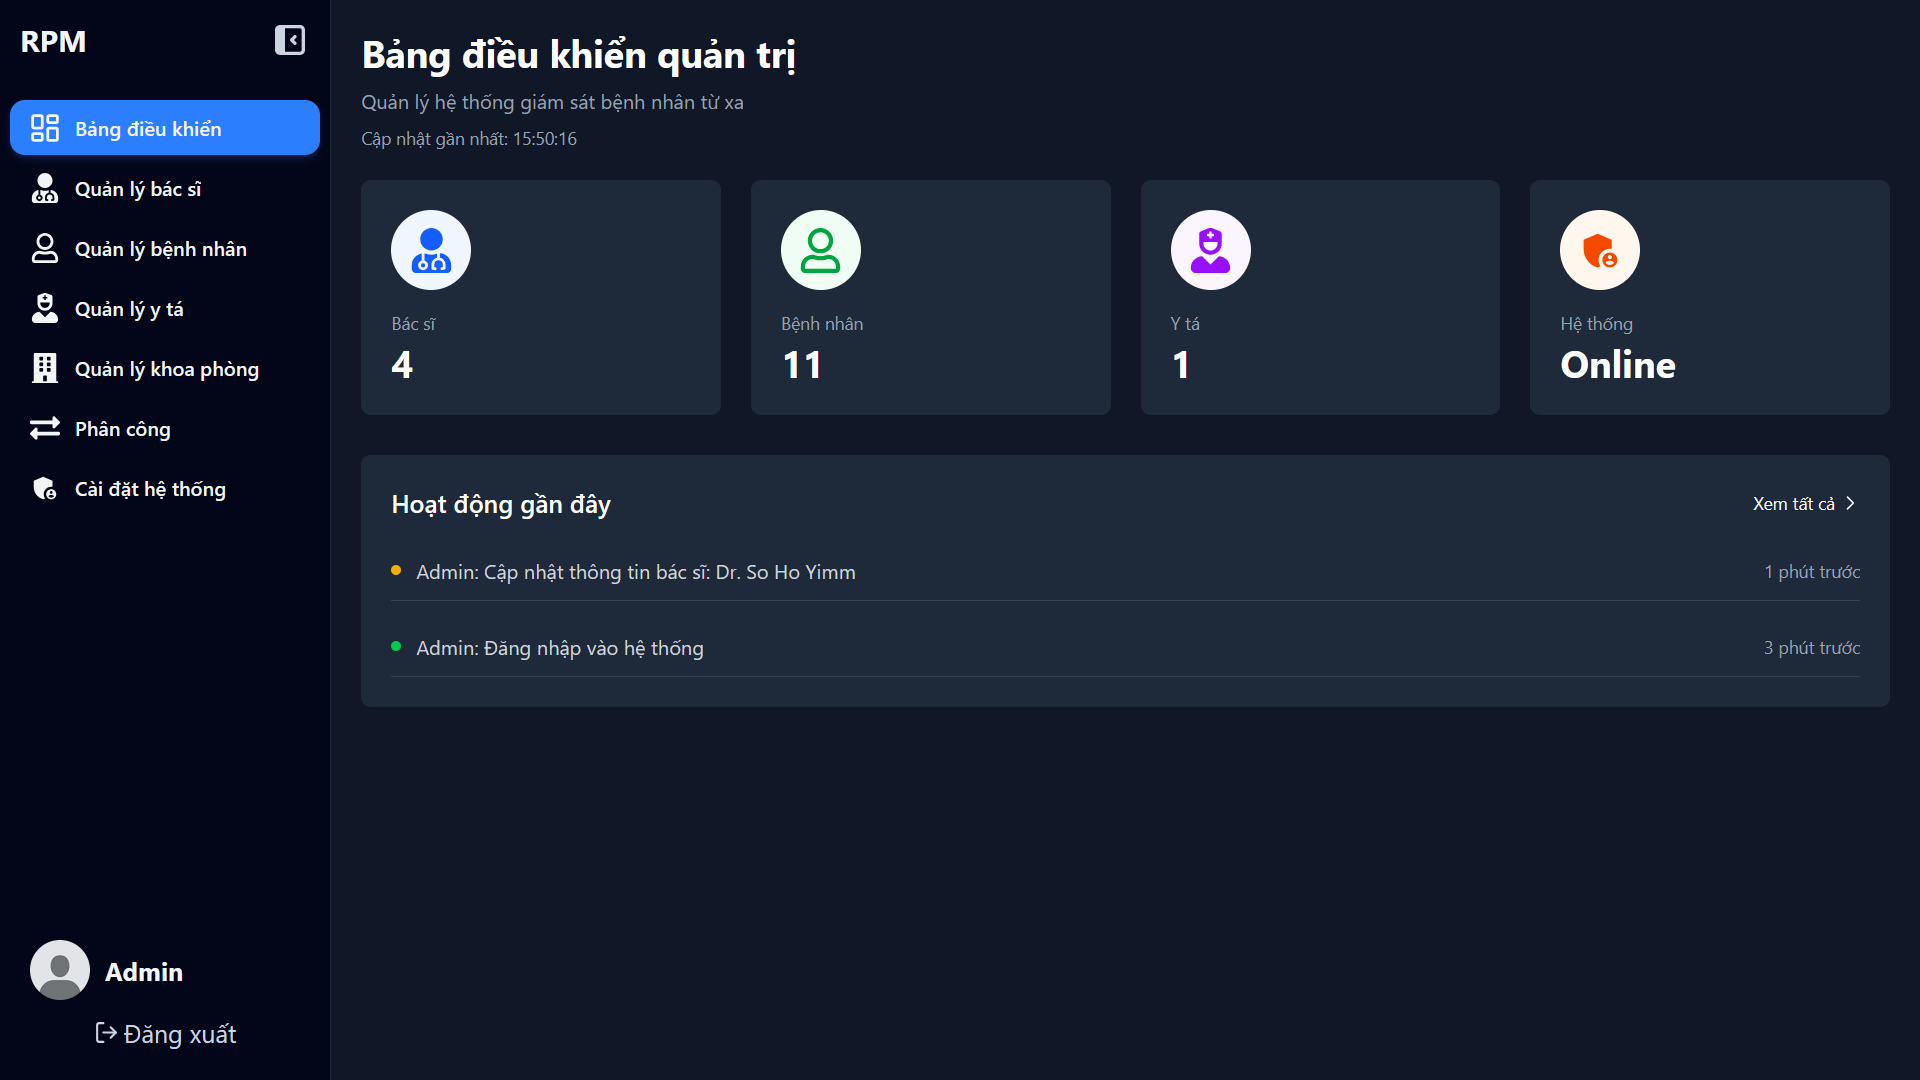
\includegraphics[width=\textwidth,keepaspectratio]{images/Chapter5/Admin/admin-dashboard.png}
    \end{center}
    \caption{\textit{Màn hình dashboard quản trị hệ thống}}
    \label{chapter5-image23}
    \end{figure}
\end{center}

\subsubsection{Quản lý bác sĩ}
\par Chức năng quản lý bác sĩ cho phép quản trị viên xem danh sách bác sĩ trong hệ thống, tìm kiếm theo tên hoặc các thông tin liên quan, thêm bác sĩ mới, cập nhật thông tin bác sĩ và thay đổi trạng thái tài khoản. Thông tin bác sĩ bao gồm họ tên, email, số điện thoại, giới tính, ngày sinh, chuyên khoa, khoa phòng, nơi làm việc, số giấy phép hành nghề, số năm kinh nghiệm và trạng thái tài khoản.

\par Việc quản lý bác sĩ trên trang admin giúp hệ thống đảm bảo dữ liệu nhân sự y tế được lưu trữ có tổ chức. Bác sĩ sau khi được tạo hoặc cập nhật có thể được phân công phụ trách bệnh nhân ở màn hình phân công. Dữ liệu bác sĩ cũng được sử dụng trong web bác sĩ để hiển thị hồ sơ cá nhân và trong hệ thống chat để xác định người phụ trách bệnh nhân.

\begin{center}
    \begin{figure}[H]
    \begin{center}
     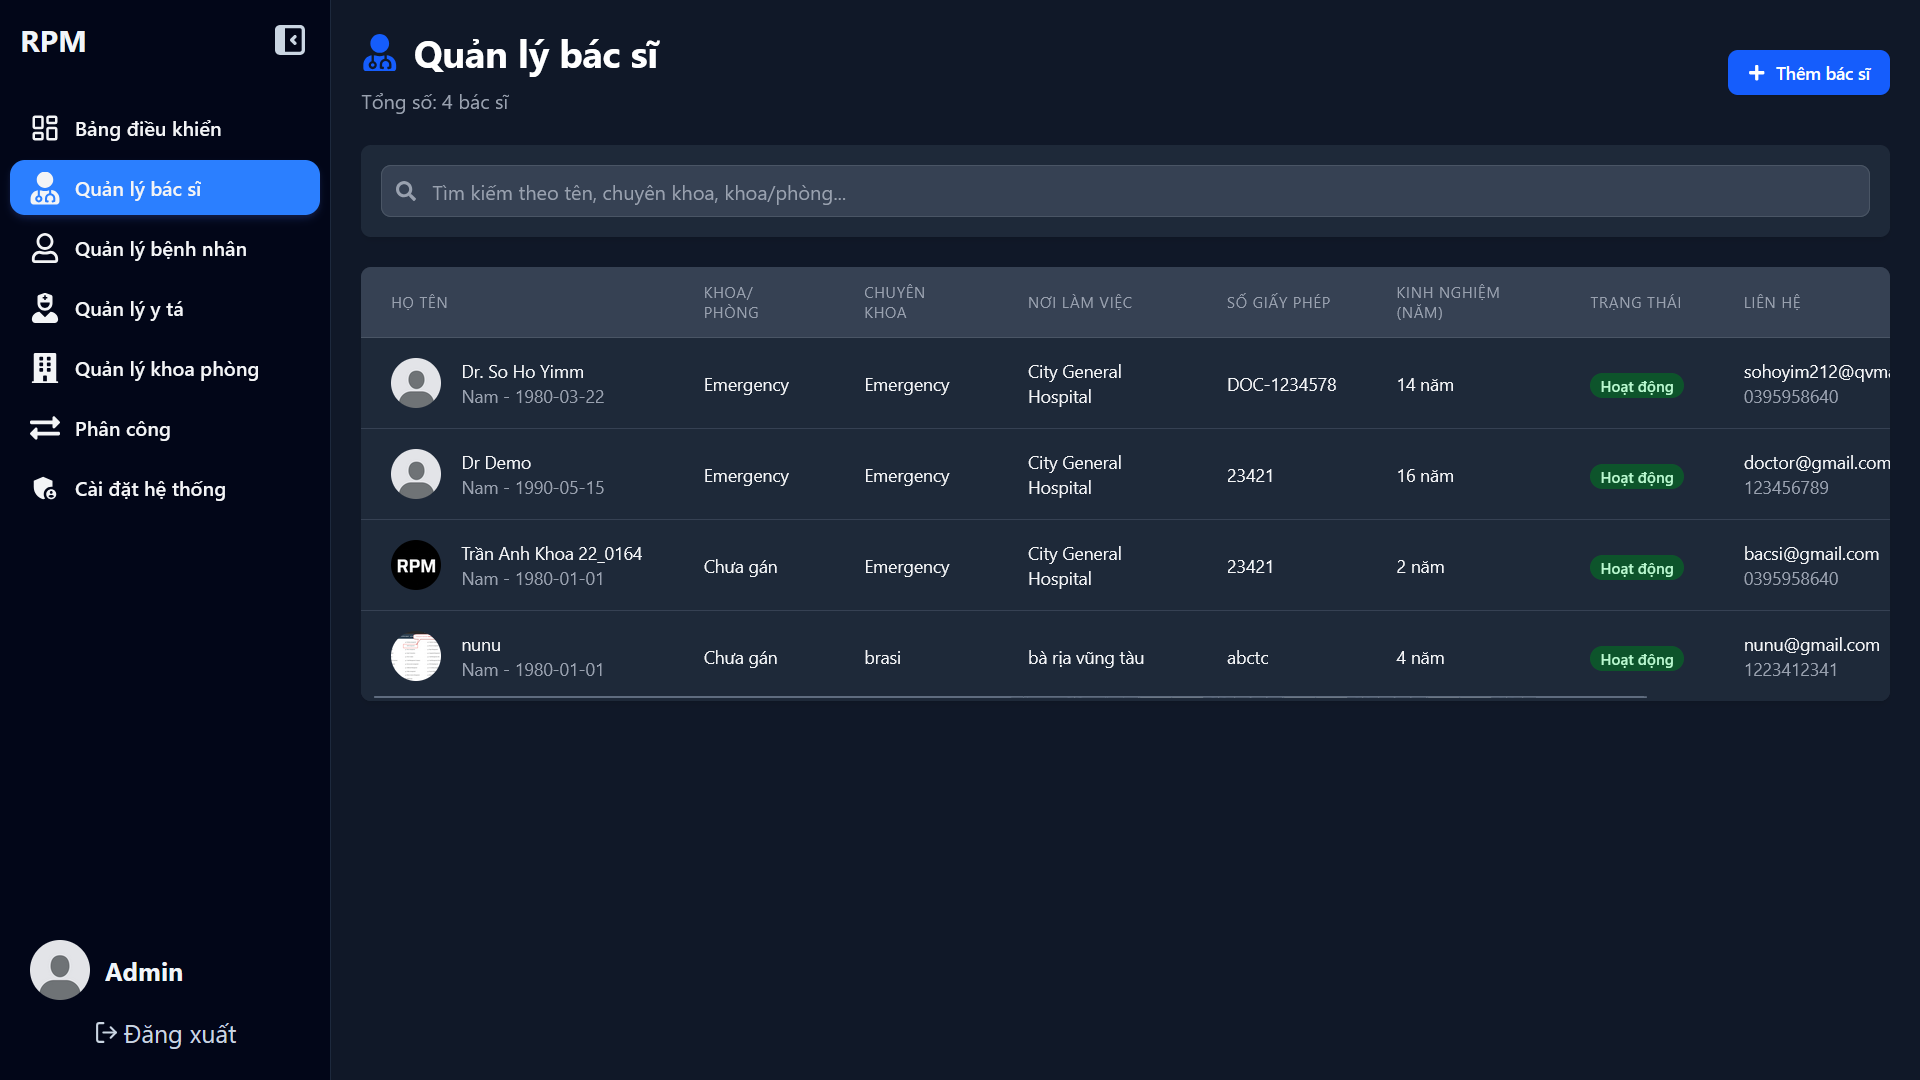
\includegraphics[width=\textwidth,keepaspectratio]{images/Chapter5/Admin/admin-doctor-management.png}
    \end{center}
    \caption{\textit{Màn hình quản lý bác sĩ}}
    \label{chapter5-image24}
    \end{figure}
\end{center}

\subsubsection{Quản lý bệnh nhân}
\par Chức năng quản lý bệnh nhân cho phép quản trị viên xem danh sách bệnh nhân đã có trong hệ thống, thêm bệnh nhân mới, cập nhật thông tin bệnh nhân và xóa hoặc thay đổi trạng thái tài khoản khi cần thiết. Mỗi bệnh nhân có các thông tin cơ bản như họ tên, email, số điện thoại, giới tính, ngày sinh, địa chỉ, trạng thái và ảnh đại diện.

\par Đây là chức năng nền tảng cho toàn bộ hệ thống RPM vì mọi dữ liệu đo, cảnh báo, ngưỡng, nhắc nhở và phân công đều gắn với bệnh nhân. Nếu thông tin bệnh nhân không được quản lý tốt, các chức năng theo dõi phía bác sĩ và y tá sẽ khó hoạt động chính xác. Do đó, trang quản trị đóng vai trò là nơi đảm bảo dữ liệu bệnh nhân được tạo lập và cập nhật đúng trước khi đưa vào quy trình theo dõi.

\begin{center}
    \begin{figure}[H]
    \begin{center}
     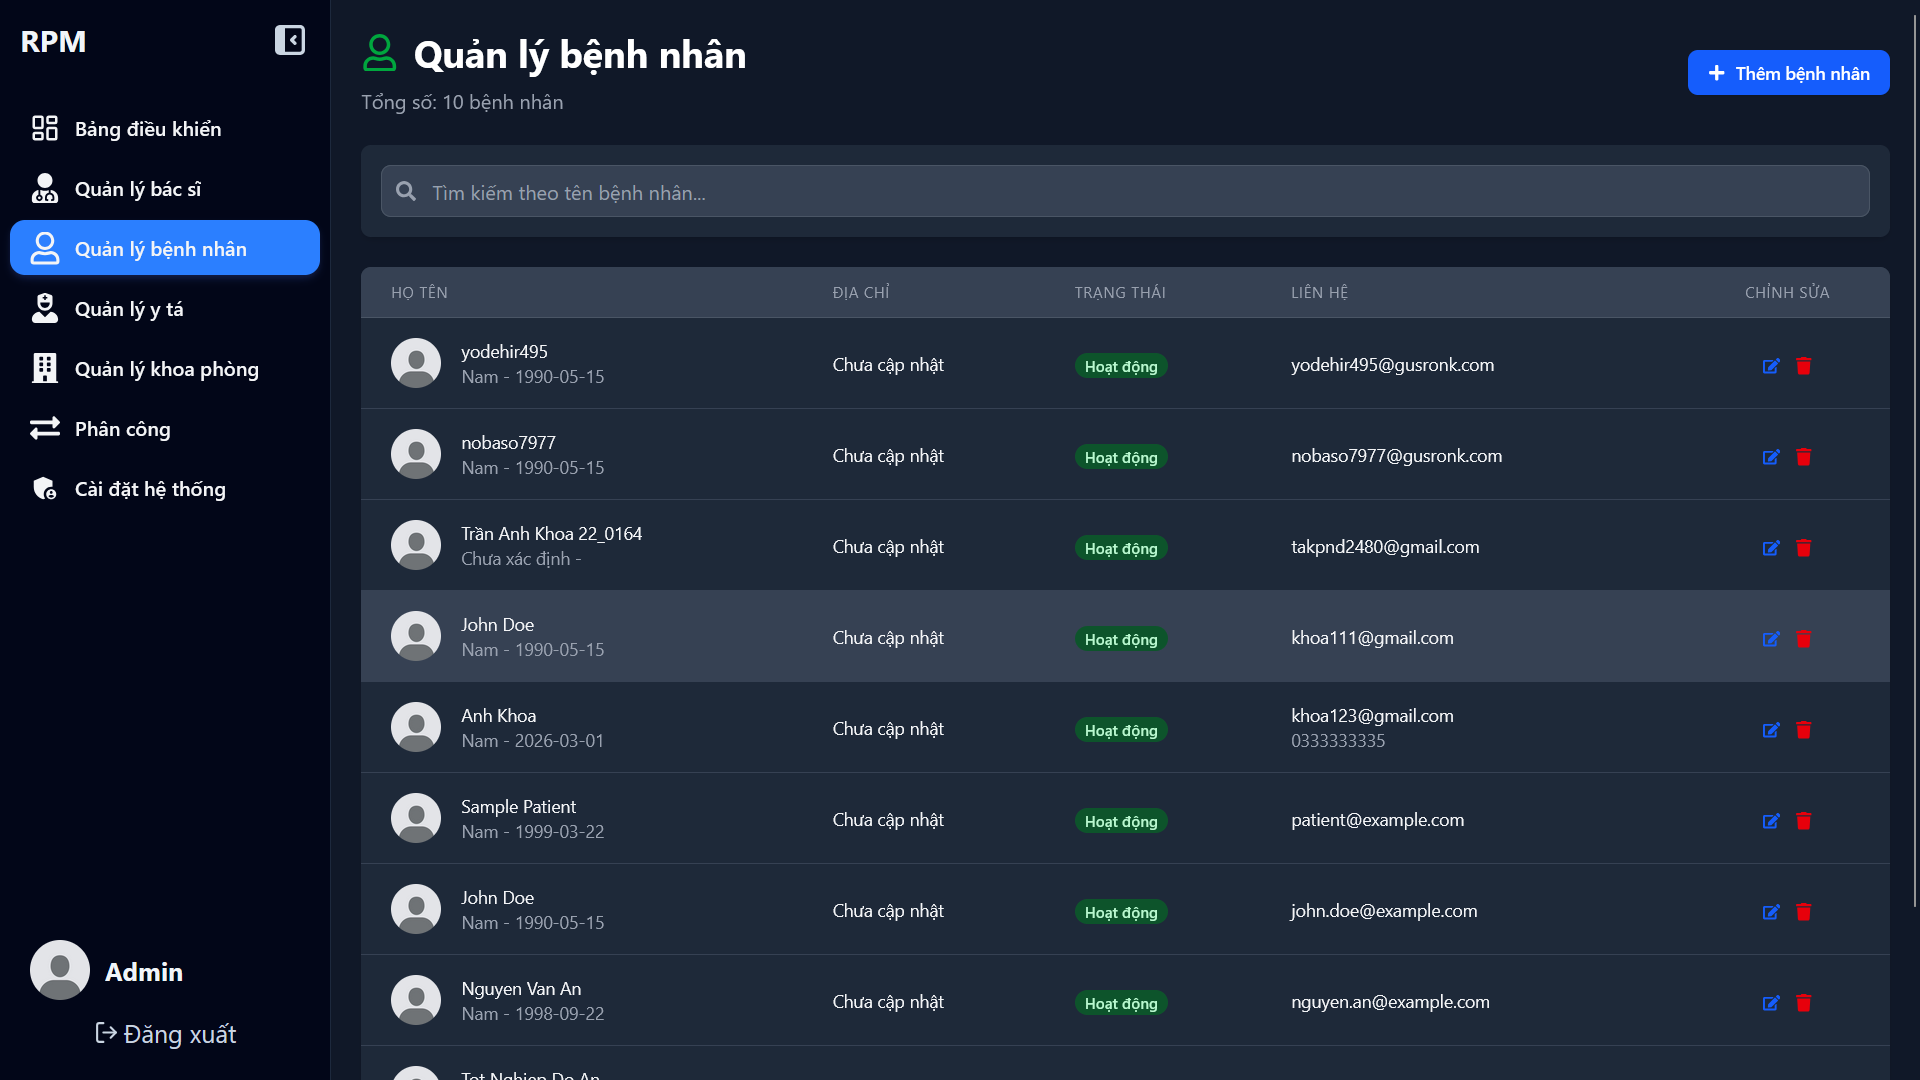
\includegraphics[width=\textwidth,keepaspectratio]{images/Chapter5/Admin/admin-patient-management.png}
    \end{center}
    \caption{\textit{Màn hình quản lý bệnh nhân}}
    \label{chapter5-image25}
    \end{figure}
\end{center}

\subsubsection{Quản lý y tá}
\par Chức năng quản lý y tá cho phép quản trị viên tạo mới, cập nhật, tìm kiếm và quản lý trạng thái tài khoản y tá. Thông tin y tá bao gồm họ tên, email, số điện thoại, giới tính, ngày sinh, khoa phòng, nơi làm việc, số giấy phép hành nghề, số năm kinh nghiệm và trạng thái tài khoản. Dữ liệu này được sử dụng để hiển thị hồ sơ y tá trên ứng dụng di động và để phân công y tá theo dõi bệnh nhân.

\par Việc bổ sung vai trò y tá giúp hệ thống mở rộng hơn so với mô hình chỉ có bệnh nhân và bác sĩ. Trong thực tế, y tá hoặc điều dưỡng thường tham gia vào quá trình đo chỉ số, nhắc nhở bệnh nhân và hỗ trợ bác sĩ theo dõi tình trạng bệnh nhân. Vì vậy, chức năng quản lý y tá giúp hệ thống phản ánh tốt hơn quy trình vận hành của một cơ sở y tế.

\begin{center}
    \begin{figure}[H]
    \begin{center}
     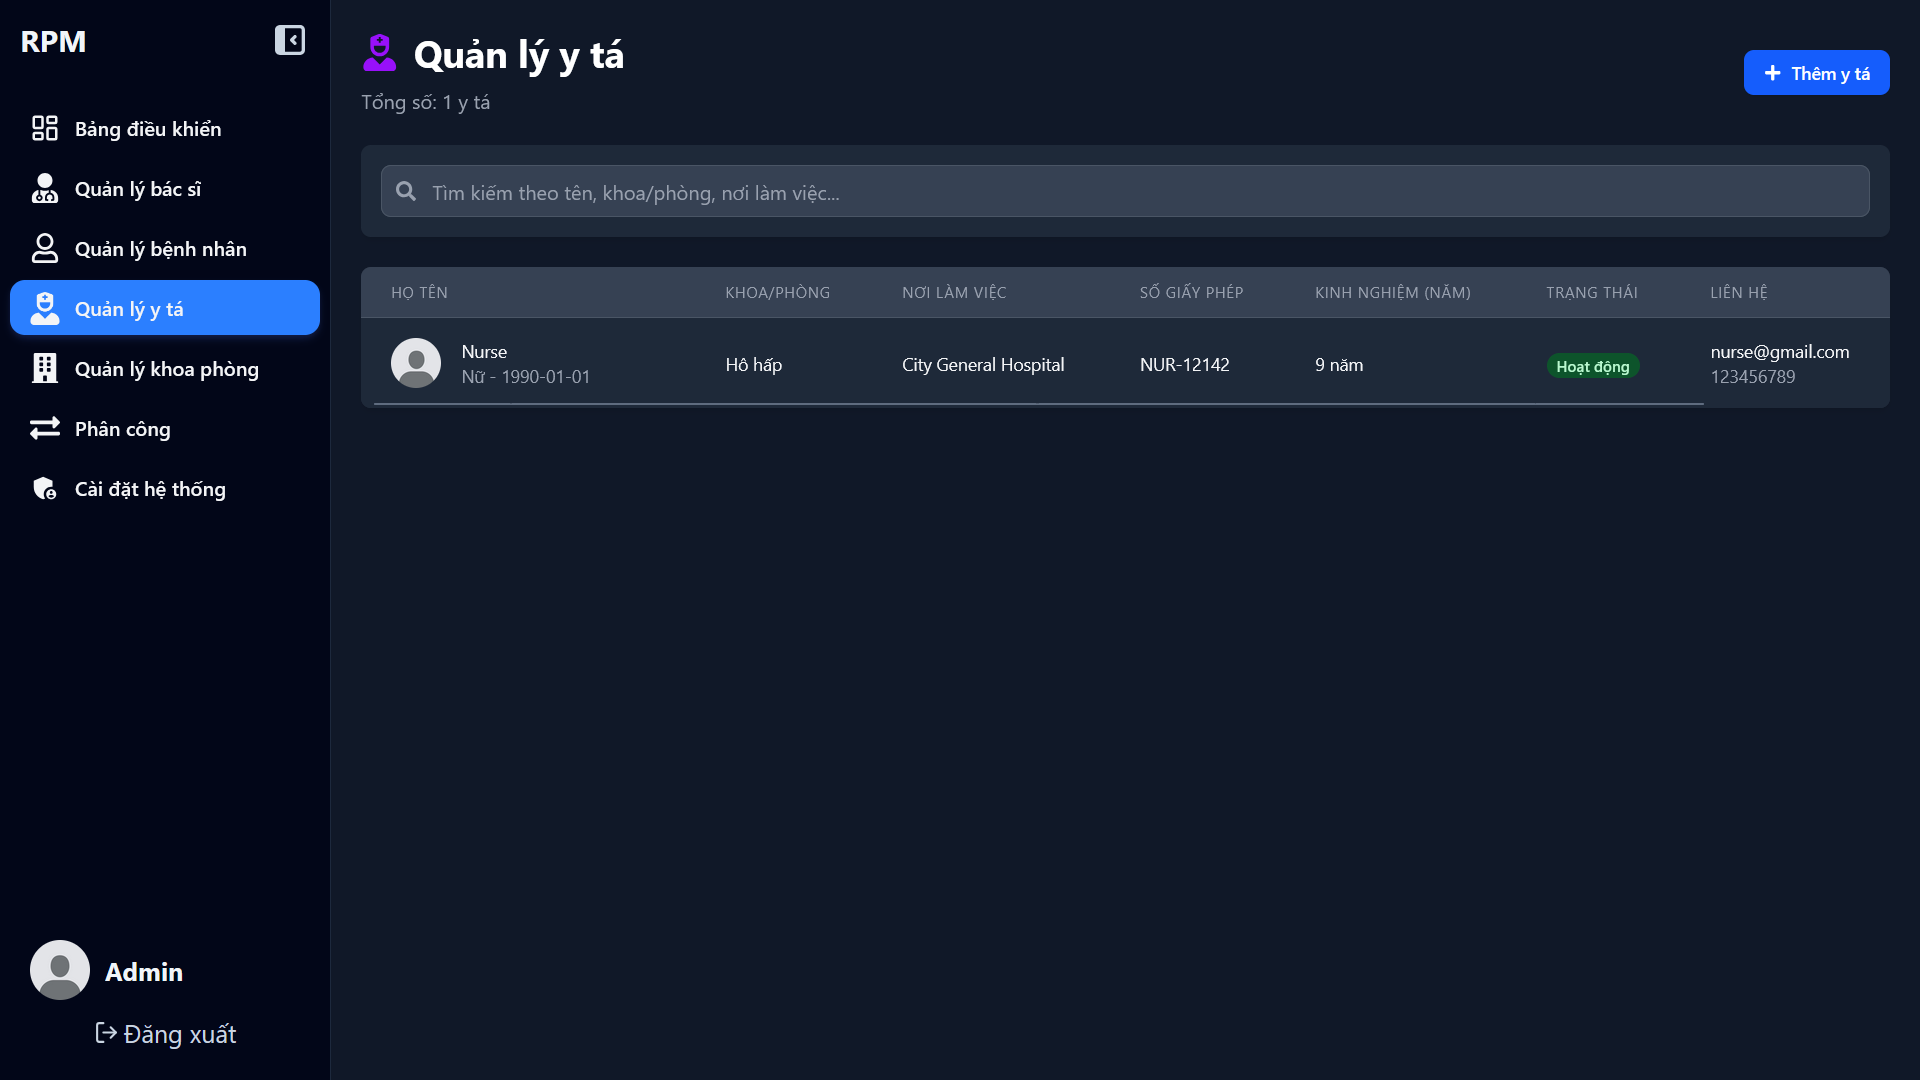
\includegraphics[width=\textwidth,keepaspectratio]{images/Chapter5/Admin/admin-nurse-management.png}
    \end{center}
    \caption{\textit{Màn hình quản lý y tá}}
    \label{chapter5-image26}
    \end{figure}
\end{center}

\subsubsection{Quản lý khoa phòng}
\par Trang quản trị cung cấp chức năng quản lý khoa phòng để tổ chức nhân sự y tế theo các đơn vị chuyên môn. Quản trị viên có thể tạo khoa phòng, cập nhật tên và mô tả, xem danh sách nhân sự trong khoa, thêm thành viên vào khoa hoặc chuyển thành viên giữa các khoa. Chức năng này giúp dữ liệu bác sĩ và y tá có cấu trúc rõ ràng hơn, thay vì chỉ tồn tại dưới dạng danh sách người dùng rời rạc.

\par Đối với hệ thống theo dõi bệnh nhân mãn tính, khoa phòng có thể được sử dụng để phân loại nhân sự theo chuyên môn như tim mạch, nội tiết, chăm sóc mãn tính hoặc các đơn vị điều dưỡng. Mặc dù trong phạm vi đồ án hệ thống chưa triển khai đầy đủ quy trình bệnh viện, việc có module khoa phòng giúp hệ thống có nền tảng để mở rộng sang mô hình vận hành thực tế hơn trong tương lai.

\begin{center}
    \begin{figure}[H]
    \begin{center}
     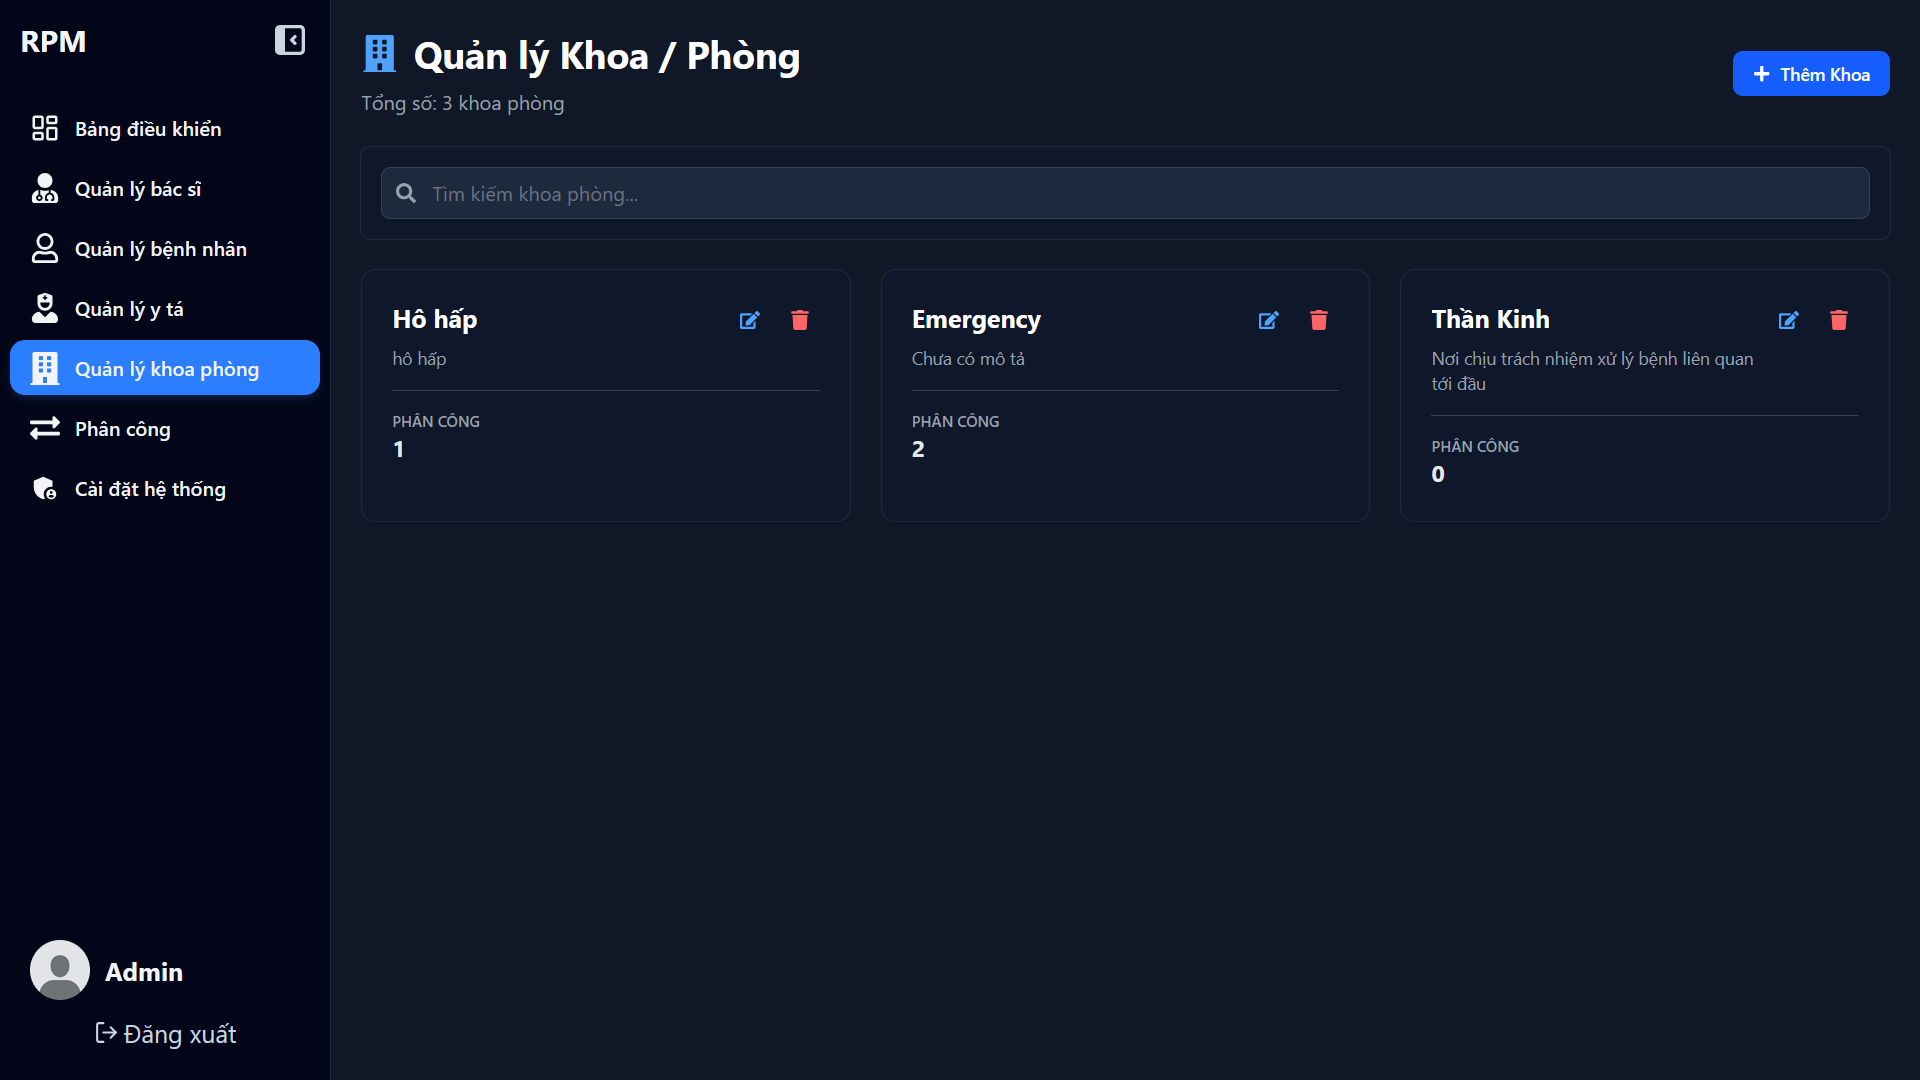
\includegraphics[width=\textwidth,keepaspectratio]{images/Chapter5/Admin/admin-department-management.png}
    \end{center}
    \caption{\textit{Màn hình quản lý khoa phòng}}
    \label{chapter5-image27}
    \end{figure}
\end{center}

\subsubsection{Phân công bệnh nhân}
\par Chức năng phân công cho phép quản trị viên gán bệnh nhân cho bác sĩ phụ trách và y tá theo dõi. Khi phân công, quản trị viên chọn bệnh nhân, chọn bác sĩ và chọn y tá tương ứng. Hệ thống cũng hiển thị danh sách các phân công hiện có, cho phép tìm kiếm, chỉnh sửa hoặc xóa phân công khi cần thiết. Chức năng này là cơ sở để giới hạn phạm vi truy cập dữ liệu theo quan hệ phụ trách.

\par Dữ liệu phân công được sử dụng trong nhiều luồng nghiệp vụ khác nhau. Bác sĩ chỉ xem danh sách bệnh nhân được phân công; y tá chỉ xem danh sách bệnh nhân được giao theo dõi; khi phát sinh cảnh báo, hệ thống có thể xác định bác sĩ phụ trách để tạo tin nhắn hệ thống hoặc cập nhật giao diện bác sĩ. Do đó, phân công không chỉ là chức năng quản trị đơn giản mà còn ảnh hưởng trực tiếp đến tính đúng đắn của luồng theo dõi bệnh nhân.

\begin{center}
    \begin{figure}[H]
    \begin{center}
     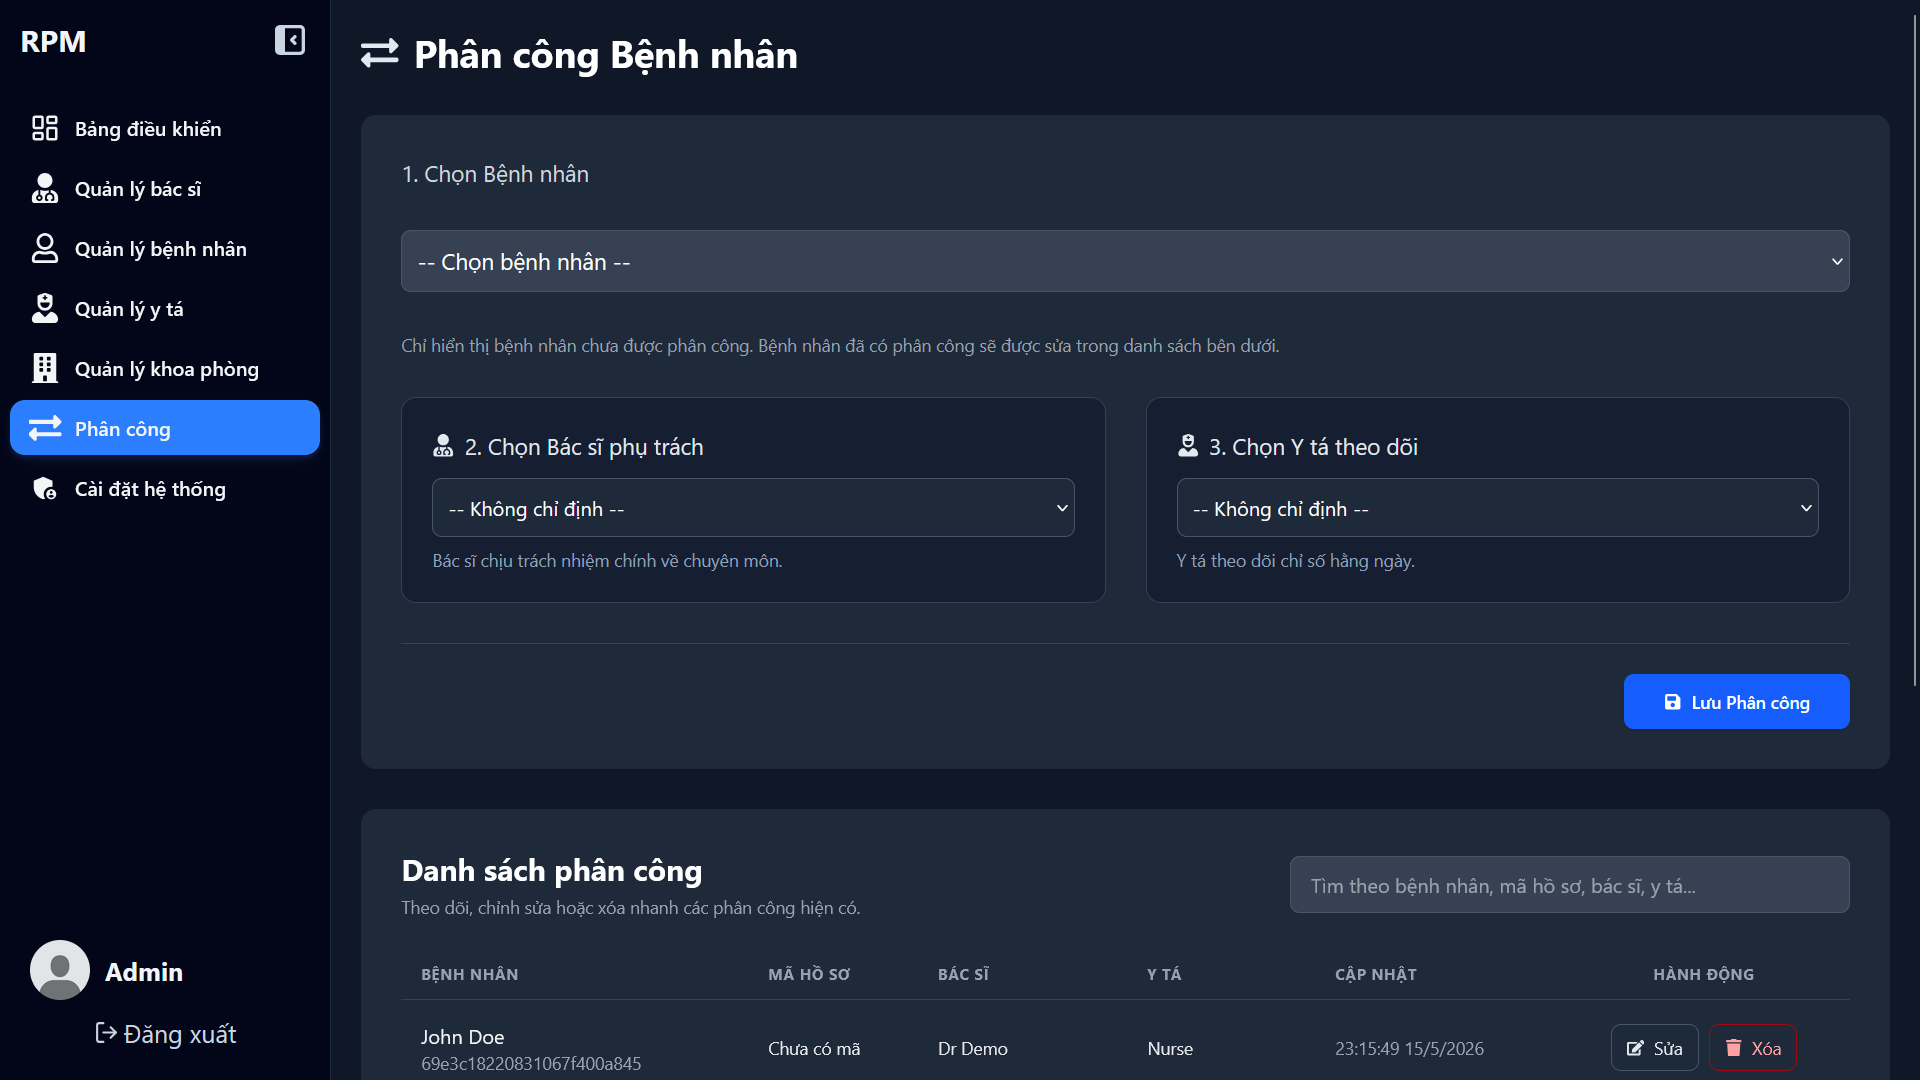
\includegraphics[width=\textwidth,keepaspectratio]{images/Chapter5/Admin/admin-assignment-management.png}
    \end{center}
    \caption{\textit{Màn hình phân công bác sĩ và y tá phụ trách bệnh nhân}}
    \label{chapter5-image28}
    \end{figure}
\end{center}

\subsubsection{Lịch sử hoạt động}
\par Chức năng lịch sử hoạt động giúp quản trị viên theo dõi các thao tác đã diễn ra trong hệ thống. Mỗi bản ghi hoạt động có thể bao gồm loại hoạt động, người thực hiện, hành động, thời gian, tài nguyên bị tác động và các thông tin liên quan. Quản trị viên có thể lọc theo ngày hoặc loại hoạt động để kiểm tra các sự kiện quan trọng.

\par Trong một hệ thống xử lý dữ liệu sức khỏe, việc ghi nhận lịch sử hoạt động có ý nghĩa quan trọng đối với vận hành và kiểm tra sự cố. Khi có thay đổi bất thường trong dữ liệu người dùng, phân công hoặc trạng thái tài khoản, quản trị viên có thể xem lại lịch sử để xác định thao tác được thực hiện khi nào và bởi ai. Mặc dù trong phạm vi đồ án chức năng này chưa phải một hệ thống audit log hoàn chỉnh theo chuẩn y tế, nó vẫn là nền tảng cần thiết cho việc quản trị hệ thống.

\begin{center}
    \begin{figure}[H]
    \begin{center}
     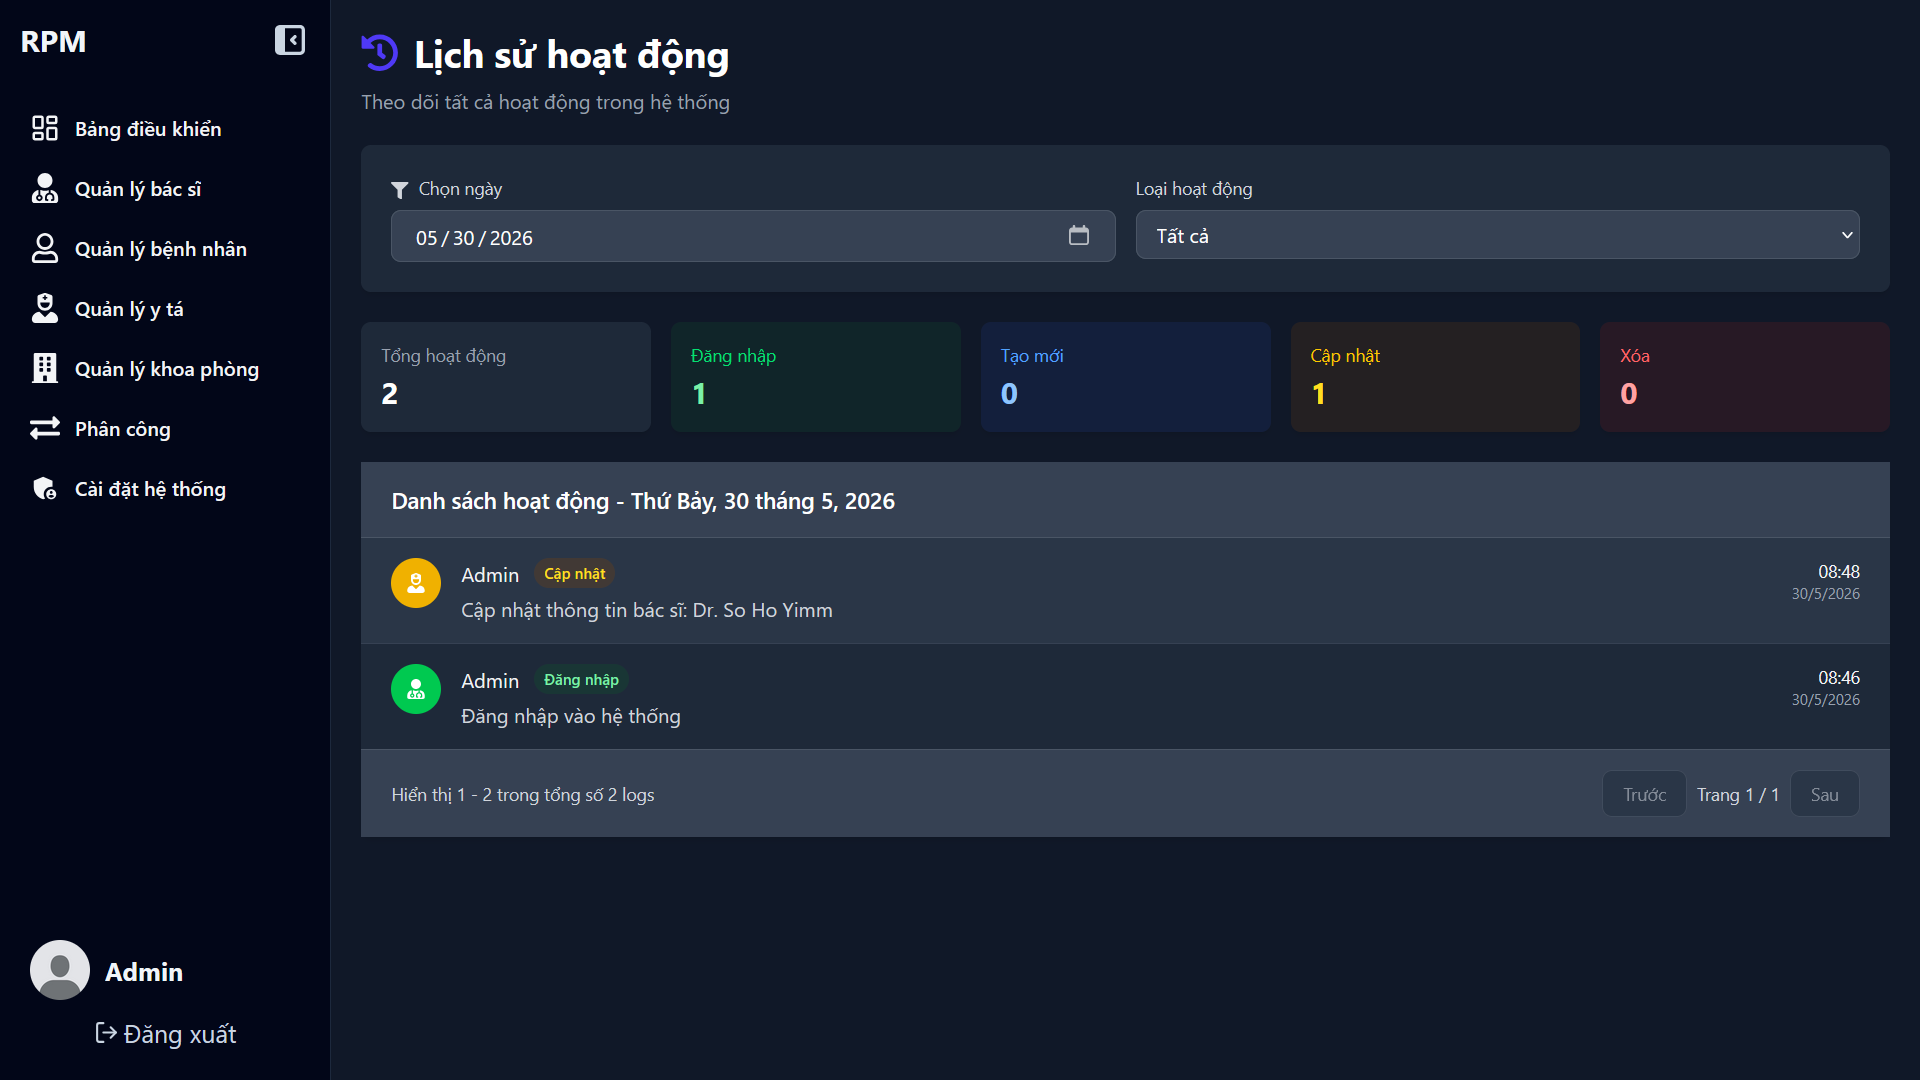
\includegraphics[width=\textwidth,keepaspectratio]{images/Chapter5/Admin/admin-activity-history.png}
    \end{center}
    \caption{\textit{Màn hình lịch sử hoạt động của hệ thống}}
    \label{chapter5-image29}
    \end{figure}
\end{center}

\subsubsection{Cài đặt hệ thống}
\par Trang quản trị cũng cung cấp màn hình cài đặt hệ thống và giao diện. Quản trị viên có thể điều chỉnh một số thiết lập hiển thị như theme sáng/tối, kiểu chữ và kích thước chữ. Các tùy chỉnh này giúp giao diện quản trị dễ sử dụng hơn trong nhiều môi trường làm việc khác nhau.

\par Mặc dù chức năng cài đặt trong phiên bản hiện tại chủ yếu tập trung vào trải nghiệm giao diện, đây vẫn là một phần cần thiết của trang quản trị. Trong tương lai, màn hình này có thể được mở rộng để cấu hình các thông số vận hành khác như chính sách thông báo, thiết lập bảo mật, cấu hình thời gian nhắc nhở mặc định hoặc các thông số hệ thống khác.

\begin{center}
    \begin{figure}[H]
    \begin{center}
     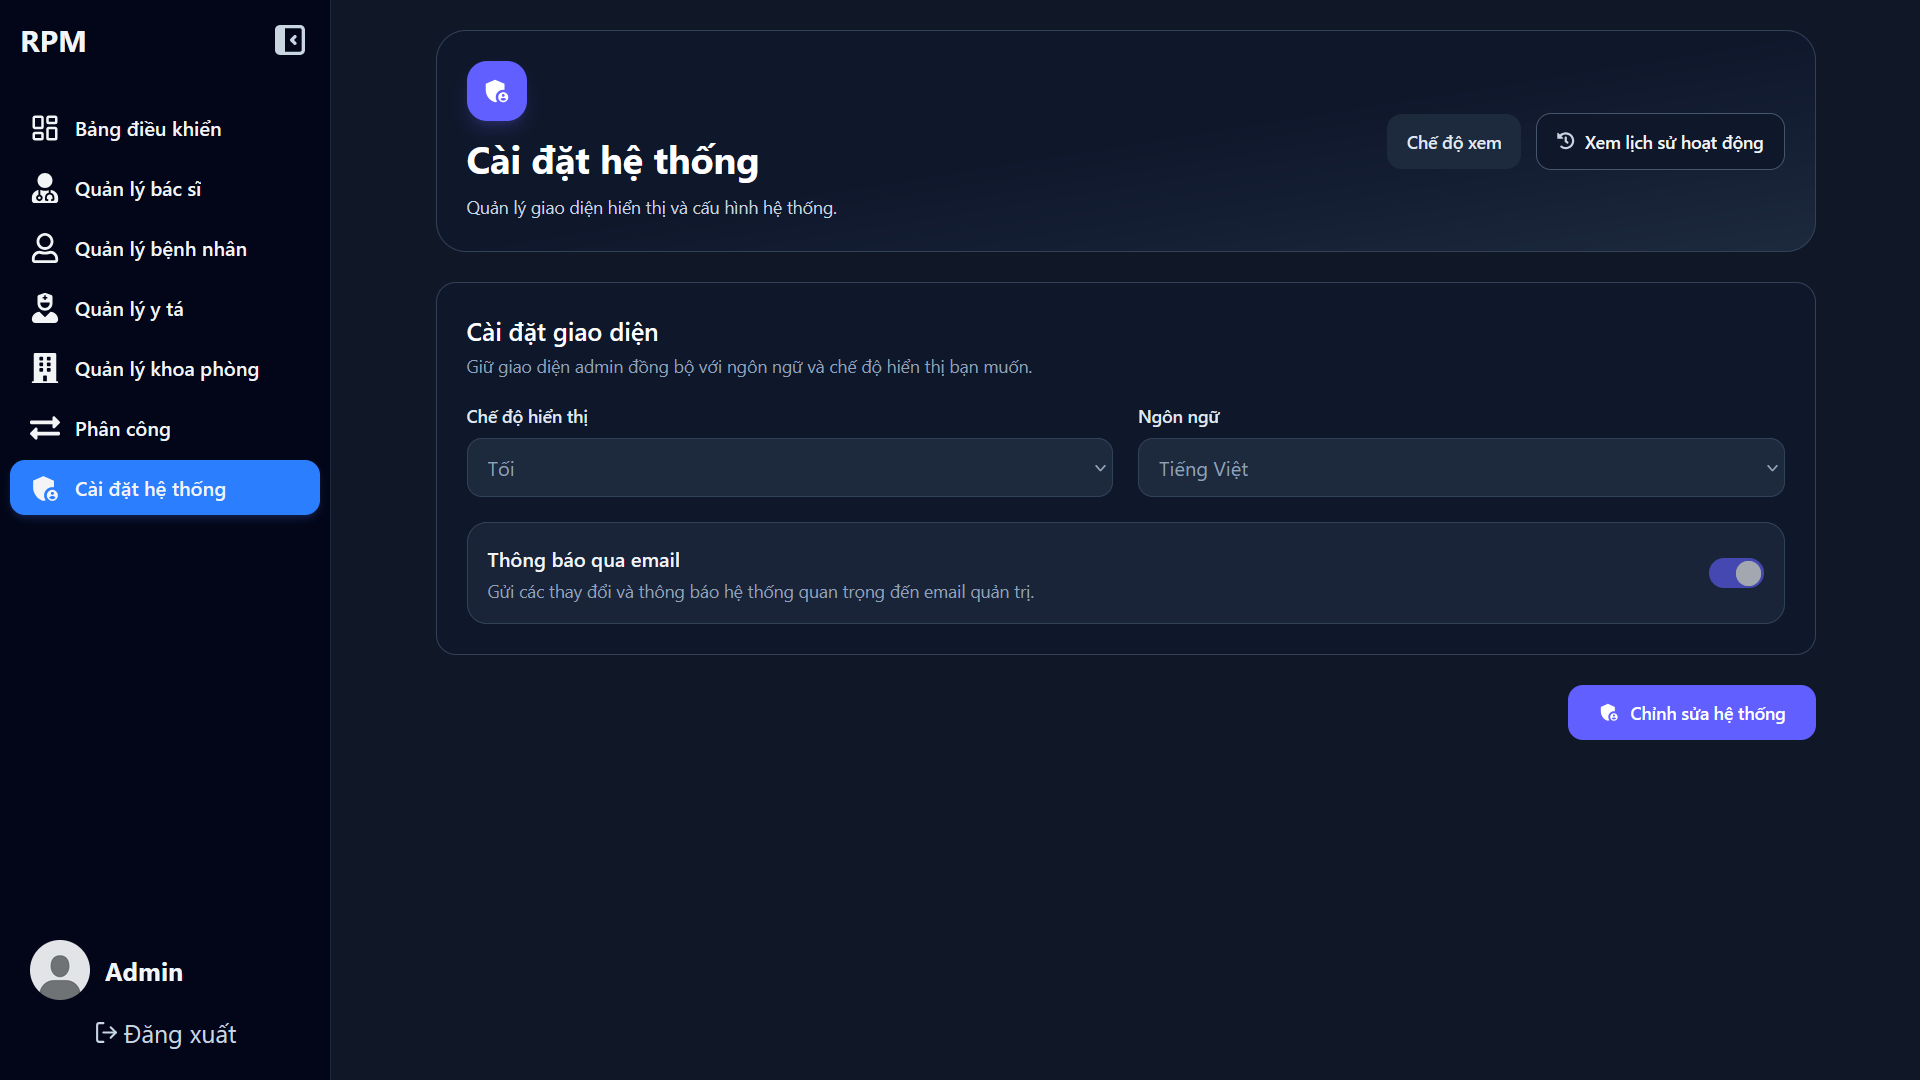
\includegraphics[width=\textwidth,keepaspectratio]{images/Chapter5/Admin/admin-system-settings.png}
    \end{center}
    \caption{\textit{Màn hình cài đặt hệ thống trên trang quản trị}}
    \label{chapter5-image30}
    \end{figure}
\end{center}

\newpage
\subsection{Hệ thống backend và API}

\par Backend là thành phần trung tâm của hệ thống, chịu trách nhiệm xử lý nghiệp vụ, xác thực người dùng, phân quyền theo vai trò, lưu trữ dữ liệu, sinh cảnh báo, gửi thông báo, quản lý workflow nền và cung cấp API cho các ứng dụng client. Backend được xây dựng bằng Go với Gin framework, sử dụng MongoDB làm cơ sở dữ liệu chính, Redis cho các nhu cầu thời gian thực và Temporal cho các workflow xử lý nền. Nhờ có backend, các thành phần mobile, web bác sĩ và admin web có thể hoạt động nhất quán trên cùng một nguồn dữ liệu.

\subsubsection{Tài liệu API bằng Swagger}
\par Hệ thống backend cung cấp tài liệu API thông qua Swagger UI. Đây là công cụ hỗ trợ nhóm phát triển kiểm tra endpoint, xem cấu trúc request/response và thử gọi API trong quá trình phát triển. Tài liệu API giúp quá trình phối hợp giữa backend, frontend và mobile thuận tiện hơn vì các thành viên có thể tra cứu nhanh endpoint cần dùng thay vì phải hỏi trực tiếp hoặc đọc mã nguồn backend.

\par Các nhóm API chính bao gồm xác thực, người dùng, bệnh nhân, bác sĩ, y tá, khoa phòng, phân công, dữ liệu đo, ngưỡng, cảnh báo, nhắc nhở, chat, thông báo, realtime và lịch sử hoạt động. Việc gom các endpoint theo nhóm nghiệp vụ giúp tài liệu API dễ theo dõi hơn và hỗ trợ quá trình kiểm thử thủ công trong giai đoạn hoàn thiện sản phẩm.

\begin{center}
    \begin{figure}[H]
    \begin{center}
     \includegraphics[width=\textwidth,keepaspectratio]{images/Chapter5/Backend/backend-swagger.png}
    \end{center}
    \caption{\textit{Giao diện tài liệu API bằng Swagger}}
    \label{chapter5-image31}
    \end{figure}
\end{center}

\subsubsection{Xác thực, phân quyền và quản lý phiên}
\par Backend hỗ trợ các chức năng xác thực như đăng ký, đăng nhập, lấy thông tin người dùng hiện tại, làm mới phiên đăng nhập, đăng xuất, đặt lại mật khẩu, kích hoạt tài khoản và đăng nhập Google OAuth2. Sau khi đăng nhập, hệ thống sử dụng token để xác thực các request tiếp theo. Các API quan trọng được bảo vệ bằng middleware JWT và middleware kiểm tra vai trò.

\par Hệ thống có các vai trò chính gồm bệnh nhân, bác sĩ, y tá và quản trị viên. Mỗi vai trò chỉ được truy cập các chức năng phù hợp với nhiệm vụ của mình. Ví dụ, bác sĩ có quyền cấu hình ngưỡng và quản lý nhắc nhở cho bệnh nhân; bệnh nhân có quyền xem cảnh báo và thông báo của chính mình; y tá có quyền xem bệnh nhân được phân công và nhập liệu hỗ trợ; quản trị viên có quyền quản lý người dùng, khoa phòng, phân công và lịch sử hoạt động. Cơ chế phân quyền này là nền tảng quan trọng để bảo vệ dữ liệu sức khỏe trong hệ thống.

\subsubsection{Lưu trữ dữ liệu đo sức khỏe}
\par Backend cung cấp API để tạo, cập nhật và truy vấn dữ liệu đo sức khỏe. Mỗi bản đo có thể chứa các chỉ số như huyết áp tâm thu, huyết áp tâm trương, MAP, đường huyết, thân nhiệt, nhịp tim, nhịp thở, SpO2, thời điểm đo và ghi chú. Dữ liệu sau khi được gửi lên backend sẽ được lưu vào MongoDB và có thể được truy vấn lại bởi ứng dụng di động hoặc web bác sĩ.

\par Sau khi lưu dữ liệu đo, backend kích hoạt workflow xử lý cảnh báo để đánh giá chỉ số vừa nhập với ngưỡng an toàn tương ứng. Cách tổ chức này giúp luồng nhập liệu không chỉ dừng lại ở việc lưu dữ liệu, mà còn tạo ra phản hồi tự động khi phát hiện chỉ số bất thường. Đây là phần nghiệp vụ quan trọng nhất của hệ thống RPM.

\subsubsection{Workflow cảnh báo tự động}
\par Hệ thống sử dụng Temporal để xử lý workflow cảnh báo. Khi một bản đo mới được tạo, backend khởi động workflow đánh giá dữ liệu đo. Workflow sẽ lấy thông tin bản đo, lấy bộ ngưỡng mới nhất của bệnh nhân, so sánh từng chỉ số với ngưỡng tương ứng và tạo cảnh báo nếu phát hiện vi phạm. Cảnh báo sau đó được lưu vào cơ sở dữ liệu và có thể được hiển thị ở phía bệnh nhân, bác sĩ hoặc y tá tùy theo vai trò.

\par Ngoài việc lưu cảnh báo, workflow còn có thể tạo thông báo, gửi push notification và tạo tin nhắn hệ thống trong cuộc trò chuyện giữa bệnh nhân với bác sĩ. Nhờ đó, một sự kiện bất thường có thể được lan truyền đến các thành phần liên quan của hệ thống mà không cần người dùng thực hiện nhiều thao tác thủ công. Cơ chế này giúp hệ thống có tính chủ động hơn trong quá trình theo dõi bệnh nhân từ xa.

\begin{center}
    \begin{figure}[H]
    \begin{center}
     \includegraphics[width=\textwidth,keepaspectratio]{images/Chapter5/Backend/backend-alert-workflow-result.png}
    \end{center}
    \caption{\textit{Kết quả xử lý workflow cảnh báo tự động}}
    \label{chapter5-image32}
    \end{figure}
\end{center}

\subsubsection{Workflow nhắc nhở}
\par Backend cũng sử dụng Temporal để xử lý nhắc nhở định kỳ. Khi bác sĩ tạo một nhắc nhở cho bệnh nhân, backend lưu nhắc nhở vào cơ sở dữ liệu và khởi động workflow tương ứng. Workflow sẽ tính thời điểm gửi tiếp theo dựa trên giờ, phút, ngày trong tuần, ngày bắt đầu, ngày kết thúc và trạng thái của nhắc nhở. Khi đến thời điểm phù hợp, workflow gửi thông báo cho bệnh nhân và tiếp tục tính lần gửi kế tiếp nếu nhắc nhở còn hiệu lực.

\par Cách xử lý bằng workflow giúp chức năng nhắc nhở ổn định và dễ mở rộng hơn so với việc xử lý hoàn toàn trong request HTTP. Trong tương lai, workflow nhắc nhở có thể được mở rộng để hỗ trợ nhiều loại nhắc nhở hơn, ví dụ nhắc tái khám, nhắc uống thuốc theo toa, nhắc đo lại sau khi có cảnh báo hoặc nhắc xác nhận đã thực hiện một hành động chăm sóc.

\begin{center}
    \begin{figure}[H]
    \begin{center}
     \includegraphics[width=\textwidth,keepaspectratio]{images/Chapter5/Backend/backend-reminder-workflow-result.png}
    \end{center}
    \caption{\textit{Kết quả xử lý workflow nhắc nhở cho bệnh nhân}}
    \label{chapter5-image33}
    \end{figure}
\end{center}

\subsubsection{Thông báo đẩy và cập nhật thời gian thực}
\par Backend tích hợp Firebase Cloud Messaging để gửi push notification đến thiết bị di động. Khi ứng dụng di động lấy được token thiết bị, token được gửi về backend và lưu lại. Khi có cảnh báo hoặc nhắc nhở, backend sử dụng token còn hoạt động để gửi thông báo đến thiết bị của bệnh nhân. Ngoài push notification, backend cũng lưu thông báo vào collection riêng để người dùng có thể xem lại trong ứng dụng.

\par Đối với cập nhật thời gian thực, hệ thống sử dụng WebSocket cho chức năng chat và realtime notification. Redis Pub/Sub được dùng để phát sự kiện nội bộ, giúp các handler WebSocket có thể gửi sự kiện đến client đang kết nối. Nhờ đó, bác sĩ có thể nhận được tin nhắn hoặc sự kiện cảnh báo mới mà không cần liên tục tải lại trang. Đây là một kết quả quan trọng vì hệ thống theo dõi từ xa cần phản hồi nhanh khi có dữ liệu bất thường.

\subsection{Triển khai sản phẩm lên AWS}

\par Ngoài việc chạy được ở môi trường local, hệ thống đã được cấu hình để triển khai lên AWS phục vụ kiểm thử và demo. Nhóm triển khai frontend và backend theo hướng tách biệt. Các ứng dụng web được build thành static files, lưu trữ trên Amazon S3 và phục vụ người dùng qua Cloudflare để thiết lập HTTPS, trong khi backend được đóng gói bằng Docker và chạy trên Amazon EC2. Cách triển khai này phù hợp với quy mô đồ án vì dễ kiểm soát, dễ cập nhật và đủ linh hoạt để mở rộng trong tương lai.

\subsubsection{Triển khai web bác sĩ và admin web lên Amazon S3}
\par Ứng dụng web dành cho bác sĩ và trang quản trị được build bằng Vite. Sau khi build, thư mục kết quả được đồng bộ lên các bucket Amazon S3 tương ứng thông qua GitHub Actions. Người dùng truy cập giao diện web qua tên miền được cấu hình trên Cloudflare, trong khi các request nghiệp vụ được gửi đến backend thông qua API URL được cấu hình trong biến môi trường production.

\par Việc triển khai static web trên S3 giúp frontend không phụ thuộc vào máy chủ backend để phục vụ file giao diện. Backend chỉ cần tập trung xử lý API, còn S3 chịu trách nhiệm lưu trữ các file HTML, CSS, JavaScript và assets. Cloudflare được đặt phía trước S3 để cung cấp HTTPS, quản lý tên miền và chuyển tiếp request từ người dùng đến bucket tương ứng. Cách kết hợp S3 và Cloudflare giúp frontend có thể truy cập an toàn qua HTTPS mà không cần tự vận hành máy chủ web riêng cho giao diện.

\begin{center}
    \begin{figure}[H]
    \begin{center}
     \includegraphics[width=\textwidth,keepaspectratio]{images/Chapter5/Deployment/aws-s3-frontend-deployment.png}
    \end{center}
    \caption{\textit{Ứng dụng web bác sĩ và admin web được triển khai lên Amazon S3}}
    \label{chapter5-image34}
    \end{figure}
\end{center}

\subsubsection{Triển khai backend trên Amazon EC2 bằng Docker}
\par Backend được triển khai trên Amazon EC2 bằng Docker Compose. Trên máy chủ EC2, các service chính bao gồm API server, Temporal server, Temporal worker, Redis và Nginx reverse proxy. Nginx tiếp nhận request từ internet, xử lý proxy và chuyển tiếp request đến API server nội bộ. Đối với các kết nối WebSocket, Nginx cũng được cấu hình để hỗ trợ nâng cấp kết nối.

\par Việc sử dụng Docker giúp môi trường triển khai nhất quán hơn với môi trường phát triển. Khi có phiên bản mới của backend, nhóm có thể build Docker image, push image lên registry và cập nhật container trên EC2. Cách triển khai này giảm rủi ro do khác biệt môi trường, đồng thời giúp nhóm dễ kiểm tra log, khởi động lại service và quản lý các thành phần backend trên cùng một máy chủ.

\begin{center}
    \begin{figure}[H]
    \begin{center}
     \includegraphics[width=\textwidth,keepaspectratio]{images/Chapter5/Deployment/aws-ec2-backend-deployment.png}
    \end{center}
    \caption{\textit{Backend được triển khai trên Amazon EC2 bằng Docker Compose}}
    \label{chapter5-image35}
    \end{figure}
\end{center}

\subsubsection{CI/CD với GitHub Actions}
\par Nhóm đã thiết lập GitHub Actions để hỗ trợ tự động hóa quá trình build và triển khai. Đối với frontend web và admin web, workflow thực hiện các bước như checkout mã nguồn, cài đặt Node.js, cài đặt dependencies, tạo file môi trường production, build ứng dụng và đồng bộ thư mục build lên Amazon S3. Đối với backend, workflow thực hiện các bước kiểm tra mã nguồn, chạy test, build Docker image, push image và cập nhật hệ thống trên EC2.

\par Việc áp dụng CI/CD giúp giảm thao tác thủ công khi triển khai. Mỗi khi mã nguồn được cập nhật vào nhánh triển khai, hệ thống có thể tự động thực hiện các bước cần thiết để đưa phiên bản mới lên môi trường kiểm thử hoặc demo. Điều này đặc biệt hữu ích với một hệ thống có nhiều thành phần như RPM, vì nếu triển khai thủ công toàn bộ frontend, backend, Nginx, Docker và biến môi trường thì rất dễ xảy ra thiếu sót.

\begin{center}
    \begin{figure}[H]
    \begin{center}
     \includegraphics[width=\textwidth,keepaspectratio]{images/Chapter5/Deployment/github-actions-cicd.png}
    \end{center}
    \caption{\textit{Quy trình CI/CD bằng GitHub Actions}}
    \label{chapter5-image36}
    \end{figure}
\end{center}

\subsubsection{Kiểm thử truy cập qua internet}
\par Sau khi triển khai, nhóm tiến hành kiểm thử các luồng chính thông qua môi trường internet thay vì chỉ chạy local. Các luồng được kiểm tra bao gồm đăng nhập web bác sĩ, đăng nhập admin, truy cập dashboard, gọi API lấy danh sách bệnh nhân, nhập chỉ số trên mobile, xem cảnh báo, tạo nhắc nhở, gửi tin nhắn và kiểm tra WebSocket. Việc kiểm thử trên môi trường triển khai giúp phát hiện các lỗi thường không xuất hiện ở local như sai biến môi trường, CORS, cấu hình reverse proxy, security group, lỗi WebSocket hoặc sai đường dẫn API.

\par Kết quả triển khai thử nghiệm cho thấy hệ thống có thể vận hành theo mô hình nhiều thành phần trên AWS. Mặc dù cấu hình hiện tại phù hợp hơn cho demo và thử nghiệm đồ án, nó đã cung cấp nền tảng để nhóm hiểu và chứng minh khả năng đưa sản phẩm từ môi trường phát triển lên môi trường triển khai thực tế. Trong tương lai, hệ thống có thể được mở rộng bằng cách tách worker ra nhiều instance, bổ sung giám sát vận hành hoặc chuyển sang các dịch vụ container chuyên dụng hơn như ECS nếu quy mô người dùng tăng.

\begin{center}
    \begin{figure}[H]
    \begin{center}
     \includegraphics[width=\textwidth,keepaspectratio]{images/Chapter5/Deployment/deployed-system-overview.png}
    \end{center}
    \caption{\textit{Kiểm thử hệ thống sau khi triển khai trên AWS}}
    \label{chapter5-image37}
    \end{figure}
\end{center}

\newpage
\section{Kết quả chức năng đạt được}

\par Dựa trên phạm vi đã đặt ra, hệ thống đã hoàn thành phần lớn các chức năng cốt lõi cần có của một mô hình theo dõi bệnh nhân từ xa ở mức Proof-of-Concept. Các chức năng này được chia theo từng vai trò người dùng và từng thành phần hệ thống. Bảng dưới đây tổng hợp các nhóm chức năng chính đã đạt được.

\begin{center}
\begin{longtable}{|p{3.2cm}|p{5cm}|p{6.2cm}|}
    \hline
    \textbf{Thành phần} & \textbf{Chức năng đã hoàn thành} & \textbf{Ý nghĩa trong hệ thống} \\
    \hline
    \endfirsthead
    \hline
    \textbf{Thành phần} & \textbf{Chức năng đã hoàn thành} & \textbf{Ý nghĩa trong hệ thống} \\
    \hline
    \endhead

    Ứng dụng di động bệnh nhân &
    Đăng nhập, đăng ký, nhập chỉ số, xem lịch sử đo, theo dõi cảnh báo, nhận thông báo, chat với bác sĩ, xem hồ sơ cá nhân. &
    Giúp bệnh nhân chủ động ghi nhận và theo dõi sức khỏe hằng ngày, đồng thời có kênh trao đổi với bác sĩ khi cần tư vấn. \\
    \hline

    Ứng dụng di động y tá &
    Xem danh sách bệnh nhân được phân công, tìm kiếm bệnh nhân, nhập chỉ số cho bệnh nhân, xem hồ sơ y tá. &
    Hỗ trợ nhân viên y tế tham gia vào quá trình theo dõi và nhập liệu, phù hợp với bối cảnh bệnh nhân cần được hỗ trợ. \\
    \hline

    Web bác sĩ &
    Dashboard, danh sách bệnh nhân, chi tiết bệnh nhân, biểu đồ xu hướng, lịch sử đo, cấu hình ngưỡng, cảnh báo, nhắc nhở, chat, xuất báo cáo. &
    Giúp bác sĩ theo dõi bệnh nhân từ xa, phát hiện chỉ số bất thường và quản lý kế hoạch theo dõi cho từng bệnh nhân. \\
    \hline

    Admin web &
    Dashboard quản trị, quản lý bác sĩ, bệnh nhân, y tá, khoa phòng, phân công, lịch sử hoạt động và cài đặt hệ thống. &
    Hỗ trợ quản trị viên vận hành hệ thống, tổ chức dữ liệu người dùng và kiểm soát quan hệ phân công giữa bệnh nhân với nhân viên y tế. \\
    \hline

    Backend &
    RESTful API, xác thực JWT, phân quyền vai trò, MongoDB, workflow cảnh báo, workflow nhắc nhở, WebSocket, Redis Pub/Sub, FCM, Swagger. &
    Đóng vai trò trung tâm xử lý nghiệp vụ, lưu trữ dữ liệu, sinh cảnh báo, gửi thông báo và đồng bộ dữ liệu giữa các client. \\
    \hline

    Triển khai &
    Frontend lưu trữ trên Amazon S3 và phục vụ qua Cloudflare để thiết lập HTTPS, backend triển khai trên Amazon EC2 bằng Docker Compose, CI/CD bằng GitHub Actions. &
    Chứng minh hệ thống có thể vận hành ngoài môi trường local và phục vụ kiểm thử, demo thông qua internet. \\
    \hline

    \caption{Tổng hợp kết quả chức năng đạt được của hệ thống}
    \label{chapter5-table01}
\end{longtable}
\end{center}

\section{Số liệu triển khai thử nghiệm}

\par Trong phạm vi đồ án, hệ thống được triển khai chủ yếu nhằm phục vụ kiểm thử và demo chức năng. Nhóm chưa tiến hành triển khai thực nghiệm với số lượng lớn người dùng thật tại cơ sở y tế, vì vậy các số liệu như số bệnh nhân thực tế, số bác sĩ sử dụng thật, số lượt đo hằng ngày hoặc số cảnh báo phát sinh trong môi trường lâm sàng chưa được xem là dữ liệu đánh giá chính thức. Thay vào đó, nhóm sử dụng dữ liệu kiểm thử và tài khoản mẫu để kiểm tra các luồng nghiệp vụ chính.

\par Các tiêu chí kiểm thử tập trung vào việc đảm bảo hệ thống có thể vận hành xuyên suốt theo từng vai trò. Với bệnh nhân, nhóm kiểm tra luồng đăng nhập, nhập chỉ số, xem lịch sử, nhận cảnh báo, xem thông báo và nhắn tin với bác sĩ. Với bác sĩ, nhóm kiểm tra luồng xem danh sách bệnh nhân, xem biểu đồ, cấu hình ngưỡng, nhận cảnh báo, xác nhận cảnh báo, tạo nhắc nhở và gửi tin nhắn. Với y tá, nhóm kiểm tra luồng xem danh sách bệnh nhân được phân công và nhập chỉ số hỗ trợ. Với quản trị viên, nhóm kiểm tra luồng quản lý tài khoản, khoa phòng, phân công và lịch sử hoạt động.

\par Kết quả kiểm thử thử nghiệm cho thấy hệ thống đã đáp ứng được các luồng sử dụng chính ở mức đồ án. Các thành phần frontend, mobile, backend và hạ tầng deploy có thể phối hợp với nhau trong những kịch bản cơ bản. Tuy nhiên, để đánh giá chính xác hiệu quả trong môi trường thực tế, hệ thống vẫn cần được triển khai với dữ liệu thật, người dùng thật và quy trình vận hành của một đơn vị y tế cụ thể trong các giai đoạn phát triển sau.

\begin{center}
    \begin{figure}[H]
    \begin{center}
     \includegraphics[width=\textwidth,keepaspectratio]{images/Chapter5/Statistics/testing-summary.png}
    \end{center}
    \caption{\textit{Tổng hợp kết quả kiểm thử thử nghiệm các luồng chính của hệ thống}}
    \label{chapter5-image38}
    \end{figure}
\end{center}

\section{Đánh giá kết quả đạt được}

\par Nhìn chung, hệ thống đã đạt được mục tiêu xây dựng một mô hình thử nghiệm cho bài toán theo dõi bệnh nhân từ xa. Các chức năng chính của đề tài như nhập dữ liệu sức khỏe, lưu trữ dữ liệu, hiển thị lịch sử đo, hiển thị biểu đồ xu hướng, cấu hình ngưỡng, sinh cảnh báo tự động, gửi thông báo, tạo nhắc nhở và trao đổi giữa bệnh nhân với bác sĩ đều đã được xây dựng ở mức có thể sử dụng và demo. Việc bổ sung vai trò y tá và quản trị viên cũng giúp hệ thống có tính hoàn chỉnh hơn so với phạm vi tối thiểu ban đầu.

\par Về mặt kỹ thuật, nhóm đã xây dựng được hệ thống nhiều thành phần với mobile, web, admin, backend, MongoDB, Redis, Temporal, FCM, WebSocket, Docker và AWS. Các công nghệ này giúp sản phẩm không chỉ dừng lại ở giao diện tĩnh mà có luồng xử lý nghiệp vụ đầy đủ từ nhập liệu đến cảnh báo và thông báo. Việc triển khai lên AWS cũng cho thấy nhóm có khả năng đưa hệ thống ra khỏi môi trường local, cấu hình hạ tầng và kiểm thử trên môi trường gần với thực tế hơn.

\par Về mặt sử dụng, hệ thống đã cung cấp giao diện riêng cho từng nhóm người dùng. Bệnh nhân sử dụng ứng dụng di động với các thao tác đơn giản; bác sĩ sử dụng web dashboard để xem dữ liệu và quản lý cảnh báo; y tá sử dụng mobile để theo dõi và nhập liệu hỗ trợ; quản trị viên sử dụng admin web để quản lý dữ liệu vận hành. Cách phân chia này giúp mỗi vai trò chỉ tập trung vào các chức năng phù hợp với nhiệm vụ của mình, góp phần giảm sự phức tạp trong trải nghiệm sử dụng.

\section{Một số hạn chế còn tồn tại}

\par Bên cạnh các kết quả đã đạt được, hệ thống vẫn còn một số hạn chế cần được ghi nhận. Thứ nhất, dữ liệu sức khỏe trong phiên bản hiện tại vẫn được nhập thủ công bởi bệnh nhân hoặc y tá, chưa tích hợp trực tiếp với các thiết bị đo như máy đo huyết áp, máy đo đường huyết hoặc thiết bị đeo. Điều này giúp hệ thống dễ triển khai trong phạm vi đồ án, nhưng dữ liệu có thể bị ảnh hưởng bởi sai sót nhập liệu, quên nhập hoặc nhập không đúng thời điểm đo.

\par Thứ hai, cơ chế cảnh báo hiện tại dựa trên ngưỡng an toàn do bác sĩ cấu hình hoặc ngưỡng cố định trong hệ thống. Cách tiếp cận này có ưu điểm là đơn giản, dễ hiểu và dễ kiểm soát, nhưng chưa thể phản ánh đầy đủ bối cảnh lâm sàng phức tạp của từng bệnh nhân. Trong thực tế, việc đánh giá một chỉ số bất thường có thể phụ thuộc vào tuổi, bệnh nền, thuốc đang sử dụng, triệu chứng đi kèm và nhiều yếu tố khác. Do đó, cảnh báo của hệ thống chỉ nên được xem là công cụ hỗ trợ theo dõi, không phải kết luận chẩn đoán.

\par Thứ ba, hệ thống chưa được kiểm thử với quy mô lớn và chưa có dữ liệu thực nghiệm từ môi trường y tế thật. Các kết quả hiện tại chủ yếu dựa trên môi trường thử nghiệm, tài khoản mẫu và dữ liệu mẫu. Nếu triển khai thực tế, hệ thống cần được kiểm thử thêm về hiệu năng, bảo mật, tính ổn định, khả năng chịu tải, quy trình vận hành và sự phù hợp với nhu cầu của bác sĩ, y tá và bệnh nhân trong điều kiện sử dụng thật.

\par Cuối cùng, hạ tầng triển khai hiện tại phù hợp với mục tiêu demo và kiểm thử đồ án, nhưng vẫn cần được mở rộng nếu vận hành ở quy mô lớn. Một máy chủ EC2 chạy nhiều service bằng Docker Compose giúp triển khai đơn giản, nhưng trong tương lai có thể cần tách các thành phần quan trọng, bổ sung giám sát hệ thống, sao lưu dữ liệu, tự động khôi phục, bảo mật secrets, CDN cho frontend và các cơ chế kiểm soát truy cập chặt chẽ hơn.

\section{Định hướng hoàn thiện sau đồ án}

\par Từ những kết quả và hạn chế đã ghi nhận, nhóm đề xuất một số định hướng phát triển tiếp theo cho hệ thống. Trước hết, hệ thống có thể được mở rộng để tích hợp trực tiếp với các thiết bị đo sức khỏe tại nhà. Khi dữ liệu được đồng bộ tự động từ thiết bị, hệ thống có thể giảm sai sót nhập liệu và tăng tần suất theo dõi. Đây là hướng phát triển rất phù hợp với mô hình RPM trong thực tế.

\par Tiếp theo, hệ thống có thể bổ sung các chức năng phân tích dữ liệu nâng cao. Khi có đủ dữ liệu lịch sử, hệ thống có thể hỗ trợ phân tích xu hướng, phát hiện các mẫu bất thường, đề xuất thời điểm cần đo lại hoặc hỗ trợ bác sĩ nhận diện bệnh nhân có nguy cơ cao. Tuy nhiên, các chức năng này cần được thiết kế cẩn thận và có sự tham gia của chuyên gia y tế để tránh đưa ra khuyến nghị không phù hợp.

\par Ngoài ra, hệ thống cần được hoàn thiện thêm về bảo mật và vận hành. Các hướng cải thiện bao gồm rút ngắn thời gian sống của access token, kiểm soát phân quyền theo quan hệ phân công chặt chẽ hơn, mã hóa dữ liệu nhạy cảm, quản lý secrets an toàn, bổ sung logging và monitoring production, sao lưu dữ liệu định kỳ và kiểm thử bảo mật. Đây là các yêu cầu quan trọng nếu hệ thống được phát triển tiếp theo hướng triển khai thực tế.

\par Cuối cùng, nhóm có thể tiến hành thử nghiệm với một nhóm nhỏ người dùng thật, bao gồm bệnh nhân, bác sĩ và y tá, để thu thập phản hồi về giao diện, quy trình nhập liệu, cách hiển thị cảnh báo, mức độ dễ sử dụng và hiệu quả hỗ trợ theo dõi. Những phản hồi này sẽ là cơ sở quan trọng để điều chỉnh sản phẩm, giúp hệ thống không chỉ đúng về mặt kỹ thuật mà còn phù hợp hơn với nhu cầu sử dụng trong môi trường y tế.